\documentclass[twoside]{book}

% Packages required by doxygen
\usepackage{fixltx2e}
\usepackage{calc}
\usepackage{doxygen}
\usepackage[export]{adjustbox} % also loads graphicx
\usepackage{graphicx}
\usepackage[utf8]{inputenc}
\usepackage{makeidx}
\usepackage{multicol}
\usepackage{multirow}
\PassOptionsToPackage{warn}{textcomp}
\usepackage{textcomp}
\usepackage[nointegrals]{wasysym}
\usepackage[table]{xcolor}

% Font selection
\usepackage[T1]{fontenc}
\usepackage[scaled=.90]{helvet}
\usepackage{courier}
\usepackage{amssymb}
\usepackage{sectsty}
\renewcommand{\familydefault}{\sfdefault}
\allsectionsfont{%
  \fontseries{bc}\selectfont%
  \color{darkgray}%
}
\renewcommand{\DoxyLabelFont}{%
  \fontseries{bc}\selectfont%
  \color{darkgray}%
}
\newcommand{\+}{\discretionary{\mbox{\scriptsize$\hookleftarrow$}}{}{}}

% Page & text layout
\usepackage{geometry}
\geometry{%
  a4paper,%
  top=2.5cm,%
  bottom=2.5cm,%
  left=2.5cm,%
  right=2.5cm%
}
\tolerance=750
\hfuzz=15pt
\hbadness=750
\setlength{\emergencystretch}{15pt}
\setlength{\parindent}{0cm}
\setlength{\parskip}{3ex plus 2ex minus 2ex}
\makeatletter
\renewcommand{\paragraph}{%
  \@startsection{paragraph}{4}{0ex}{-1.0ex}{1.0ex}{%
    \normalfont\normalsize\bfseries\SS@parafont%
  }%
}
\renewcommand{\subparagraph}{%
  \@startsection{subparagraph}{5}{0ex}{-1.0ex}{1.0ex}{%
    \normalfont\normalsize\bfseries\SS@subparafont%
  }%
}
\makeatother

% Headers & footers
\usepackage{fancyhdr}
\pagestyle{fancyplain}
\fancyhead[LE]{\fancyplain{}{\bfseries\thepage}}
\fancyhead[CE]{\fancyplain{}{}}
\fancyhead[RE]{\fancyplain{}{\bfseries\leftmark}}
\fancyhead[LO]{\fancyplain{}{\bfseries\rightmark}}
\fancyhead[CO]{\fancyplain{}{}}
\fancyhead[RO]{\fancyplain{}{\bfseries\thepage}}
\fancyfoot[LE]{\fancyplain{}{}}
\fancyfoot[CE]{\fancyplain{}{}}
\fancyfoot[RE]{\fancyplain{}{\bfseries\scriptsize Generated by Doxygen }}
\fancyfoot[LO]{\fancyplain{}{\bfseries\scriptsize Generated by Doxygen }}
\fancyfoot[CO]{\fancyplain{}{}}
\fancyfoot[RO]{\fancyplain{}{}}
\renewcommand{\footrulewidth}{0.4pt}
\renewcommand{\chaptermark}[1]{%
  \markboth{#1}{}%
}
\renewcommand{\sectionmark}[1]{%
  \markright{\thesection\ #1}%
}

% Indices & bibliography
\usepackage{natbib}
\usepackage[titles]{tocloft}
\setcounter{tocdepth}{3}
\setcounter{secnumdepth}{5}
\makeindex

% Hyperlinks (required, but should be loaded last)
\usepackage{ifpdf}
\ifpdf
  \usepackage[pdftex,pagebackref=true]{hyperref}
\else
  \usepackage[ps2pdf,pagebackref=true]{hyperref}
\fi
\hypersetup{%
  colorlinks=true,%
  linkcolor=blue,%
  citecolor=blue,%
  unicode%
}

% Custom commands
\newcommand{\clearemptydoublepage}{%
  \newpage{\pagestyle{empty}\cleardoublepage}%
}

\usepackage{caption}
\captionsetup{labelsep=space,justification=centering,font={bf},singlelinecheck=off,skip=4pt,position=top}

%===== C O N T E N T S =====

\begin{document}

% Titlepage & ToC
\hypersetup{pageanchor=false,
             bookmarksnumbered=true,
             pdfencoding=unicode
            }
\pagenumbering{alph}
\begin{titlepage}
\vspace*{7cm}
\begin{center}%
{\Large Superimpose\+Mesh }\\
\vspace*{1cm}
{\large Generated by Doxygen 1.8.14}\\
\end{center}
\end{titlepage}
\clearemptydoublepage
\pagenumbering{roman}
\tableofcontents
\clearemptydoublepage
\pagenumbering{arabic}
\hypersetup{pageanchor=true}

%--- Begin generated contents ---
\chapter{📚 Superimpose\+Mesh Library}
\label{index}\hypertarget{index}{}\hypertarget{index_overview}{}\section{Overview}\label{index_overview}
A modern C++ augmented-\/reality library to superimpose 3D objects on an images.\hypertarget{index_versioning}{}\section{⚠️ About versioning}\label{index_versioning}


 The project is undergoing {\itshape heavy} development\+: A\+P\+Is will be subject to changes quite often. To be able to understand A\+PI compatibility during development, the project will follow \href{http://semver.org/}{\tt Sem\+Ver} specs.

In particular, the library will have {\bfseries zero major version}, i.\+e. {\bfseries 0.\+M\+I\+N\+O\+R.\+P\+A\+T\+CH}, as specified by \href{http://semver.org/#spec-item-4}{\tt Sem\+Ver spec. 4} and the project will comply with the following rules\+:
\begin{DoxyEnumerate}
\item {\bfseries M\+I\+N\+OR} version increases when A\+PI compatibility is broken;
\item {\bfseries P\+A\+T\+CH} version increases when functionality are added in a backwards-\/compatible manner;
\item Additional labels for pre-\/release and build metadata are available as extensions to the 0.\+M\+I\+N\+O\+R.\+P\+A\+T\+CH format.
\end{DoxyEnumerate}\hypertarget{index_background}{}\section{📖 Background}\label{index_background}


 This library provides superimposition facilities\+: the placement of one thing over another. In particular, this library provides classes to superimpose 3D mesh model on top of an image that are of central importance for computer vision and augmented-\/reality applications.\hypertarget{index_dependencies}{}\section{🎛 Dependencies}\label{index_dependencies}


 Superimpose\+Mesh library depends on
\begin{DoxyItemize}
\item \href{http://www.glfw.org}{\tt G\+L\+FW} -\/ {\ttfamily version $>$= 3.\+1}, mac\+OS\+: {\ttfamily brew -\/-\/\+H\+E\+AD}
\item \href{http://assimp.org}{\tt Open Asset Import Library, A\+S\+S\+I\+MP} -\/ {\ttfamily version $>$= 3.\+3.\+0}
\item \href{http://glew.sourceforge.net}{\tt Open\+GL Extension Wrangler, G\+L\+EW} -\/ {\ttfamily version $>$= 2.\+0}
\item \href{http://opencv.org}{\tt Open\+CV} -\/ {\ttfamily version $>$= 2.\+4.\+9}
\item \href{http://glm.g-truc.net}{\tt Open\+GL Mathematics, G\+LM} -\/ {\ttfamily version $>$= 0.\+9}
\end{DoxyItemize}\hypertarget{index_build-and-link-the-library}{}\section{🔨 Build and link the library}\label{index_build-and-link-the-library}




Use the following commands to build, install and link the library.

\subsection*{Build}

With {\ttfamily make} facilities\+: 
\begin{DoxyCode}
$ git clone https://github.com/robotology/superimpose-mesh-lib
$ cd superimpose-mesh-lib
$ mkdir build && cd build
$ cmake ..
$ make
$ [sudo] make install
\end{DoxyCode}


With I\+DE build tool facilities\+: 
\begin{DoxyCode}
$ git clone https://github.com/robotology/superimpose-mesh-lib
$ cd superimpose-mesh-lib
$ mkdir build && cd build
$ cmake ..
$ cmake --build . --target ALL\_BUILD --config Release
$ cmake --build . --target INSTALL --config Release
\end{DoxyCode}


\subsection*{Link}

Once the library is installed, you can link it using {\ttfamily C\+Make} with as little effort as writing the following line of code in your project\textquotesingle{}s {\ttfamily C\+Make\+Lists.\+txt}\+: 
\begin{DoxyCode}
...
find\_package(SuperimposeMesh 0.MINOR.PATCH EXACT REQUIRED)
...
target\_link\_libraries(<target> SuperimposeMesh::SuperimposeMesh)
...
\end{DoxyCode}
\hypertarget{index_test-the-library}{}\section{🔬 Test the library}\label{index_test-the-library}


 We have designed several tests using {\ttfamily C\+Make}\textquotesingle{}s {\ttfamily ctest} to check whether everything is running smoothly or not. Simply run 
\begin{DoxyCode}
$ ctest [-VV]
\end{DoxyCode}


Tests are also well-\/designed {\bfseries starting points} to learn how to use the library and how to implement your own shaders! {\itshape Just have a look at them!}\hypertarget{index_tutorials}{}\section{📘 Tutorials}\label{index_tutorials}


 The best way to learn the basic principles about the library are the tests, but here are some other step-\/by-\/step examples\+:
\begin{DoxyItemize}
\item \mbox{\hyperlink{tutorial_superimpose}{Superimpose an object}}
\item \mbox{\hyperlink{tutorial_superimpose_background}{Superimpose an object with the background}} 
\end{DoxyItemize}
\chapter{Superimpose an object}
\label{tutorial_superimpose}
\Hypertarget{tutorial_superimpose}
This tutorial introduces the basic steps to superimpose an object, i.\+e. a mesh, on top of an image by using the \mbox{\hyperlink{classSICAD}{S\+I\+C\+AD}} class and its methods.~\newline


Just have a look at the following commented, ready-\/to-\/go, code snippets!~\newline


\subsection*{Default easy-\/peasy \mbox{\hyperlink{classSICAD}{S\+I\+C\+AD}}}





\href{https://github.com/robotology/superimpose-mesh-lib/blob/master/doc/tutorial_code/tutorial_superimpose.cpp}{\tt View it online.} 
\begin{DoxyCodeInclude}
1 \textcolor{preprocessor}{#include <\mbox{\hyperlink{SICAD_8h}{SuperimposeMesh/SICAD.h}}>}
2 
3 \textcolor{preprocessor}{#include <cmath>}
4 \textcolor{preprocessor}{#include <exception>}
5 \textcolor{preprocessor}{#include <iostream>}
6 
7 \textcolor{preprocessor}{#include <glm/gtc/matrix\_transform.hpp>}
8 
9 \textcolor{preprocessor}{#include <opencv2/core/core.hpp>}
10 \textcolor{preprocessor}{#include <opencv2/imgcodecs/imgcodecs.hpp>}
11 \textcolor{preprocessor}{#include <opencv2/imgproc/imgproc.hpp>}
12 
13 
14 \textcolor{keywordtype}{int} \mbox{\hyperlink{tutorial__superimpose_8cpp_ae66f6b31b5ad750f1fe042a706a4e3d4}{main}}()
15 \{\textcolor{comment}{}
16 \textcolor{comment}{    /**}
17 \textcolor{comment}{     * We want to rendere a single mesh on 1 OpenGL viewport.}
18 \textcolor{comment}{     * The SICAD class can be profitably used to accomplish this!}
19 \textcolor{comment}{     *}
20 \textcolor{comment}{     * We first need some parameters to properly draw the object.}
21 \textcolor{comment}{     * These parameters are the hypothetical intrinsic camera parameters that}
22 \textcolor{comment}{     * would be used, or that is actually used, to take grab the image on which}
23 \textcolor{comment}{     * we want to superimpose the mesh.}
24 \textcolor{comment}{     *}
25 \textcolor{comment}{     * For example, we suppose to have a 320x240 camera with focal length}
26 \textcolor{comment}{     * of 257.34 pixels and exact camera center (principal point) at (160, 120).}
27 \textcolor{comment}{     **/}
28     \textcolor{keyword}{const} \textcolor{keywordtype}{unsigned} \textcolor{keywordtype}{int} cam\_width  = 320;
29     \textcolor{keyword}{const} \textcolor{keywordtype}{unsigned} \textcolor{keywordtype}{int} cam\_height = 240;
30     \textcolor{keyword}{const} \textcolor{keywordtype}{float}        cam\_fx     = 257.34;
31     \textcolor{keyword}{const} \textcolor{keywordtype}{float}        cam\_cx     = 160;
32     \textcolor{keyword}{const} \textcolor{keywordtype}{float}        cam\_fy     = 257.34;
33     \textcolor{keyword}{const} \textcolor{keywordtype}{float}        cam\_cy     = 120;
34 
35 \textcolor{comment}{}
36 \textcolor{comment}{    /**}
37 \textcolor{comment}{     * Next, we need a mesh file!}
38 \textcolor{comment}{     * For example, we may want to superimpose the good ol' fiend of Space}
39 \textcolor{comment}{     * Invader arcade game.}
40 \textcolor{comment}{     * Here, by chance, we have a mesh of it ready to for you!}
41 \textcolor{comment}{     *}
42 \textcolor{comment}{     * To associate a mesh to a particular object the SICAD::ModelPathContainer}
43 \textcolor{comment}{     * comes into play. In this way we can associate a tag to a mesh model and}
44 \textcolor{comment}{     * use it during rendering to assign to it a particular pose (position and}
45 \textcolor{comment}{     * orientation).}
46 \textcolor{comment}{     *}
47 \textcolor{comment}{     * NOTE: supported mesh format are the one provided by the ASSIMP library.}
48 \textcolor{comment}{     *       Have a look here: http://assimp.org/main\_features\_formats.html}
49 \textcolor{comment}{     **/}
50     \mbox{\hyperlink{classSICAD_a9e1e1460d4c0f331b4fd015aae4dd721}{SICAD::ModelPathContainer}} obj;
51     obj.emplace(\textcolor{stringliteral}{"alien"}, \textcolor{stringliteral}{"./spaceinvader.obj"});
52 
53 \textcolor{comment}{}
54 \textcolor{comment}{    /**}
55 \textcolor{comment}{     * We create a SICAD object by just passing all the camera parameters.}
56 \textcolor{comment}{     **/}
57     \mbox{\hyperlink{classSICAD}{SICAD}} si\_cad(obj, cam\_width, cam\_height, cam\_fx, cam\_fy, cam\_cx, cam\_cy);
58 
59 \textcolor{comment}{}
60 \textcolor{comment}{    /**}
61 \textcolor{comment}{     * We are close to getting our superimposed mesh!}
62 \textcolor{comment}{     * We now need to choose a pose (position and orientation) to which we}
63 \textcolor{comment}{     * render the Space Invader fiend.}
64 \textcolor{comment}{     * Suppose we want it right in front of us, 10 cm away from the camera.}
65 \textcolor{comment}{     * Note that the OpenGL convention is right handed, expressed in meters,}
66 \textcolor{comment}{     * with the z axis coming out from the screen.}
67 \textcolor{comment}{     * This imply that we want the alien at -0.10 m on the z axis.}
68 \textcolor{comment}{     * As far as the orientation is concerned we want it facing us.}
69 \textcolor{comment}{     * Since we have to pass an axis-angle vector and that all zeros is invalid,}
70 \textcolor{comment}{     * we can just pass any versor with a 0 degree angle.}
71 \textcolor{comment}{     *}
72 \textcolor{comment}{     * We now have to associate the pose with a particular mesh model.}
73 \textcolor{comment}{     * Do you remember that we used "alien" for the Space Invader fiend?}
74 \textcolor{comment}{     * Then we just have to associate a tag to the pose and we are ready to}
75 \textcolor{comment}{     * render!}
76 \textcolor{comment}{     * To do so, we just use Superimpose::ModelPose and}
77 \textcolor{comment}{     * Superimpose::ModelPoseContainer as follows.}
78 \textcolor{comment}{     **/}
79     \mbox{\hyperlink{classSuperimpose_a85d40a5caf19f486d1e0c15c0a025378}{Superimpose::ModelPose}} obj\_pose(7);
80     obj\_pose[0] = 0;
81     obj\_pose[1] = 0;
82     obj\_pose[2] = -0.1;
83     obj\_pose[3] = 1;
84     obj\_pose[4] = 0;
85     obj\_pose[5] = 0;
86     obj\_pose[6] = 0;
87 
88     \mbox{\hyperlink{classSuperimpose_a178e3d4e2def6635bfcf9454dd4b5d22}{Superimpose::ModelPoseContainer}} objpose\_map;
89     objpose\_map.emplace(\textcolor{stringliteral}{"alien"}, obj\_pose);
90 
91 \textcolor{comment}{}
92 \textcolor{comment}{    /**}
93 \textcolor{comment}{     * Finally we trivially set the pose of the camera as follows.}
94 \textcolor{comment}{     *}
95 \textcolor{comment}{     * Q: why don't we have another Superimpose:: object to do this?}
96 \textcolor{comment}{     * W: well...it's under development!}
97 \textcolor{comment}{     **/}
98     \textcolor{keywordtype}{double} cam\_x[] = \{  0, 0, 0\};
99     \textcolor{keywordtype}{double} cam\_o[] = \{1.0, 0, 0, 0\};
100 
101 \textcolor{comment}{}
102 \textcolor{comment}{    /**}
103 \textcolor{comment}{     * It's render time!}
104 \textcolor{comment}{     * We save the output of the render right into a cv::Mat and we can use}
105 \textcolor{comment}{     * the well known OpenCV facilities to do whatever we want with it, for}
106 \textcolor{comment}{     * example write it on the filesystem.}
107 \textcolor{comment}{     **/}
108     cv::Mat img;
109     si\_cad.superimpose(objpose\_map, cam\_x, cam\_o, img);
110     cv::imwrite(\textcolor{stringliteral}{"./spaceinvader.jpg"}, img);
111 
112     \textcolor{keywordflow}{return} EXIT\_SUCCESS;
113 \}
\end{DoxyCodeInclude}


If instead you want to provide your own Open\+GL shader files the code changes just a tiny bit\+: you just have to provide two more paramenters to the the \mbox{\hyperlink{classSICAD}{S\+I\+C\+AD}} constructor.

\subsection*{Use your own Open\+GL shaders in \mbox{\hyperlink{classSICAD}{S\+I\+C\+AD}}}





\href{https://github.com/robotology/superimpose-mesh-lib/blob/master/doc/tutorial_code/tutorial_superimpose_customshader.cpp}{\tt View it online.} 
\begin{DoxyCodeInclude}
1 \textcolor{preprocessor}{#include <\mbox{\hyperlink{SICAD_8h}{SuperimposeMesh/SICAD.h}}>}
2 
3 \textcolor{preprocessor}{#include <cmath>}
4 \textcolor{preprocessor}{#include <exception>}
5 \textcolor{preprocessor}{#include <iostream>}
6 
7 \textcolor{preprocessor}{#include <glm/gtc/matrix\_transform.hpp>}
8 
9 \textcolor{preprocessor}{#include <opencv2/core/core.hpp>}
10 \textcolor{preprocessor}{#include <opencv2/imgcodecs/imgcodecs.hpp>}
11 \textcolor{preprocessor}{#include <opencv2/imgproc/imgproc.hpp>}
12 
13 
14 \textcolor{keywordtype}{int} \mbox{\hyperlink{tutorial__superimpose__customshader_8cpp_ae66f6b31b5ad750f1fe042a706a4e3d4}{main}}()
15 \{\textcolor{comment}{}
16 \textcolor{comment}{    /**}
17 \textcolor{comment}{     * We want to rendere a single mesh on 1 OpenGL viewport.}
18 \textcolor{comment}{     * The SICAD class can be profitably used to accomplish this!}
19 \textcolor{comment}{     *}
20 \textcolor{comment}{     * We first need some parameters to properly draw the object.}
21 \textcolor{comment}{     * These parameters are the hypothetical intrinsic camera parameters that}
22 \textcolor{comment}{     * would be used, or that is actually used, to take grab the image on which}
23 \textcolor{comment}{     * we want to superimpose the mesh.}
24 \textcolor{comment}{     *}
25 \textcolor{comment}{     * For example, we suppose to have a 320x240 camera with focal length}
26 \textcolor{comment}{     * of 257.34 pixels and exact camera center (principal point) at (160, 120).}
27 \textcolor{comment}{     **/}
28     \textcolor{keyword}{const} \textcolor{keywordtype}{unsigned} \textcolor{keywordtype}{int} cam\_width  = 320;
29     \textcolor{keyword}{const} \textcolor{keywordtype}{unsigned} \textcolor{keywordtype}{int} cam\_height = 240;
30     \textcolor{keyword}{const} \textcolor{keywordtype}{float}        cam\_fx     = 257.34;
31     \textcolor{keyword}{const} \textcolor{keywordtype}{float}        cam\_cx     = 160;
32     \textcolor{keyword}{const} \textcolor{keywordtype}{float}        cam\_fy     = 257.34;
33     \textcolor{keyword}{const} \textcolor{keywordtype}{float}        cam\_cy     = 120;
34 
35 \textcolor{comment}{}
36 \textcolor{comment}{    /**}
37 \textcolor{comment}{     * Next, we need a mesh file!}
38 \textcolor{comment}{     * For example, we may want to superimpose the good ol' fiend of Space}
39 \textcolor{comment}{     * Invader arcade game.}
40 \textcolor{comment}{     * Here, by chance, we have a mesh of it ready to for you!}
41 \textcolor{comment}{     *}
42 \textcolor{comment}{     * To associate a mesh to a particular object the SICAD::ModelPathContainer}
43 \textcolor{comment}{     * comes into play. In this way we can associate a tag to a mesh model and}
44 \textcolor{comment}{     * use it during rendering to assign to it a particular pose (position and}
45 \textcolor{comment}{     * orientation).}
46 \textcolor{comment}{     *}
47 \textcolor{comment}{     * NOTE: supported mesh format are the one provided by the ASSIMP library.}
48 \textcolor{comment}{     *       Have a look here: http://assimp.org/main\_features\_formats.html}
49 \textcolor{comment}{     **/}
50     \mbox{\hyperlink{classSICAD_a9e1e1460d4c0f331b4fd015aae4dd721}{SICAD::ModelPathContainer}} obj;
51     obj.emplace(\textcolor{stringliteral}{"alien"}, \textcolor{stringliteral}{"./spaceinvader.obj"});
52 
53 \textcolor{comment}{}
54 \textcolor{comment}{    /**}
55 \textcolor{comment}{     * We create a SICAD object by passing all the camera parameters, the shader}
56 \textcolor{comment}{     * folder path containing the shader code (don't worry, we provide basic}
57 \textcolor{comment}{     * shaders as well!).}
58 \textcolor{comment}{     * Note that for this simple tutorial we assume that the shader files are}
59 \textcolor{comment}{     * (magically) in the same folder of the executable, that's why we use ".".}
60 \textcolor{comment}{     *}
61 \textcolor{comment}{     * Shader code is included at the end of this snippet code. Have a look at}
62 \textcolor{comment}{     * it, it's really simple! If you are not used to it, there are plenty of}
63 \textcolor{comment}{     * tutorials online for writing OpenGL shaders.}
64 \textcolor{comment}{     **/}
65     \mbox{\hyperlink{classSICAD}{SICAD}} si\_cad(obj, cam\_width, cam\_height, cam\_fx, cam\_fy, cam\_cx, cam\_cy, 1, \textcolor{stringliteral}{"."});
66 
67 \textcolor{comment}{}
68 \textcolor{comment}{    /**}
69 \textcolor{comment}{     * We are close to getting our superimposed mesh!}
70 \textcolor{comment}{     * We now need to choose a pose (position and orientation) to which we}
71 \textcolor{comment}{     * render the Space Invader fiend.}
72 \textcolor{comment}{     * Suppose we want it right in front of us, 10 cm away from the camera.}
73 \textcolor{comment}{     * Note that the OpenGL convention is right handed, expressed in meters,}
74 \textcolor{comment}{     * with the z axis coming out from the screen.}
75 \textcolor{comment}{     * This imply that we want the alien at -0.10 m on the z axis.}
76 \textcolor{comment}{     * As far as the orientation is concerned we want it facing us.}
77 \textcolor{comment}{     * Since we have to pass an axis-angle vector and that all zeros is invalid,}
78 \textcolor{comment}{     * we can just pass any versor with a 0 degree angle.}
79 \textcolor{comment}{     *}
80 \textcolor{comment}{     * We now have to associate the pose with a particular mesh model.}
81 \textcolor{comment}{     * Do you remember that we used "alien" for the Space Invader fiend?}
82 \textcolor{comment}{     * Then we just have to associate a tag to the pose and we are ready to}
83 \textcolor{comment}{     * render!}
84 \textcolor{comment}{     * To do so, we just use Superimpose::ModelPose and}
85 \textcolor{comment}{     * Superimpose::ModelPoseContainer as follows.}
86 \textcolor{comment}{     **/}
87     \mbox{\hyperlink{classSuperimpose_a85d40a5caf19f486d1e0c15c0a025378}{Superimpose::ModelPose}} obj\_pose(7);
88     obj\_pose[0] = 0;
89     obj\_pose[1] = 0;
90     obj\_pose[2] = -0.1;
91     obj\_pose[3] = 1;
92     obj\_pose[4] = 0;
93     obj\_pose[5] = 0;
94     obj\_pose[6] = 0;
95 
96     \mbox{\hyperlink{classSuperimpose_a178e3d4e2def6635bfcf9454dd4b5d22}{Superimpose::ModelPoseContainer}} objpose\_map;
97     objpose\_map.emplace(\textcolor{stringliteral}{"alien"}, obj\_pose);
98 
99 \textcolor{comment}{}
100 \textcolor{comment}{    /**}
101 \textcolor{comment}{     * Finally we trivially set the pose of the camera as follows.}
102 \textcolor{comment}{     *}
103 \textcolor{comment}{     * Q: why don't we have another Superimpose:: object to do this?}
104 \textcolor{comment}{     * W: well...it's under development!}
105 \textcolor{comment}{     **/}
106     \textcolor{keywordtype}{double} cam\_x[] = \{  0, 0, 0\};
107     \textcolor{keywordtype}{double} cam\_o[] = \{1.0, 0, 0, 0\};
108 
109 \textcolor{comment}{}
110 \textcolor{comment}{    /**}
111 \textcolor{comment}{     * It's render time!}
112 \textcolor{comment}{     * We save the output of the render right into a cv::Mat and we can use}
113 \textcolor{comment}{     * the well known OpenCV facilities to do whatever we want with it, for}
114 \textcolor{comment}{     * example write it on the filesystem.}
115 \textcolor{comment}{     **/}
116     cv::Mat img;
117     si\_cad.superimpose(objpose\_map, cam\_x, cam\_o, img);
118     cv::imwrite(\textcolor{stringliteral}{"./spaceinvader.jpg"}, img);
119 
120     \textcolor{keywordflow}{return} EXIT\_SUCCESS;
121 \}
\end{DoxyCodeInclude}


Here are the shaders and the Space Invaders mesh model\+:
\begin{DoxyItemize}
\item \href{https://github.com/robotology/superimpose-mesh-lib/blob/master/doc/tutorial_code/shader_model.vert}{\tt Model vertex shader}
\item \href{https://github.com/robotology/superimpose-mesh-lib/blob/master/doc/tutorial_code/shader_model_texture.vert}{\tt Textured model vertex shader}
\item \href{https://github.com/robotology/superimpose-mesh-lib/blob/master/doc/tutorial_code/shader_model.frag}{\tt Model fragment shader}
\item \href{https://github.com/robotology/superimpose-mesh-lib/blob/master/doc/tutorial_code/shader_background.vert}{\tt Background vertex shader}
\item \href{https://github.com/robotology/superimpose-mesh-lib/blob/master/doc/tutorial_code/shader_background.frag}{\tt Background fragment shader}
\item \href{https://github.com/robotology/superimpose-mesh-lib/blob/master/doc/tutorial_code/spaceinvader.obj}{\tt Space Invader fiend}
\end{DoxyItemize}

⚠️ The four shaders must have the following {\bfseries exact names}\+:
\begin{DoxyItemize}
\item {\itshape shader\+\_\+model.\+vert} for the model vertex shader
\item {\itshape shader\+\_\+model\+\_\+texture.\+vert} for the textured model vertex shader
\item {\itshape shader\+\_\+model.\+frag} for the model fragment shader
\item {\itshape shader\+\_\+background.\+vert} for the background vertex shader
\item {\itshape shader\+\_\+background.\+frag} for the background fragment shader
\end{DoxyItemize}

\subsection*{Result + Next}





You should get something like this\+:  You can now proceed to the next tutorial\+: \mbox{\hyperlink{tutorial_superimpose_background}{how to add a background}}! 
\chapter{Superimpose an object with the background}
\label{tutorial_superimpose_background}
\Hypertarget{tutorial_superimpose_background}
This tutorial is based upon the \mbox{\hyperlink{tutorial_superimpose}{previous one}} and explain how to add a background image to the rendering process. Our good ol\textquotesingle{} fiend 👾 from Space Invaders will finally have {\itshape Space} behind him.

 One of the main reason to why this is important, and to why actually this library exists, is that in computer vision and augmented-\/reality applications you want your mesh to be in a specific pose relative to a camera viewpoint. As a consequence, you usually have an image grabbed from a camera and the pose of an object relative to it.

Here is another commented, ready-\/to-\/go, code snippet (using default shaders)!~\newline


\href{https://github.com/robotology/superimpose-mesh-lib/blob/master/doc/tutorial_code/tutorial_background.cpp}{\tt View it online.} 
\begin{DoxyCodeInclude}
1 \textcolor{preprocessor}{#include <cmath>}
2 \textcolor{preprocessor}{#include <exception>}
3 \textcolor{preprocessor}{#include <iostream>}
4 \textcolor{preprocessor}{#include <string>}
5 
6 \textcolor{preprocessor}{#include <glm/glm.hpp>}
7 \textcolor{preprocessor}{#include <glm/gtc/matrix\_transform.hpp>}
8 \textcolor{preprocessor}{#include <opencv2/core/core.hpp>}
9 \textcolor{preprocessor}{#include <opencv2/imgcodecs/imgcodecs.hpp>}
10 \textcolor{preprocessor}{#include <opencv2/imgproc/imgproc.hpp>}
11 \textcolor{preprocessor}{#include <\mbox{\hyperlink{SICAD_8h}{SuperimposeMesh/SICAD.h}}>}
12 
13 
14 \textcolor{keywordtype}{int} \mbox{\hyperlink{tutorial__background_8cpp_ae66f6b31b5ad750f1fe042a706a4e3d4}{main}}()
15 \{
16     \textcolor{keyword}{const} \textcolor{keywordtype}{unsigned} \textcolor{keywordtype}{int} cam\_width  = 320;
17     \textcolor{keyword}{const} \textcolor{keywordtype}{unsigned} \textcolor{keywordtype}{int} cam\_height = 240;
18     \textcolor{keyword}{const} \textcolor{keywordtype}{float}        cam\_fx     = 257.34;
19     \textcolor{keyword}{const} \textcolor{keywordtype}{float}        cam\_cx     = 160;
20     \textcolor{keyword}{const} \textcolor{keywordtype}{float}        cam\_fy     = 257.34;
21     \textcolor{keyword}{const} \textcolor{keywordtype}{float}        cam\_cy     = 120;
22 
23     \mbox{\hyperlink{classSICAD_a9e1e1460d4c0f331b4fd015aae4dd721}{SICAD::ModelPathContainer}} obj;
24     obj.emplace(\textcolor{stringliteral}{"alien"}, \textcolor{stringliteral}{"./spaceinvader.obj"});
25 
26     \mbox{\hyperlink{classSICAD}{SICAD}} si\_cad(obj, cam\_width, cam\_height, cam\_fx, cam\_fy, cam\_cx, cam\_cy);
27 
28     \mbox{\hyperlink{classSuperimpose_a85d40a5caf19f486d1e0c15c0a025378}{Superimpose::ModelPose}} obj\_pose(7);
29     obj\_pose[0] = 0;
30     obj\_pose[1] = 0;
31     obj\_pose[2] = -0.1;
32     obj\_pose[3] = 1;
33     obj\_pose[4] = 0;
34     obj\_pose[5] = 0;
35     obj\_pose[6] = 0;
36 
37     \mbox{\hyperlink{classSuperimpose_a178e3d4e2def6635bfcf9454dd4b5d22}{Superimpose::ModelPoseContainer}} objpose\_map;
38     objpose\_map.emplace(\textcolor{stringliteral}{"alien"}, obj\_pose);
39 
40     \textcolor{keywordtype}{double} cam\_x[] = \{  0, 0, 0\};
41     \textcolor{keywordtype}{double} cam\_o[] = \{1.0, 0, 0, 0\};
42 \textcolor{comment}{}
43 \textcolor{comment}{    /**}
44 \textcolor{comment}{     * It's background time!}
45 \textcolor{comment}{     * The steps are the same, but this time the cv::Mat is created from an}
46 \textcolor{comment}{     * existing image and we instruct the SICAD class to use it as a background}
47 \textcolor{comment}{     * with setBackgroundOpt(true).}
48 \textcolor{comment}{     * That's it!}
49 \textcolor{comment}{     **/}
50     cv::Mat img = cv::imread(\textcolor{stringliteral}{"./space.png"});
51     si\_cad.setBackgroundOpt(\textcolor{keyword}{true});
52     si\_cad.superimpose(objpose\_map, cam\_x, cam\_o, img);
53     cv::imwrite(\textcolor{stringliteral}{"./spaceinvader.jpg"}, img);
54 
55     \textcolor{keywordflow}{return} EXIT\_SUCCESS;
56 \}
\end{DoxyCodeInclude}


You should get something like this\+: 
\chapter{Hierarchical Index}
\section{Class Hierarchy}
This inheritance list is sorted roughly, but not completely, alphabetically\+:\begin{DoxyCompactList}
\item \contentsline{section}{Mesh}{\pageref{classMesh}}{}
\item \contentsline{section}{Model}{\pageref{classModel}}{}
\item \contentsline{section}{Shader}{\pageref{classShader}}{}
\item \contentsline{section}{Superimpose}{\pageref{classSuperimpose}}{}
\begin{DoxyCompactList}
\item \contentsline{section}{S\+I\+C\+AD}{\pageref{classSICAD}}{}
\item \contentsline{section}{S\+I\+Skeleton}{\pageref{classSISkeleton}}{}
\end{DoxyCompactList}
\item \contentsline{section}{Mesh\+:\+:Texture}{\pageref{structMesh_1_1Texture}}{}
\item \contentsline{section}{Mesh\+:\+:Vertex}{\pageref{structMesh_1_1Vertex}}{}
\end{DoxyCompactList}

\chapter{Class Index}
\section{Class List}
Here are the classes, structs, unions and interfaces with brief descriptions\+:\begin{DoxyCompactList}
\item\contentsline{section}{\mbox{\hyperlink{classMesh}{Mesh}} }{\pageref{classMesh}}{}
\item\contentsline{section}{\mbox{\hyperlink{classModel}{Model}} }{\pageref{classModel}}{}
\item\contentsline{section}{\mbox{\hyperlink{classShader}{Shader}} }{\pageref{classShader}}{}
\item\contentsline{section}{\mbox{\hyperlink{classSICAD}{S\+I\+C\+AD}} \\*A \mbox{\hyperlink{classSuperimpose}{Superimpose}} derived class to superimpose mesh models on images }{\pageref{classSICAD}}{}
\item\contentsline{section}{\mbox{\hyperlink{classSISkeleton}{S\+I\+Skeleton}} }{\pageref{classSISkeleton}}{}
\item\contentsline{section}{\mbox{\hyperlink{classSuperimpose}{Superimpose}} }{\pageref{classSuperimpose}}{}
\item\contentsline{section}{\mbox{\hyperlink{structMesh_1_1Texture}{Mesh\+::\+Texture}} }{\pageref{structMesh_1_1Texture}}{}
\item\contentsline{section}{\mbox{\hyperlink{structMesh_1_1Vertex}{Mesh\+::\+Vertex}} }{\pageref{structMesh_1_1Vertex}}{}
\end{DoxyCompactList}

\chapter{File Index}
\section{File List}
Here is a list of all files with brief descriptions\+:\begin{DoxyCompactList}
\item\contentsline{section}{\mbox{\hyperlink{Mesh_8cpp}{Mesh.\+cpp}} }{\pageref{Mesh_8cpp}}{}
\item\contentsline{section}{\mbox{\hyperlink{Mesh_8h}{Mesh.\+h}} }{\pageref{Mesh_8h}}{}
\item\contentsline{section}{\mbox{\hyperlink{Model_8cpp}{Model.\+cpp}} }{\pageref{Model_8cpp}}{}
\item\contentsline{section}{\mbox{\hyperlink{Model_8h}{Model.\+h}} }{\pageref{Model_8h}}{}
\item\contentsline{section}{\mbox{\hyperlink{Shader_8cpp}{Shader.\+cpp}} }{\pageref{Shader_8cpp}}{}
\item\contentsline{section}{\mbox{\hyperlink{Shader_8h}{Shader.\+h}} }{\pageref{Shader_8h}}{}
\item\contentsline{section}{\mbox{\hyperlink{SICAD_8cpp}{S\+I\+C\+A\+D.\+cpp}} }{\pageref{SICAD_8cpp}}{}
\item\contentsline{section}{\mbox{\hyperlink{SICAD_8h}{S\+I\+C\+A\+D.\+h}} }{\pageref{SICAD_8h}}{}
\item\contentsline{section}{\mbox{\hyperlink{SISkeleton_8cpp}{S\+I\+Skeleton.\+cpp}} }{\pageref{SISkeleton_8cpp}}{}
\item\contentsline{section}{\mbox{\hyperlink{SISkeleton_8h}{S\+I\+Skeleton.\+h}} }{\pageref{SISkeleton_8h}}{}
\item\contentsline{section}{\mbox{\hyperlink{Superimpose_8h}{Superimpose.\+h}} }{\pageref{Superimpose_8h}}{}
\item\contentsline{section}{\mbox{\hyperlink{tutorial__background_8cpp}{tutorial\+\_\+background.\+cpp}} }{\pageref{tutorial__background_8cpp}}{}
\item\contentsline{section}{\mbox{\hyperlink{tutorial__superimpose_8cpp}{tutorial\+\_\+superimpose.\+cpp}} }{\pageref{tutorial__superimpose_8cpp}}{}
\item\contentsline{section}{\mbox{\hyperlink{tutorial__superimpose__customshader_8cpp}{tutorial\+\_\+superimpose\+\_\+customshader.\+cpp}} }{\pageref{tutorial__superimpose__customshader_8cpp}}{}
\end{DoxyCompactList}

\chapter{Class Documentation}
\hypertarget{classMesh}{}\section{Mesh Class Reference}
\label{classMesh}\index{Mesh@{Mesh}}


{\ttfamily \#include $<$Mesh.\+h$>$}

\subsection*{Classes}
\begin{DoxyCompactItemize}
\item 
struct \mbox{\hyperlink{structMesh_1_1Texture}{Texture}}
\item 
struct \mbox{\hyperlink{structMesh_1_1Vertex}{Vertex}}
\end{DoxyCompactItemize}
\subsection*{Public Member Functions}
\begin{DoxyCompactItemize}
\item 
\mbox{\hyperlink{classMesh_af1baf95f510199fd2b3631e9daae79ce}{Mesh}} (std\+::vector$<$ \mbox{\hyperlink{structMesh_1_1Vertex}{Vertex}} $>$ vertices, std\+::vector$<$ G\+Luint $>$ indices, std\+::vector$<$ \mbox{\hyperlink{structMesh_1_1Texture}{Texture}} $>$ textures)
\item 
void \mbox{\hyperlink{classMesh_a143c8d7c179801c6377853db26d4a19f}{Draw}} (\mbox{\hyperlink{classShader}{Shader}} shader)
\end{DoxyCompactItemize}
\subsection*{Private Attributes}
\begin{DoxyCompactItemize}
\item 
G\+Luint \mbox{\hyperlink{classMesh_afd9536b3c00a08e785c66bfbe9d8f576}{V\+A\+O\+\_\+}}
\item 
G\+Luint \mbox{\hyperlink{classMesh_aa0986a27c55d8ba1ecae7950bcc68b24}{V\+B\+O\+\_\+}}
\item 
G\+Luint \mbox{\hyperlink{classMesh_a4748e3b51532876095f2695e3cb57208}{E\+B\+O\+\_\+}}
\item 
std\+::vector$<$ \mbox{\hyperlink{structMesh_1_1Vertex}{Vertex}} $>$ \mbox{\hyperlink{classMesh_a986edf1ab1d37e517ff8adc928519528}{vertices\+\_\+}}
\item 
std\+::vector$<$ G\+Luint $>$ \mbox{\hyperlink{classMesh_ad0141809802020d763f082258a185d0f}{indices\+\_\+}}
\item 
std\+::vector$<$ \mbox{\hyperlink{structMesh_1_1Texture}{Texture}} $>$ \mbox{\hyperlink{classMesh_aac6b1a84f27f003bda8c4e48ffa4f475}{textures\+\_\+}}
\end{DoxyCompactItemize}


\subsection{Detailed Description}


Definition at line 23 of file Mesh.\+h.



\subsection{Constructor \& Destructor Documentation}
\mbox{\Hypertarget{classMesh_af1baf95f510199fd2b3631e9daae79ce}\label{classMesh_af1baf95f510199fd2b3631e9daae79ce}} 
\index{Mesh@{Mesh}!Mesh@{Mesh}}
\index{Mesh@{Mesh}!Mesh@{Mesh}}
\subsubsection{\texorpdfstring{Mesh()}{Mesh()}}
{\footnotesize\ttfamily Mesh\+::\+Mesh (\begin{DoxyParamCaption}\item[{std\+::vector$<$ \mbox{\hyperlink{structMesh_1_1Vertex}{Vertex}} $>$}]{vertices,  }\item[{std\+::vector$<$ G\+Luint $>$}]{indices,  }\item[{std\+::vector$<$ \mbox{\hyperlink{structMesh_1_1Texture}{Texture}} $>$}]{textures }\end{DoxyParamCaption})}



Definition at line 18 of file Mesh.\+cpp.



\subsection{Member Function Documentation}
\mbox{\Hypertarget{classMesh_a143c8d7c179801c6377853db26d4a19f}\label{classMesh_a143c8d7c179801c6377853db26d4a19f}} 
\index{Mesh@{Mesh}!Draw@{Draw}}
\index{Draw@{Draw}!Mesh@{Mesh}}
\subsubsection{\texorpdfstring{Draw()}{Draw()}}
{\footnotesize\ttfamily void Mesh\+::\+Draw (\begin{DoxyParamCaption}\item[{\mbox{\hyperlink{classShader}{Shader}}}]{shader }\end{DoxyParamCaption})}



Definition at line 55 of file Mesh.\+cpp.



References Shader\+::get\+\_\+program(), indices\+\_\+, textures\+\_\+, and V\+A\+O\+\_\+.

Here is the call graph for this function\+:\nopagebreak
\begin{figure}[H]
\begin{center}
\leavevmode
\includegraphics[width=291pt]{classMesh_a143c8d7c179801c6377853db26d4a19f_cgraph}
\end{center}
\end{figure}


\subsection{Member Data Documentation}
\mbox{\Hypertarget{classMesh_a4748e3b51532876095f2695e3cb57208}\label{classMesh_a4748e3b51532876095f2695e3cb57208}} 
\index{Mesh@{Mesh}!E\+B\+O\+\_\+@{E\+B\+O\+\_\+}}
\index{E\+B\+O\+\_\+@{E\+B\+O\+\_\+}!Mesh@{Mesh}}
\subsubsection{\texorpdfstring{E\+B\+O\+\_\+}{EBO\_}}
{\footnotesize\ttfamily G\+Luint Mesh\+::\+E\+B\+O\+\_\+\hspace{0.3cm}{\ttfamily [private]}}



Definition at line 48 of file Mesh.\+h.

\mbox{\Hypertarget{classMesh_ad0141809802020d763f082258a185d0f}\label{classMesh_ad0141809802020d763f082258a185d0f}} 
\index{Mesh@{Mesh}!indices\+\_\+@{indices\+\_\+}}
\index{indices\+\_\+@{indices\+\_\+}!Mesh@{Mesh}}
\subsubsection{\texorpdfstring{indices\+\_\+}{indices\_}}
{\footnotesize\ttfamily std\+::vector$<$G\+Luint$>$ Mesh\+::indices\+\_\+\hspace{0.3cm}{\ttfamily [private]}}



Definition at line 52 of file Mesh.\+h.



Referenced by Draw().

\mbox{\Hypertarget{classMesh_aac6b1a84f27f003bda8c4e48ffa4f475}\label{classMesh_aac6b1a84f27f003bda8c4e48ffa4f475}} 
\index{Mesh@{Mesh}!textures\+\_\+@{textures\+\_\+}}
\index{textures\+\_\+@{textures\+\_\+}!Mesh@{Mesh}}
\subsubsection{\texorpdfstring{textures\+\_\+}{textures\_}}
{\footnotesize\ttfamily std\+::vector$<$\mbox{\hyperlink{structMesh_1_1Texture}{Texture}}$>$ Mesh\+::textures\+\_\+\hspace{0.3cm}{\ttfamily [private]}}



Definition at line 54 of file Mesh.\+h.



Referenced by Draw().

\mbox{\Hypertarget{classMesh_afd9536b3c00a08e785c66bfbe9d8f576}\label{classMesh_afd9536b3c00a08e785c66bfbe9d8f576}} 
\index{Mesh@{Mesh}!V\+A\+O\+\_\+@{V\+A\+O\+\_\+}}
\index{V\+A\+O\+\_\+@{V\+A\+O\+\_\+}!Mesh@{Mesh}}
\subsubsection{\texorpdfstring{V\+A\+O\+\_\+}{VAO\_}}
{\footnotesize\ttfamily G\+Luint Mesh\+::\+V\+A\+O\+\_\+\hspace{0.3cm}{\ttfamily [private]}}



Definition at line 44 of file Mesh.\+h.



Referenced by Draw().

\mbox{\Hypertarget{classMesh_aa0986a27c55d8ba1ecae7950bcc68b24}\label{classMesh_aa0986a27c55d8ba1ecae7950bcc68b24}} 
\index{Mesh@{Mesh}!V\+B\+O\+\_\+@{V\+B\+O\+\_\+}}
\index{V\+B\+O\+\_\+@{V\+B\+O\+\_\+}!Mesh@{Mesh}}
\subsubsection{\texorpdfstring{V\+B\+O\+\_\+}{VBO\_}}
{\footnotesize\ttfamily G\+Luint Mesh\+::\+V\+B\+O\+\_\+\hspace{0.3cm}{\ttfamily [private]}}



Definition at line 46 of file Mesh.\+h.

\mbox{\Hypertarget{classMesh_a986edf1ab1d37e517ff8adc928519528}\label{classMesh_a986edf1ab1d37e517ff8adc928519528}} 
\index{Mesh@{Mesh}!vertices\+\_\+@{vertices\+\_\+}}
\index{vertices\+\_\+@{vertices\+\_\+}!Mesh@{Mesh}}
\subsubsection{\texorpdfstring{vertices\+\_\+}{vertices\_}}
{\footnotesize\ttfamily std\+::vector$<$\mbox{\hyperlink{structMesh_1_1Vertex}{Vertex}}$>$ Mesh\+::vertices\+\_\+\hspace{0.3cm}{\ttfamily [private]}}



Definition at line 50 of file Mesh.\+h.



The documentation for this class was generated from the following files\+:\begin{DoxyCompactItemize}
\item 
\mbox{\hyperlink{Mesh_8h}{Mesh.\+h}}\item 
\mbox{\hyperlink{Mesh_8cpp}{Mesh.\+cpp}}\end{DoxyCompactItemize}

\hypertarget{classModel}{}\section{Model Class Reference}
\label{classModel}\index{Model@{Model}}


{\ttfamily \#include $<$Model.\+h$>$}

\subsection*{Public Member Functions}
\begin{DoxyCompactItemize}
\item 
\mbox{\hyperlink{classModel_a97ced90b9b512521b2e5bdeaeac6b907}{Model}} (const G\+Lchar $\ast$path)
\item 
void \mbox{\hyperlink{classModel_a191a00d937b9e911bf4881ea14d79b6c}{Draw}} (\mbox{\hyperlink{classShader}{Shader}} shader)
\item 
bool \mbox{\hyperlink{classModel_ad4fd21aa8d404f371ea754f5a117e9fb}{has\+\_\+texture}} ()
\end{DoxyCompactItemize}
\subsection*{Protected Member Functions}
\begin{DoxyCompactItemize}
\item 
void \mbox{\hyperlink{classModel_a3cd88224a93dc81a8503d42be807eb86}{load\+Model}} (std\+::string path)
\item 
void \mbox{\hyperlink{classModel_a23b167ce0d33f7e6ab5693cd5e81a9a5}{process\+Node}} (ai\+Node $\ast$node, const ai\+Scene $\ast$scene)
\item 
\mbox{\hyperlink{classMesh}{Mesh}} \mbox{\hyperlink{classModel_a95ae1a9980ded3d98b1c8785cb889d96}{process\+Mesh}} (ai\+Mesh $\ast$mesh, const ai\+Scene $\ast$scene)
\item 
G\+Lint \mbox{\hyperlink{classModel_a4633dd862f3066d920c2c4177a30310e}{Texture\+From\+File}} (const char $\ast$path, std\+::string directory)
\item 
std\+::vector$<$ \mbox{\hyperlink{structMesh_1_1Texture}{Mesh\+::\+Texture}} $>$ \mbox{\hyperlink{classModel_aa7d0215f3ee74bef71ddeef173dd36dd}{load\+Material\+Textures}} (ai\+Material $\ast$mat, ai\+Texture\+Type type, std\+::string type\+Name)
\end{DoxyCompactItemize}
\subsection*{Private Attributes}
\begin{DoxyCompactItemize}
\item 
std\+::vector$<$ \mbox{\hyperlink{classMesh}{Mesh}} $>$ \mbox{\hyperlink{classModel_afdaef518b8ca4c7d9f95fda34f6b8ac9}{meshes\+\_\+}}
\item 
std\+::string \mbox{\hyperlink{classModel_a2b8d86d272ebf7cd808a02b4d140ca12}{directory\+\_\+}}
\item 
std\+::vector$<$ \mbox{\hyperlink{structMesh_1_1Texture}{Mesh\+::\+Texture}} $>$ \mbox{\hyperlink{classModel_a92d229e44cb31a539ec4b5c7db977059}{textures\+\_\+loaded\+\_\+}}
\end{DoxyCompactItemize}


\subsection{Detailed Description}


Definition at line 22 of file Model.\+h.



\subsection{Constructor \& Destructor Documentation}
\mbox{\Hypertarget{classModel_a97ced90b9b512521b2e5bdeaeac6b907}\label{classModel_a97ced90b9b512521b2e5bdeaeac6b907}} 
\index{Model@{Model}!Model@{Model}}
\index{Model@{Model}!Model@{Model}}
\subsubsection{\texorpdfstring{Model()}{Model()}}
{\footnotesize\ttfamily Model\+::\+Model (\begin{DoxyParamCaption}\item[{const G\+Lchar $\ast$}]{path }\end{DoxyParamCaption})}



Definition at line 21 of file Model.\+cpp.



References load\+Model().

Here is the call graph for this function\+:\nopagebreak
\begin{figure}[H]
\begin{center}
\leavevmode
\includegraphics[width=350pt]{classModel_a97ced90b9b512521b2e5bdeaeac6b907_cgraph}
\end{center}
\end{figure}


\subsection{Member Function Documentation}
\mbox{\Hypertarget{classModel_a191a00d937b9e911bf4881ea14d79b6c}\label{classModel_a191a00d937b9e911bf4881ea14d79b6c}} 
\index{Model@{Model}!Draw@{Draw}}
\index{Draw@{Draw}!Model@{Model}}
\subsubsection{\texorpdfstring{Draw()}{Draw()}}
{\footnotesize\ttfamily void Model\+::\+Draw (\begin{DoxyParamCaption}\item[{\mbox{\hyperlink{classShader}{Shader}}}]{shader }\end{DoxyParamCaption})}



Definition at line 27 of file Model.\+cpp.



References meshes\+\_\+.

\mbox{\Hypertarget{classModel_ad4fd21aa8d404f371ea754f5a117e9fb}\label{classModel_ad4fd21aa8d404f371ea754f5a117e9fb}} 
\index{Model@{Model}!has\+\_\+texture@{has\+\_\+texture}}
\index{has\+\_\+texture@{has\+\_\+texture}!Model@{Model}}
\subsubsection{\texorpdfstring{has\+\_\+texture()}{has\_texture()}}
{\footnotesize\ttfamily bool Model\+::has\+\_\+texture (\begin{DoxyParamCaption}{ }\end{DoxyParamCaption})}



Definition at line 36 of file Model.\+cpp.



References textures\+\_\+loaded\+\_\+.

\mbox{\Hypertarget{classModel_aa7d0215f3ee74bef71ddeef173dd36dd}\label{classModel_aa7d0215f3ee74bef71ddeef173dd36dd}} 
\index{Model@{Model}!load\+Material\+Textures@{load\+Material\+Textures}}
\index{load\+Material\+Textures@{load\+Material\+Textures}!Model@{Model}}
\subsubsection{\texorpdfstring{load\+Material\+Textures()}{loadMaterialTextures()}}
{\footnotesize\ttfamily std\+::vector$<$ \mbox{\hyperlink{structMesh_1_1Texture}{Mesh\+::\+Texture}} $>$ Model\+::load\+Material\+Textures (\begin{DoxyParamCaption}\item[{ai\+Material $\ast$}]{mat,  }\item[{ai\+Texture\+Type}]{type,  }\item[{std\+::string}]{type\+Name }\end{DoxyParamCaption})\hspace{0.3cm}{\ttfamily [protected]}}



Definition at line 139 of file Model.\+cpp.



References directory\+\_\+, Mesh\+::\+Texture\+::id, Mesh\+::\+Texture\+::path, Texture\+From\+File(), textures\+\_\+loaded\+\_\+, and Mesh\+::\+Texture\+::type.



Referenced by process\+Mesh().

Here is the call graph for this function\+:\nopagebreak
\begin{figure}[H]
\begin{center}
\leavevmode
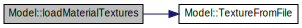
\includegraphics[width=350pt]{classModel_aa7d0215f3ee74bef71ddeef173dd36dd_cgraph}
\end{center}
\end{figure}
\mbox{\Hypertarget{classModel_a3cd88224a93dc81a8503d42be807eb86}\label{classModel_a3cd88224a93dc81a8503d42be807eb86}} 
\index{Model@{Model}!load\+Model@{load\+Model}}
\index{load\+Model@{load\+Model}!Model@{Model}}
\subsubsection{\texorpdfstring{load\+Model()}{loadModel()}}
{\footnotesize\ttfamily void Model\+::load\+Model (\begin{DoxyParamCaption}\item[{std\+::string}]{path }\end{DoxyParamCaption})\hspace{0.3cm}{\ttfamily [protected]}}



Definition at line 42 of file Model.\+cpp.



References directory\+\_\+, and process\+Node().



Referenced by Model().

Here is the call graph for this function\+:\nopagebreak
\begin{figure}[H]
\begin{center}
\leavevmode
\includegraphics[width=350pt]{classModel_a3cd88224a93dc81a8503d42be807eb86_cgraph}
\end{center}
\end{figure}
\mbox{\Hypertarget{classModel_a95ae1a9980ded3d98b1c8785cb889d96}\label{classModel_a95ae1a9980ded3d98b1c8785cb889d96}} 
\index{Model@{Model}!process\+Mesh@{process\+Mesh}}
\index{process\+Mesh@{process\+Mesh}!Model@{Model}}
\subsubsection{\texorpdfstring{process\+Mesh()}{processMesh()}}
{\footnotesize\ttfamily \mbox{\hyperlink{classMesh}{Mesh}} Model\+::process\+Mesh (\begin{DoxyParamCaption}\item[{ai\+Mesh $\ast$}]{mesh,  }\item[{const ai\+Scene $\ast$}]{scene }\end{DoxyParamCaption})\hspace{0.3cm}{\ttfamily [protected]}}



Definition at line 84 of file Model.\+cpp.



References load\+Material\+Textures(), Mesh\+::\+Vertex\+::\+Normal, Mesh\+::\+Vertex\+::\+Position, and Mesh\+::\+Vertex\+::\+Tex\+Coords.



Referenced by process\+Node().

Here is the call graph for this function\+:\nopagebreak
\begin{figure}[H]
\begin{center}
\leavevmode
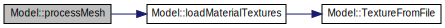
\includegraphics[width=350pt]{classModel_a95ae1a9980ded3d98b1c8785cb889d96_cgraph}
\end{center}
\end{figure}
\mbox{\Hypertarget{classModel_a23b167ce0d33f7e6ab5693cd5e81a9a5}\label{classModel_a23b167ce0d33f7e6ab5693cd5e81a9a5}} 
\index{Model@{Model}!process\+Node@{process\+Node}}
\index{process\+Node@{process\+Node}!Model@{Model}}
\subsubsection{\texorpdfstring{process\+Node()}{processNode()}}
{\footnotesize\ttfamily void Model\+::process\+Node (\begin{DoxyParamCaption}\item[{ai\+Node $\ast$}]{node,  }\item[{const ai\+Scene $\ast$}]{scene }\end{DoxyParamCaption})\hspace{0.3cm}{\ttfamily [protected]}}



Definition at line 67 of file Model.\+cpp.



References meshes\+\_\+, and process\+Mesh().



Referenced by load\+Model().

Here is the call graph for this function\+:\nopagebreak
\begin{figure}[H]
\begin{center}
\leavevmode
\includegraphics[width=350pt]{classModel_a23b167ce0d33f7e6ab5693cd5e81a9a5_cgraph}
\end{center}
\end{figure}
\mbox{\Hypertarget{classModel_a4633dd862f3066d920c2c4177a30310e}\label{classModel_a4633dd862f3066d920c2c4177a30310e}} 
\index{Model@{Model}!Texture\+From\+File@{Texture\+From\+File}}
\index{Texture\+From\+File@{Texture\+From\+File}!Model@{Model}}
\subsubsection{\texorpdfstring{Texture\+From\+File()}{TextureFromFile()}}
{\footnotesize\ttfamily G\+Lint Model\+::\+Texture\+From\+File (\begin{DoxyParamCaption}\item[{const char $\ast$}]{path,  }\item[{std\+::string}]{directory }\end{DoxyParamCaption})\hspace{0.3cm}{\ttfamily [protected]}}



Definition at line 176 of file Model.\+cpp.



Referenced by load\+Material\+Textures().



\subsection{Member Data Documentation}
\mbox{\Hypertarget{classModel_a2b8d86d272ebf7cd808a02b4d140ca12}\label{classModel_a2b8d86d272ebf7cd808a02b4d140ca12}} 
\index{Model@{Model}!directory\+\_\+@{directory\+\_\+}}
\index{directory\+\_\+@{directory\+\_\+}!Model@{Model}}
\subsubsection{\texorpdfstring{directory\+\_\+}{directory\_}}
{\footnotesize\ttfamily std\+::string Model\+::directory\+\_\+\hspace{0.3cm}{\ttfamily [private]}}



Definition at line 45 of file Model.\+h.



Referenced by load\+Material\+Textures(), and load\+Model().

\mbox{\Hypertarget{classModel_afdaef518b8ca4c7d9f95fda34f6b8ac9}\label{classModel_afdaef518b8ca4c7d9f95fda34f6b8ac9}} 
\index{Model@{Model}!meshes\+\_\+@{meshes\+\_\+}}
\index{meshes\+\_\+@{meshes\+\_\+}!Model@{Model}}
\subsubsection{\texorpdfstring{meshes\+\_\+}{meshes\_}}
{\footnotesize\ttfamily std\+::vector$<$\mbox{\hyperlink{classMesh}{Mesh}}$>$ Model\+::meshes\+\_\+\hspace{0.3cm}{\ttfamily [private]}}



Definition at line 43 of file Model.\+h.



Referenced by Draw(), and process\+Node().

\mbox{\Hypertarget{classModel_a92d229e44cb31a539ec4b5c7db977059}\label{classModel_a92d229e44cb31a539ec4b5c7db977059}} 
\index{Model@{Model}!textures\+\_\+loaded\+\_\+@{textures\+\_\+loaded\+\_\+}}
\index{textures\+\_\+loaded\+\_\+@{textures\+\_\+loaded\+\_\+}!Model@{Model}}
\subsubsection{\texorpdfstring{textures\+\_\+loaded\+\_\+}{textures\_loaded\_}}
{\footnotesize\ttfamily std\+::vector$<$\mbox{\hyperlink{structMesh_1_1Texture}{Mesh\+::\+Texture}}$>$ Model\+::textures\+\_\+loaded\+\_\+\hspace{0.3cm}{\ttfamily [private]}}



Definition at line 47 of file Model.\+h.



Referenced by has\+\_\+texture(), and load\+Material\+Textures().



The documentation for this class was generated from the following files\+:\begin{DoxyCompactItemize}
\item 
\mbox{\hyperlink{Model_8h}{Model.\+h}}\item 
\mbox{\hyperlink{Model_8cpp}{Model.\+cpp}}\end{DoxyCompactItemize}

\hypertarget{classShader}{}\section{Shader Class Reference}
\label{classShader}\index{Shader@{Shader}}


{\ttfamily \#include $<$Shader.\+h$>$}

\subsection*{Public Member Functions}
\begin{DoxyCompactItemize}
\item 
\mbox{\hyperlink{classShader_a9f793135f05ad21d6e4e4671de688d7b}{Shader}} (const std\+::string \&vertex\+\_\+shader\+\_\+path, const std\+::string \&fragment\+\_\+shader\+\_\+path)
\begin{DoxyCompactList}\small\item\em Create a shader program with given vertex and fragment shader paths. \end{DoxyCompactList}\item 
void \mbox{\hyperlink{classShader_a8e53260be208ebf6c804a0d309e74097}{install}} ()
\begin{DoxyCompactList}\small\item\em Activate the shader program. \end{DoxyCompactList}\item 
void \mbox{\hyperlink{classShader_afa6fb33b37c9385cf62a836092da570b}{uninstall}} ()
\begin{DoxyCompactList}\small\item\em Deactivate the shader program. \end{DoxyCompactList}\item 
const G\+Luint \mbox{\hyperlink{classShader_a3d9c30f7fb8c679a7389c31e51fac596}{get\+\_\+program}} ()
\end{DoxyCompactItemize}
\subsection*{Private Attributes}
\begin{DoxyCompactItemize}
\item 
G\+Luint \mbox{\hyperlink{classShader_ab1d32c11e4114a95b484f819b950af5d}{shader\+\_\+program\+\_\+id\+\_\+}}
\begin{DoxyCompactList}\small\item\em The program ID. \end{DoxyCompactList}\end{DoxyCompactItemize}


\subsection{Detailed Description}


Definition at line 17 of file Shader.\+h.



\subsection{Constructor \& Destructor Documentation}
\mbox{\Hypertarget{classShader_a9f793135f05ad21d6e4e4671de688d7b}\label{classShader_a9f793135f05ad21d6e4e4671de688d7b}} 
\index{Shader@{Shader}!Shader@{Shader}}
\index{Shader@{Shader}!Shader@{Shader}}
\subsubsection{\texorpdfstring{Shader()}{Shader()}}
{\footnotesize\ttfamily Shader\+::\+Shader (\begin{DoxyParamCaption}\item[{const std\+::string \&}]{vertex\+\_\+shader\+\_\+path,  }\item[{const std\+::string \&}]{fragment\+\_\+shader\+\_\+path }\end{DoxyParamCaption})}



Create a shader program with given vertex and fragment shader paths. 



Definition at line 18 of file Shader.\+cpp.



References shader\+\_\+program\+\_\+id\+\_\+.



\subsection{Member Function Documentation}
\mbox{\Hypertarget{classShader_a3d9c30f7fb8c679a7389c31e51fac596}\label{classShader_a3d9c30f7fb8c679a7389c31e51fac596}} 
\index{Shader@{Shader}!get\+\_\+program@{get\+\_\+program}}
\index{get\+\_\+program@{get\+\_\+program}!Shader@{Shader}}
\subsubsection{\texorpdfstring{get\+\_\+program()}{get\_program()}}
{\footnotesize\ttfamily const G\+Luint Shader\+::get\+\_\+program (\begin{DoxyParamCaption}{ }\end{DoxyParamCaption})\hspace{0.3cm}{\ttfamily [inline]}}



Definition at line 36 of file Shader.\+h.



References shader\+\_\+program\+\_\+id\+\_\+.



Referenced by Mesh\+::\+Draw(), and S\+I\+C\+A\+D\+::render\+Background().

\mbox{\Hypertarget{classShader_a8e53260be208ebf6c804a0d309e74097}\label{classShader_a8e53260be208ebf6c804a0d309e74097}} 
\index{Shader@{Shader}!install@{install}}
\index{install@{install}!Shader@{Shader}}
\subsubsection{\texorpdfstring{install()}{install()}}
{\footnotesize\ttfamily void Shader\+::install (\begin{DoxyParamCaption}{ }\end{DoxyParamCaption})}



Activate the shader program. 



Definition at line 129 of file Shader.\+cpp.



References shader\+\_\+program\+\_\+id\+\_\+.



Referenced by S\+I\+C\+A\+D\+::render\+Background().

\mbox{\Hypertarget{classShader_afa6fb33b37c9385cf62a836092da570b}\label{classShader_afa6fb33b37c9385cf62a836092da570b}} 
\index{Shader@{Shader}!uninstall@{uninstall}}
\index{uninstall@{uninstall}!Shader@{Shader}}
\subsubsection{\texorpdfstring{uninstall()}{uninstall()}}
{\footnotesize\ttfamily void Shader\+::uninstall (\begin{DoxyParamCaption}{ }\end{DoxyParamCaption})}



Deactivate the shader program. 



Definition at line 135 of file Shader.\+cpp.



Referenced by S\+I\+C\+A\+D\+::render\+Background().



\subsection{Member Data Documentation}
\mbox{\Hypertarget{classShader_ab1d32c11e4114a95b484f819b950af5d}\label{classShader_ab1d32c11e4114a95b484f819b950af5d}} 
\index{Shader@{Shader}!shader\+\_\+program\+\_\+id\+\_\+@{shader\+\_\+program\+\_\+id\+\_\+}}
\index{shader\+\_\+program\+\_\+id\+\_\+@{shader\+\_\+program\+\_\+id\+\_\+}!Shader@{Shader}}
\subsubsection{\texorpdfstring{shader\+\_\+program\+\_\+id\+\_\+}{shader\_program\_id\_}}
{\footnotesize\ttfamily G\+Luint Shader\+::shader\+\_\+program\+\_\+id\+\_\+\hspace{0.3cm}{\ttfamily [private]}}



The program ID. 



Definition at line 45 of file Shader.\+h.



Referenced by get\+\_\+program(), install(), and Shader().



The documentation for this class was generated from the following files\+:\begin{DoxyCompactItemize}
\item 
\mbox{\hyperlink{Shader_8h}{Shader.\+h}}\item 
\mbox{\hyperlink{Shader_8cpp}{Shader.\+cpp}}\end{DoxyCompactItemize}

\hypertarget{classSICAD}{}\section{S\+I\+C\+AD Class Reference}
\label{classSICAD}\index{S\+I\+C\+AD@{S\+I\+C\+AD}}


A \mbox{\hyperlink{classSuperimpose}{Superimpose}} derived class to superimpose mesh models on images.  




{\ttfamily \#include $<$S\+I\+C\+A\+D.\+h$>$}



Inheritance diagram for S\+I\+C\+AD\+:\nopagebreak
\begin{figure}[H]
\begin{center}
\leavevmode
\includegraphics[width=154pt]{classSICAD__inherit__graph}
\end{center}
\end{figure}
\subsection*{Public Types}
\begin{DoxyCompactItemize}
\item 
enum \mbox{\hyperlink{classSICAD_a7e092dede6f660355462d6d548214198}{M\+I\+P\+Maps}} \{ \mbox{\hyperlink{classSICAD_a7e092dede6f660355462d6d548214198ad879c351426770bc0b13c3628db1e636}{M\+I\+P\+Maps\+::nearest}}, 
\mbox{\hyperlink{classSICAD_a7e092dede6f660355462d6d548214198a9a932b3cb396238423eb2f33ec17d6aa}{M\+I\+P\+Maps\+::linear}}
 \}
\item 
typedef std\+::unordered\+\_\+map$<$ std\+::string, std\+::string $>$ \mbox{\hyperlink{classSICAD_a9e1e1460d4c0f331b4fd015aae4dd721}{Model\+Path\+Container}}
\item 
typedef std\+::pair$<$ std\+::string, std\+::string $>$ \mbox{\hyperlink{classSICAD_a5148c8a96c82625706ce2e5b86b52dd7}{Model\+Path\+Element}}
\item 
typedef std\+::unordered\+\_\+map$<$ std\+::string, \mbox{\hyperlink{classModel}{Model}} $\ast$ $>$ \mbox{\hyperlink{classSICAD_aca3c9693d298f2e8dc171194c6a7507c}{Model\+Container}}
\item 
typedef std\+::pair$<$ std\+::string, \mbox{\hyperlink{classModel}{Model}} $\ast$ $>$ \mbox{\hyperlink{classSICAD_af999665097d7cdf11780735bf24a6956}{Model\+Element}}
\item 
typedef std\+::vector$<$ double $>$ \mbox{\hyperlink{classSuperimpose_a85d40a5caf19f486d1e0c15c0a025378}{Model\+Pose}}
\item 
typedef std\+::multimap$<$ std\+::string, \mbox{\hyperlink{classSuperimpose_a85d40a5caf19f486d1e0c15c0a025378}{Model\+Pose}} $>$ \mbox{\hyperlink{classSuperimpose_a178e3d4e2def6635bfcf9454dd4b5d22}{Model\+Pose\+Container}}
\item 
typedef std\+::pair$<$ std\+::string, \mbox{\hyperlink{classSuperimpose_a85d40a5caf19f486d1e0c15c0a025378}{Model\+Pose}} $>$ \mbox{\hyperlink{classSuperimpose_a1e02e0225687b42296dcfee4eadf8a55}{Model\+Pose\+Container\+Element}}
\end{DoxyCompactItemize}
\subsection*{Public Member Functions}
\begin{DoxyCompactItemize}
\item 
\mbox{\hyperlink{classSICAD_a4ff326a5104dad4c81898d3dd344205d}{S\+I\+C\+AD}} (const \mbox{\hyperlink{classSICAD_a9e1e1460d4c0f331b4fd015aae4dd721}{Model\+Path\+Container}} \&objfile\+\_\+map, const G\+Lsizei cam\+\_\+width, const G\+Lsizei cam\+\_\+height, const G\+Lfloat cam\+\_\+fx, const G\+Lfloat cam\+\_\+fy, const G\+Lfloat cam\+\_\+cx, const G\+Lfloat cam\+\_\+cy)
\begin{DoxyCompactList}\small\item\em Create a \mbox{\hyperlink{classSICAD}{S\+I\+C\+AD}} object with a dedicated Open\+GL context and default shaders. \end{DoxyCompactList}\item 
\mbox{\hyperlink{classSICAD_aa164d674fd047a3522efe18450094ab7}{S\+I\+C\+AD}} (const \mbox{\hyperlink{classSICAD_a9e1e1460d4c0f331b4fd015aae4dd721}{Model\+Path\+Container}} \&objfile\+\_\+map, const G\+Lsizei cam\+\_\+width, const G\+Lsizei cam\+\_\+height, const G\+Lfloat cam\+\_\+fx, const G\+Lfloat cam\+\_\+fy, const G\+Lfloat cam\+\_\+cx, const G\+Lfloat cam\+\_\+cy, const G\+Lint num\+\_\+images)
\begin{DoxyCompactList}\small\item\em Create a \mbox{\hyperlink{classSICAD}{S\+I\+C\+AD}} object with a dedicated Open\+GL context and default shaders. \end{DoxyCompactList}\item 
\mbox{\hyperlink{classSICAD_a3224c268f057e1eb18f6cf42ad099402}{S\+I\+C\+AD}} (const \mbox{\hyperlink{classSICAD_a9e1e1460d4c0f331b4fd015aae4dd721}{Model\+Path\+Container}} \&objfile\+\_\+map, const G\+Lsizei cam\+\_\+width, const G\+Lsizei cam\+\_\+height, const G\+Lfloat cam\+\_\+fx, const G\+Lfloat cam\+\_\+fy, const G\+Lfloat cam\+\_\+cx, const G\+Lfloat cam\+\_\+cy, const G\+Lint num\+\_\+images, const std\+::string \&shader\+\_\+folder)
\begin{DoxyCompactList}\small\item\em Create a \mbox{\hyperlink{classSICAD}{S\+I\+C\+AD}} object with a dedicated Open\+GL context and custom shaders. \end{DoxyCompactList}\item 
\mbox{\hyperlink{classSICAD_a2d0feeca1d62a456f861046e377cd303}{S\+I\+C\+AD}} (const \mbox{\hyperlink{classSICAD_a9e1e1460d4c0f331b4fd015aae4dd721}{Model\+Path\+Container}} \&objfile\+\_\+map, const G\+Lsizei cam\+\_\+width, const G\+Lsizei cam\+\_\+height, const G\+Lfloat cam\+\_\+fx, const G\+Lfloat cam\+\_\+fy, const G\+Lfloat cam\+\_\+cx, const G\+Lfloat cam\+\_\+cy, const G\+Lint num\+\_\+images, const std\+::string \&shader\+\_\+folder, const std\+::vector$<$ float $>$ \&ogl\+\_\+to\+\_\+cam)
\begin{DoxyCompactList}\small\item\em Create a \mbox{\hyperlink{classSICAD}{S\+I\+C\+AD}} object with a dedicated Open\+GL context and custom shaders. \end{DoxyCompactList}\item 
virtual \mbox{\hyperlink{classSICAD_a4e3d6d1f90ea2261dcd8507ee8709360}{$\sim$\+S\+I\+C\+AD}} ()
\item 
bool \mbox{\hyperlink{classSICAD_aaf003ab2ac8bc5ebdef6611ca1547e73}{get\+Ogl\+Window\+Should\+Close}} ()
\item 
void \mbox{\hyperlink{classSICAD_a0e42acab32252ddc878794f365ee1037}{set\+Ogl\+Window\+Should\+Close}} (bool should\+\_\+close)
\item 
bool \mbox{\hyperlink{classSICAD_a356e0ac8a0f130952a72326bedd4ab60}{superimpose}} (const \mbox{\hyperlink{classSuperimpose_a178e3d4e2def6635bfcf9454dd4b5d22}{Model\+Pose\+Container}} \&objpos\+\_\+map, const double $\ast$cam\+\_\+x, const double $\ast$cam\+\_\+o, cv\+::\+Mat \&img) override
\begin{DoxyCompactList}\small\item\em Render the mesh models in the pose specified in {\ttfamily objpos\+\_\+map} and move the virtual camera in {\ttfamily cam\+\_\+x} position with orientation {\ttfamily cam\+\_\+o}. \end{DoxyCompactList}\item 
virtual bool \mbox{\hyperlink{classSICAD_ab15f84cec5a65c8dd6cad85f9b0e1993}{superimpose}} (const std\+::vector$<$ \mbox{\hyperlink{classSuperimpose_a178e3d4e2def6635bfcf9454dd4b5d22}{Model\+Pose\+Container}} $>$ \&objpos\+\_\+multimap, const double $\ast$cam\+\_\+x, const double $\ast$cam\+\_\+o, cv\+::\+Mat \&img)
\begin{DoxyCompactList}\small\item\em Render the mesh models in the pose specified in each element of {\ttfamily objpos\+\_\+multimap} and move the virtual camera in {\ttfamily cam\+\_\+x} position with orientation {\ttfamily cam\+\_\+o}. \end{DoxyCompactList}\item 
virtual bool \mbox{\hyperlink{classSICAD_af6c19a679de29992c5f9609f4424add0}{superimpose}} (const \mbox{\hyperlink{classSuperimpose_a178e3d4e2def6635bfcf9454dd4b5d22}{Model\+Pose\+Container}} \&objpos\+\_\+map, const double $\ast$cam\+\_\+x, const double $\ast$cam\+\_\+o, cv\+::\+Mat \&img, const G\+Lsizei cam\+\_\+width, const G\+Lsizei cam\+\_\+height, const G\+Lfloat cam\+\_\+fx, const G\+Lfloat cam\+\_\+fy, const G\+Lfloat cam\+\_\+cx, const G\+Lfloat cam\+\_\+cy)
\item 
virtual bool \mbox{\hyperlink{classSICAD_a269e238387393b44177daa4eae88fedd}{superimpose}} (const std\+::vector$<$ \mbox{\hyperlink{classSuperimpose_a178e3d4e2def6635bfcf9454dd4b5d22}{Model\+Pose\+Container}} $>$ \&objpos\+\_\+multimap, const double $\ast$cam\+\_\+x, const double $\ast$cam\+\_\+o, cv\+::\+Mat \&img, const G\+Lsizei cam\+\_\+width, const G\+Lsizei cam\+\_\+height, const G\+Lfloat cam\+\_\+fx, const G\+Lfloat cam\+\_\+fy, const G\+Lfloat cam\+\_\+cx, const G\+Lfloat cam\+\_\+cy)
\item 
virtual bool \mbox{\hyperlink{classSICAD_a5a76058edfdeed2b37b40bde2eec3db1}{superimpose}} (const \mbox{\hyperlink{classSuperimpose_a178e3d4e2def6635bfcf9454dd4b5d22}{Model\+Pose\+Container}} \&objpos\+\_\+map, const double $\ast$cam\+\_\+x, const double $\ast$cam\+\_\+o, const size\+\_\+t pbo\+\_\+index)
\begin{DoxyCompactList}\small\item\em Render the mesh models in the pose specified in {\ttfamily objpos\+\_\+map} and move the virtual camera in {\ttfamily cam\+\_\+x} position with orientation {\ttfamily cam\+\_\+o}. \end{DoxyCompactList}\item 
virtual bool \mbox{\hyperlink{classSICAD_a0dfbfdd508faf5f07a58ddfb6b9da50b}{superimpose}} (const \mbox{\hyperlink{classSuperimpose_a178e3d4e2def6635bfcf9454dd4b5d22}{Model\+Pose\+Container}} \&objpos\+\_\+map, const double $\ast$cam\+\_\+x, const double $\ast$cam\+\_\+o, const size\+\_\+t pbo\+\_\+index, const cv\+::\+Mat \&img)
\begin{DoxyCompactList}\small\item\em Render the mesh models in the pose specified in {\ttfamily objpos\+\_\+map} and move the virtual camera in {\ttfamily cam\+\_\+x} position with orientation {\ttfamily cam\+\_\+o}. \end{DoxyCompactList}\item 
virtual bool \mbox{\hyperlink{classSICAD_acf0ea95ecb121c0b265ca52ac589d80f}{superimpose}} (const std\+::vector$<$ \mbox{\hyperlink{classSuperimpose_a178e3d4e2def6635bfcf9454dd4b5d22}{Model\+Pose\+Container}} $>$ \&objpos\+\_\+multimap, const double $\ast$cam\+\_\+x, const double $\ast$cam\+\_\+o, const size\+\_\+t pbo\+\_\+index)
\begin{DoxyCompactList}\small\item\em Render the mesh models in the pose specified in each element of {\ttfamily objpos\+\_\+multimap} and move the virtual camera in {\ttfamily cam\+\_\+x} position with orientation {\ttfamily cam\+\_\+o}. \end{DoxyCompactList}\item 
virtual bool \mbox{\hyperlink{classSICAD_a264db68e6189b5907d162947267be056}{superimpose}} (const std\+::vector$<$ \mbox{\hyperlink{classSuperimpose_a178e3d4e2def6635bfcf9454dd4b5d22}{Model\+Pose\+Container}} $>$ \&objpos\+\_\+multimap, const double $\ast$cam\+\_\+x, const double $\ast$cam\+\_\+o, const size\+\_\+t pbo\+\_\+index, const cv\+::\+Mat \&img)
\begin{DoxyCompactList}\small\item\em Render the mesh models in the pose specified in each element of {\ttfamily objpos\+\_\+multimap} and move the virtual camera in {\ttfamily cam\+\_\+x} position with orientation {\ttfamily cam\+\_\+o}. \end{DoxyCompactList}\item 
virtual void \mbox{\hyperlink{classSICAD_ae626fa7f8fd4dc5fc4bdc4f5311beede}{release\+Context}} () const
\begin{DoxyCompactList}\small\item\em Make the current thread Open\+GL context not current. \end{DoxyCompactList}\item 
std\+::pair$<$ const G\+Luint $\ast$, size\+\_\+t $>$ \mbox{\hyperlink{classSICAD_a02c1c9f6c83bd9df278cdcfdaa78ccf4}{get\+P\+B\+Os}} () const
\begin{DoxyCompactList}\small\item\em Returns the Pixel Buffer Object (P\+BO) vector and its size. \end{DoxyCompactList}\item 
std\+::pair$<$ bool, G\+Luint $>$ \mbox{\hyperlink{classSICAD_adb0158ae3b9e5741df2fae4d50280809}{get\+P\+BO}} (const size\+\_\+t pbo\+\_\+index) const
\begin{DoxyCompactList}\small\item\em Returns {\ttfamily pbo\+\_\+index}-\/th Pixel Buffer Object (P\+BO) value. \end{DoxyCompactList}\item 
bool \mbox{\hyperlink{classSICAD_a39cdff6871d32429d8ba95b776e0b874}{set\+Projection\+Matrix}} (const G\+Lsizei cam\+\_\+width, const G\+Lsizei cam\+\_\+height, const G\+Lfloat cam\+\_\+fx, const G\+Lfloat cam\+\_\+fy, const G\+Lfloat cam\+\_\+cx, const G\+Lfloat cam\+\_\+cy)
\item 
bool \mbox{\hyperlink{classSICAD_a170bd325654aed9eb81062ac610608fa}{get\+Background\+Opt}} () const
\item 
void \mbox{\hyperlink{classSICAD_a07921943ad3d4016dcbe76135e799754}{set\+Background\+Opt}} (bool show\+\_\+background)
\item 
G\+Lenum \mbox{\hyperlink{classSICAD_af65b5ad73e2c0e872face157b56bd68b}{get\+Wireframe\+Opt}} () const
\item 
void \mbox{\hyperlink{classSICAD_a4cf80a273b6b0d946cd298472c63ddd4}{set\+Wireframe\+Opt}} (bool show\+\_\+mesh\+\_\+wires)
\item 
void \mbox{\hyperlink{classSICAD_a1fa052a3609f52156b472e872e34971a}{set\+Mipmaps\+Opt}} (const \mbox{\hyperlink{classSICAD_a7e092dede6f660355462d6d548214198}{M\+I\+P\+Maps}} \&mipmaps)
\item 
\mbox{\hyperlink{classSICAD_a7e092dede6f660355462d6d548214198}{M\+I\+P\+Maps}} \mbox{\hyperlink{classSICAD_a8033a99745f595ea5205e3830cabc389}{get\+Mipmaps\+Opt}} () const
\item 
int \mbox{\hyperlink{classSICAD_a728f82ebbfeea54f3fef2fc0c56a4964}{get\+Tiles\+Number}} () const
\item 
int \mbox{\hyperlink{classSICAD_a9e3dd48dfd83ea0bd00d64dacc4fbd40}{get\+Tiles\+Rows}} () const
\item 
int \mbox{\hyperlink{classSICAD_a2ba3a0aeb3dab9996bdeed19a16eae56}{get\+Tiles\+Cols}} () const
\end{DoxyCompactItemize}
\subsection*{Private Member Functions}
\begin{DoxyCompactItemize}
\item 
glm\+::mat4 \mbox{\hyperlink{classSICAD_a1bdece095865249df4cb4e6a7ad2901e}{get\+View\+Transformation\+Matrix}} (const double $\ast$cam\+\_\+x, const double $\ast$cam\+\_\+o)
\item 
void \mbox{\hyperlink{classSICAD_a8238a2b2c488c8b7ba85d5b2a0bf00ac}{poll\+Or\+Post\+Event}} ()
\item 
void \mbox{\hyperlink{classSICAD_a46fcf7ddb480a788463a4d98d26e12e8}{render\+Background}} (const cv\+::\+Mat \&img) const
\item 
void \mbox{\hyperlink{classSICAD_ae7af7aba5d81b9f1cc3e273a55811a70}{set\+Wireframe}} (G\+Lenum mode)
\item 
void \mbox{\hyperlink{classSICAD_a2603ec5cb9a31bc7be0a335ef513ab0d}{factorize\+\_\+int}} (const G\+Lsizei area, const G\+Lsizei width\+\_\+limit, const G\+Lsizei height\+\_\+limit, G\+Lsizei \&width, G\+Lsizei \&height)
\end{DoxyCompactItemize}
\subsection*{Private Attributes}
\begin{DoxyCompactItemize}
\item 
const std\+::string \mbox{\hyperlink{classSICAD_a9eb34b659cac13b8442ca821455cc1f1}{log\+\_\+\+I\+D\+\_\+}} = \char`\"{}\mbox{[}S\+I\+::\+S\+I\+C\+AD\mbox{]}\char`\"{}
\item 
G\+L\+F\+Wwindow $\ast$ \mbox{\hyperlink{classSICAD_a3e55fa9ffa99ef200bfc15d6a105698a}{window\+\_\+}} = nullptr
\item 
G\+Lint \mbox{\hyperlink{classSICAD_a68723ee57cc9a1e02bc0dbda54a584ff}{tiles\+\_\+num\+\_\+}} = 0
\item 
G\+Lsizei \mbox{\hyperlink{classSICAD_ac2678cc1ad1b008912fec7e6892b23e1}{tiles\+\_\+cols\+\_\+}} = 0
\item 
G\+Lsizei \mbox{\hyperlink{classSICAD_aca3efa8f3fb75b3ee02474d4ec00e49e}{tiles\+\_\+rows\+\_\+}} = 0
\item 
G\+Lsizei \mbox{\hyperlink{classSICAD_ade37d5c3960d164acaa749745f55070f}{image\+\_\+width\+\_\+}} = 0
\item 
G\+Lsizei \mbox{\hyperlink{classSICAD_a093da94bc84a46d08f71051c4d88c176}{image\+\_\+height\+\_\+}} = 0
\item 
glm\+::mat3 \mbox{\hyperlink{classSICAD_a95af2758122e6420369516fd13fd03cc}{ogl\+\_\+to\+\_\+cam\+\_\+}} = glm\+::mat3(1.\+0f)
\item 
G\+Lsizei \mbox{\hyperlink{classSICAD_a08c86b826a1784b132bac3f0792fc604}{framebuffer\+\_\+width\+\_\+}} = 0
\item 
G\+Lsizei \mbox{\hyperlink{classSICAD_a3361bb03e52bc0554bb1e3670ef3a0f9}{framebuffer\+\_\+height\+\_\+}} = 0
\item 
G\+Lsizei \mbox{\hyperlink{classSICAD_a1dda156a616e004de5364914d8d6c4b9}{tile\+\_\+img\+\_\+width\+\_\+}} = 0
\item 
G\+Lsizei \mbox{\hyperlink{classSICAD_a2e6b01258527769e4066262ed002fc69}{tile\+\_\+img\+\_\+height\+\_\+}} = 0
\item 
const G\+Lfloat \mbox{\hyperlink{classSICAD_a690437655965101bad97d32e98015dd5}{near\+\_\+}} = 0.\+001f
\item 
const G\+Lfloat \mbox{\hyperlink{classSICAD_a4c4d2e249ac824528e1fe9f97fa207d9}{far\+\_\+}} = 1000.\+0f
\item 
std\+::thread\+::id \mbox{\hyperlink{classSICAD_a6a4623d27b2ee48ad0db90bd075c708c}{main\+\_\+thread\+\_\+id\+\_\+}}
\item 
bool \mbox{\hyperlink{classSICAD_a8db9e37d71a14883be4879e9ea4b6a02}{show\+\_\+background\+\_\+}} = false
\item 
G\+Lenum \mbox{\hyperlink{classSICAD_a9c4c3ba5d071f763ee1956fa31faa3f8}{show\+\_\+mesh\+\_\+mode\+\_\+}} = G\+L\+\_\+\+F\+I\+LL
\item 
\mbox{\hyperlink{classSICAD_a7e092dede6f660355462d6d548214198}{M\+I\+P\+Maps}} \mbox{\hyperlink{classSICAD_a34b0de96321855145937cc5858c019b0}{mesh\+\_\+mmaps\+\_\+}} = \mbox{\hyperlink{classSICAD_a7e092dede6f660355462d6d548214198ad879c351426770bc0b13c3628db1e636}{M\+I\+P\+Maps\+::nearest}}
\item 
\mbox{\hyperlink{classShader}{Shader}} $\ast$ \mbox{\hyperlink{classSICAD_a46edf33acc9f7ea3bd98c7ee6388ce9c}{shader\+\_\+background\+\_\+}} = nullptr
\item 
\mbox{\hyperlink{classShader}{Shader}} $\ast$ \mbox{\hyperlink{classSICAD_a6c11f0e8dc8cbdd91748c230fc680833}{shader\+\_\+cad\+\_\+}} = nullptr
\item 
std\+::unique\+\_\+ptr$<$ \mbox{\hyperlink{classShader}{Shader}} $>$ \mbox{\hyperlink{classSICAD_aa9c575d7847080ed891015f457a8fd59}{shader\+\_\+mesh\+\_\+texture\+\_\+}}
\item 
\mbox{\hyperlink{classShader}{Shader}} $\ast$ \mbox{\hyperlink{classSICAD_ac921e60623f3797253bcbcdd445b903b}{shader\+\_\+frame\+\_\+}} = nullptr
\item 
\mbox{\hyperlink{classSICAD_aca3c9693d298f2e8dc171194c6a7507c}{Model\+Container}} \mbox{\hyperlink{classSICAD_a05fea2b5b027a3b7f37ef9ea4ecd64f0}{model\+\_\+obj\+\_\+}}
\item 
G\+Luint \mbox{\hyperlink{classSICAD_a2c173ad18d42e090b46a539f92f3fe9d}{fbo\+\_\+}}
\item 
G\+Luint \mbox{\hyperlink{classSICAD_a50f1ec3b2545ca40d58466735da80fc6}{texture\+\_\+color\+\_\+buffer\+\_\+}}
\item 
G\+Luint \mbox{\hyperlink{classSICAD_a2fed5ac56bb2206fe8f6eccc9d784015}{texture\+\_\+depth\+\_\+buffer\+\_\+}}
\item 
G\+Luint \mbox{\hyperlink{classSICAD_a2728fb0fa0be11f0992bc81b4873da4f}{texture\+\_\+background\+\_\+}}
\item 
G\+Luint \mbox{\hyperlink{classSICAD_a19306fe768bae547e18a3b9366e37389}{vao\+\_\+background\+\_\+}}
\item 
G\+Luint \mbox{\hyperlink{classSICAD_a2cdcd11dd55a4b02b85d7c32435cc719}{ebo\+\_\+background\+\_\+}}
\item 
G\+Luint \mbox{\hyperlink{classSICAD_a86d6184b8c557460317a158e8d9508d1}{vbo\+\_\+background\+\_\+}}
\item 
G\+Luint \mbox{\hyperlink{classSICAD_ae91abeb0fe30f27e0fc40649235f3437}{vao\+\_\+frame\+\_\+}}
\item 
G\+Luint \mbox{\hyperlink{classSICAD_af58ffe3edf622ab96f669fcd6e210be9}{vbo\+\_\+frame\+\_\+}}
\item 
size\+\_\+t \mbox{\hyperlink{classSICAD_a3d7e1e1b3049508ea3c40b85541ea818}{pbo\+\_\+number\+\_\+}} = 2
\item 
G\+Luint \mbox{\hyperlink{classSICAD_a56b765675245d3b4501cfda799d4630a}{pbo\+\_\+}} \mbox{[}2\mbox{]}
\item 
glm\+::mat4 \mbox{\hyperlink{classSICAD_ad5945f84df0d90113a24b2001ecbc832}{back\+\_\+proj\+\_\+}}
\item 
glm\+::mat4 \mbox{\hyperlink{classSICAD_afb91b682fd1f6629f163ab321869e7e0}{projection\+\_\+}}
\end{DoxyCompactItemize}
\subsection*{Static Private Attributes}
\begin{DoxyCompactItemize}
\item 
static int \mbox{\hyperlink{classSICAD_a16f7c3c77ddea5ba57bbcbcdd7a8d125}{class\+\_\+counter\+\_\+}} = 0
\item 
static G\+Lsizei \mbox{\hyperlink{classSICAD_aca24504d58ce97106dbc95925f36fca0}{renderbuffer\+\_\+size\+\_\+}} = 0
\end{DoxyCompactItemize}


\subsection{Detailed Description}
A \mbox{\hyperlink{classSuperimpose}{Superimpose}} derived class to superimpose mesh models on images. 

Definition at line 30 of file S\+I\+C\+A\+D.\+h.



\subsection{Member Typedef Documentation}
\mbox{\Hypertarget{classSICAD_aca3c9693d298f2e8dc171194c6a7507c}\label{classSICAD_aca3c9693d298f2e8dc171194c6a7507c}} 
\index{S\+I\+C\+AD@{S\+I\+C\+AD}!Model\+Container@{Model\+Container}}
\index{Model\+Container@{Model\+Container}!S\+I\+C\+AD@{S\+I\+C\+AD}}
\subsubsection{\texorpdfstring{Model\+Container}{ModelContainer}}
{\footnotesize\ttfamily typedef std\+::unordered\+\_\+map$<$std\+::string, \mbox{\hyperlink{classModel}{Model}}$\ast$$>$ \mbox{\hyperlink{classSICAD_aca3c9693d298f2e8dc171194c6a7507c}{S\+I\+C\+A\+D\+::\+Model\+Container}}}



Definition at line 37 of file S\+I\+C\+A\+D.\+h.

\mbox{\Hypertarget{classSICAD_af999665097d7cdf11780735bf24a6956}\label{classSICAD_af999665097d7cdf11780735bf24a6956}} 
\index{S\+I\+C\+AD@{S\+I\+C\+AD}!Model\+Element@{Model\+Element}}
\index{Model\+Element@{Model\+Element}!S\+I\+C\+AD@{S\+I\+C\+AD}}
\subsubsection{\texorpdfstring{Model\+Element}{ModelElement}}
{\footnotesize\ttfamily typedef std\+::pair$<$std\+::string, \mbox{\hyperlink{classModel}{Model}}$\ast$$>$ \mbox{\hyperlink{classSICAD_af999665097d7cdf11780735bf24a6956}{S\+I\+C\+A\+D\+::\+Model\+Element}}}



Definition at line 39 of file S\+I\+C\+A\+D.\+h.

\mbox{\Hypertarget{classSICAD_a9e1e1460d4c0f331b4fd015aae4dd721}\label{classSICAD_a9e1e1460d4c0f331b4fd015aae4dd721}} 
\index{S\+I\+C\+AD@{S\+I\+C\+AD}!Model\+Path\+Container@{Model\+Path\+Container}}
\index{Model\+Path\+Container@{Model\+Path\+Container}!S\+I\+C\+AD@{S\+I\+C\+AD}}
\subsubsection{\texorpdfstring{Model\+Path\+Container}{ModelPathContainer}}
{\footnotesize\ttfamily typedef std\+::unordered\+\_\+map$<$std\+::string, std\+::string$>$ \mbox{\hyperlink{classSICAD_a9e1e1460d4c0f331b4fd015aae4dd721}{S\+I\+C\+A\+D\+::\+Model\+Path\+Container}}}



Definition at line 33 of file S\+I\+C\+A\+D.\+h.

\mbox{\Hypertarget{classSICAD_a5148c8a96c82625706ce2e5b86b52dd7}\label{classSICAD_a5148c8a96c82625706ce2e5b86b52dd7}} 
\index{S\+I\+C\+AD@{S\+I\+C\+AD}!Model\+Path\+Element@{Model\+Path\+Element}}
\index{Model\+Path\+Element@{Model\+Path\+Element}!S\+I\+C\+AD@{S\+I\+C\+AD}}
\subsubsection{\texorpdfstring{Model\+Path\+Element}{ModelPathElement}}
{\footnotesize\ttfamily typedef std\+::pair$<$std\+::string, std\+::string$>$ \mbox{\hyperlink{classSICAD_a5148c8a96c82625706ce2e5b86b52dd7}{S\+I\+C\+A\+D\+::\+Model\+Path\+Element}}}



Definition at line 35 of file S\+I\+C\+A\+D.\+h.

\mbox{\Hypertarget{classSuperimpose_a85d40a5caf19f486d1e0c15c0a025378}\label{classSuperimpose_a85d40a5caf19f486d1e0c15c0a025378}} 
\index{S\+I\+C\+AD@{S\+I\+C\+AD}!Model\+Pose@{Model\+Pose}}
\index{Model\+Pose@{Model\+Pose}!S\+I\+C\+AD@{S\+I\+C\+AD}}
\subsubsection{\texorpdfstring{Model\+Pose}{ModelPose}}
{\footnotesize\ttfamily typedef std\+::vector$<$double$>$ \mbox{\hyperlink{classSuperimpose_a85d40a5caf19f486d1e0c15c0a025378}{Superimpose\+::\+Model\+Pose}}\hspace{0.3cm}{\ttfamily [inherited]}}



Definition at line 23 of file Superimpose.\+h.

\mbox{\Hypertarget{classSuperimpose_a178e3d4e2def6635bfcf9454dd4b5d22}\label{classSuperimpose_a178e3d4e2def6635bfcf9454dd4b5d22}} 
\index{S\+I\+C\+AD@{S\+I\+C\+AD}!Model\+Pose\+Container@{Model\+Pose\+Container}}
\index{Model\+Pose\+Container@{Model\+Pose\+Container}!S\+I\+C\+AD@{S\+I\+C\+AD}}
\subsubsection{\texorpdfstring{Model\+Pose\+Container}{ModelPoseContainer}}
{\footnotesize\ttfamily typedef std\+::multimap$<$std\+::string, \mbox{\hyperlink{classSuperimpose_a85d40a5caf19f486d1e0c15c0a025378}{Model\+Pose}}$>$ \mbox{\hyperlink{classSuperimpose_a178e3d4e2def6635bfcf9454dd4b5d22}{Superimpose\+::\+Model\+Pose\+Container}}\hspace{0.3cm}{\ttfamily [inherited]}}



Definition at line 25 of file Superimpose.\+h.

\mbox{\Hypertarget{classSuperimpose_a1e02e0225687b42296dcfee4eadf8a55}\label{classSuperimpose_a1e02e0225687b42296dcfee4eadf8a55}} 
\index{S\+I\+C\+AD@{S\+I\+C\+AD}!Model\+Pose\+Container\+Element@{Model\+Pose\+Container\+Element}}
\index{Model\+Pose\+Container\+Element@{Model\+Pose\+Container\+Element}!S\+I\+C\+AD@{S\+I\+C\+AD}}
\subsubsection{\texorpdfstring{Model\+Pose\+Container\+Element}{ModelPoseContainerElement}}
{\footnotesize\ttfamily typedef std\+::pair$<$std\+::string, \mbox{\hyperlink{classSuperimpose_a85d40a5caf19f486d1e0c15c0a025378}{Model\+Pose}}$>$ \mbox{\hyperlink{classSuperimpose_a1e02e0225687b42296dcfee4eadf8a55}{Superimpose\+::\+Model\+Pose\+Container\+Element}}\hspace{0.3cm}{\ttfamily [inherited]}}



Definition at line 27 of file Superimpose.\+h.



\subsection{Member Enumeration Documentation}
\mbox{\Hypertarget{classSICAD_a7e092dede6f660355462d6d548214198}\label{classSICAD_a7e092dede6f660355462d6d548214198}} 
\index{S\+I\+C\+AD@{S\+I\+C\+AD}!M\+I\+P\+Maps@{M\+I\+P\+Maps}}
\index{M\+I\+P\+Maps@{M\+I\+P\+Maps}!S\+I\+C\+AD@{S\+I\+C\+AD}}
\subsubsection{\texorpdfstring{M\+I\+P\+Maps}{MIPMaps}}
{\footnotesize\ttfamily enum \mbox{\hyperlink{classSICAD_a7e092dede6f660355462d6d548214198}{S\+I\+C\+A\+D\+::\+M\+I\+P\+Maps}}\hspace{0.3cm}{\ttfamily [strong]}}

\begin{DoxyEnumFields}{Enumerator}
\raisebox{\heightof{T}}[0pt][0pt]{\index{nearest@{nearest}!S\+I\+C\+AD@{S\+I\+C\+AD}}\index{S\+I\+C\+AD@{S\+I\+C\+AD}!nearest@{nearest}}}\mbox{\Hypertarget{classSICAD_a7e092dede6f660355462d6d548214198ad879c351426770bc0b13c3628db1e636}\label{classSICAD_a7e092dede6f660355462d6d548214198ad879c351426770bc0b13c3628db1e636}} 
nearest&\\
\hline

\raisebox{\heightof{T}}[0pt][0pt]{\index{linear@{linear}!S\+I\+C\+AD@{S\+I\+C\+AD}}\index{S\+I\+C\+AD@{S\+I\+C\+AD}!linear@{linear}}}\mbox{\Hypertarget{classSICAD_a7e092dede6f660355462d6d548214198a9a932b3cb396238423eb2f33ec17d6aa}\label{classSICAD_a7e092dede6f660355462d6d548214198a9a932b3cb396238423eb2f33ec17d6aa}} 
linear&\\
\hline

\end{DoxyEnumFields}


Definition at line 41 of file S\+I\+C\+A\+D.\+h.



\subsection{Constructor \& Destructor Documentation}
\mbox{\Hypertarget{classSICAD_a4ff326a5104dad4c81898d3dd344205d}\label{classSICAD_a4ff326a5104dad4c81898d3dd344205d}} 
\index{S\+I\+C\+AD@{S\+I\+C\+AD}!S\+I\+C\+AD@{S\+I\+C\+AD}}
\index{S\+I\+C\+AD@{S\+I\+C\+AD}!S\+I\+C\+AD@{S\+I\+C\+AD}}
\subsubsection{\texorpdfstring{S\+I\+C\+A\+D()}{SICAD()}\hspace{0.1cm}{\footnotesize\ttfamily [1/4]}}
{\footnotesize\ttfamily S\+I\+C\+A\+D\+::\+S\+I\+C\+AD (\begin{DoxyParamCaption}\item[{const \mbox{\hyperlink{classSICAD_a9e1e1460d4c0f331b4fd015aae4dd721}{Model\+Path\+Container}} \&}]{objfile\+\_\+map,  }\item[{const G\+Lsizei}]{cam\+\_\+width,  }\item[{const G\+Lsizei}]{cam\+\_\+height,  }\item[{const G\+Lfloat}]{cam\+\_\+fx,  }\item[{const G\+Lfloat}]{cam\+\_\+fy,  }\item[{const G\+Lfloat}]{cam\+\_\+cx,  }\item[{const G\+Lfloat}]{cam\+\_\+cy }\end{DoxyParamCaption})}



Create a \mbox{\hyperlink{classSICAD}{S\+I\+C\+AD}} object with a dedicated Open\+GL context and default shaders. 

Only 1 image will be rendered in the Open\+GL context.

The reference frame of the Open\+GL virtual camera is the standard right-\/handed system and can be changed by means of {\ttfamily ogl\+\_\+to\+\_\+cam} parameter.


\begin{DoxyParams}{Parameters}
{\em objfile\+\_\+map} & A (tag, path) container to associate a \textquotesingle{}tag\textquotesingle{} to the mesh file specified in \textquotesingle{}path\textquotesingle{}. \\
\hline
{\em cam\+\_\+width} & Camera or image width. \\
\hline
{\em cam\+\_\+height} & Camera or image height. \\
\hline
{\em cam\+\_\+fx} & focal Length along the x axis in pixels. \\
\hline
{\em cam\+\_\+fy} & focal Length along the y axis in pixels. \\
\hline
\end{DoxyParams}


Definition at line 29 of file S\+I\+C\+A\+D.\+cpp.

\mbox{\Hypertarget{classSICAD_aa164d674fd047a3522efe18450094ab7}\label{classSICAD_aa164d674fd047a3522efe18450094ab7}} 
\index{S\+I\+C\+AD@{S\+I\+C\+AD}!S\+I\+C\+AD@{S\+I\+C\+AD}}
\index{S\+I\+C\+AD@{S\+I\+C\+AD}!S\+I\+C\+AD@{S\+I\+C\+AD}}
\subsubsection{\texorpdfstring{S\+I\+C\+A\+D()}{SICAD()}\hspace{0.1cm}{\footnotesize\ttfamily [2/4]}}
{\footnotesize\ttfamily S\+I\+C\+A\+D\+::\+S\+I\+C\+AD (\begin{DoxyParamCaption}\item[{const \mbox{\hyperlink{classSICAD_a9e1e1460d4c0f331b4fd015aae4dd721}{Model\+Path\+Container}} \&}]{objfile\+\_\+map,  }\item[{const G\+Lsizei}]{cam\+\_\+width,  }\item[{const G\+Lsizei}]{cam\+\_\+height,  }\item[{const G\+Lfloat}]{cam\+\_\+fx,  }\item[{const G\+Lfloat}]{cam\+\_\+fy,  }\item[{const G\+Lfloat}]{cam\+\_\+cx,  }\item[{const G\+Lfloat}]{cam\+\_\+cy,  }\item[{const G\+Lint}]{num\+\_\+images }\end{DoxyParamCaption})}



Create a \mbox{\hyperlink{classSICAD}{S\+I\+C\+AD}} object with a dedicated Open\+GL context and default shaders. 

Up to {\ttfamily num\+\_\+images} images will be rendered in the same Open\+GL context and the result of the process will be tiled up in a regular grid. This implies that the total number of rendered images may be less than or equal to the required {\ttfamily num\+\_\+images}. The total number of rendered images is chosen to optimize performance and accessibility and can be accessed through {\ttfamily \mbox{\hyperlink{classSICAD_a728f82ebbfeea54f3fef2fc0c56a4964}{S\+I\+C\+A\+D\+::get\+Tiles\+Number()}}}.

The reference frame of the Open\+GL virtual camera is the standard right-\/handed system.


\begin{DoxyParams}{Parameters}
{\em objfile\+\_\+map} & A (tag, path) container to associate a \textquotesingle{}tag\textquotesingle{} to the mesh file specified in \textquotesingle{}path\textquotesingle{}. \\
\hline
{\em cam\+\_\+width} & Camera or image width. \\
\hline
{\em cam\+\_\+height} & Camera or image height. \\
\hline
{\em cam\+\_\+fx} & focal Length along the x axis in pixels. \\
\hline
{\em cam\+\_\+fy} & focal Length along the y axis in pixels. \\
\hline
{\em num\+\_\+images} & Number of images (i.\+e. viewports) rendered in the same GL context. \\
\hline
\end{DoxyParams}


Definition at line 43 of file S\+I\+C\+A\+D.\+cpp.

\mbox{\Hypertarget{classSICAD_a3224c268f057e1eb18f6cf42ad099402}\label{classSICAD_a3224c268f057e1eb18f6cf42ad099402}} 
\index{S\+I\+C\+AD@{S\+I\+C\+AD}!S\+I\+C\+AD@{S\+I\+C\+AD}}
\index{S\+I\+C\+AD@{S\+I\+C\+AD}!S\+I\+C\+AD@{S\+I\+C\+AD}}
\subsubsection{\texorpdfstring{S\+I\+C\+A\+D()}{SICAD()}\hspace{0.1cm}{\footnotesize\ttfamily [3/4]}}
{\footnotesize\ttfamily S\+I\+C\+A\+D\+::\+S\+I\+C\+AD (\begin{DoxyParamCaption}\item[{const \mbox{\hyperlink{classSICAD_a9e1e1460d4c0f331b4fd015aae4dd721}{Model\+Path\+Container}} \&}]{objfile\+\_\+map,  }\item[{const G\+Lsizei}]{cam\+\_\+width,  }\item[{const G\+Lsizei}]{cam\+\_\+height,  }\item[{const G\+Lfloat}]{cam\+\_\+fx,  }\item[{const G\+Lfloat}]{cam\+\_\+fy,  }\item[{const G\+Lfloat}]{cam\+\_\+cx,  }\item[{const G\+Lfloat}]{cam\+\_\+cy,  }\item[{const G\+Lint}]{num\+\_\+images,  }\item[{const std\+::string \&}]{shader\+\_\+folder }\end{DoxyParamCaption})}



Create a \mbox{\hyperlink{classSICAD}{S\+I\+C\+AD}} object with a dedicated Open\+GL context and custom shaders. 

The folder where the shaders are stored can be specified in {\ttfamily shader\+\_\+folder}.

The following shaders with this exact names are needed\+:


\begin{DoxyItemize}
\item {\ttfamily shader\+\_\+model.\+vert} for the vertex shader for mesh models
\item {\ttfamily shader\+\_\+model.\+frag} for the fragment shader for mesh models
\item {\ttfamily shader\+\_\+model\+\_\+texture.\+frag} for the fragment shader for textured mesh models
\item {\ttfamily shader\+\_\+frame.\+vert} for the vertex shader for reference frames
\item {\ttfamily shader\+\_\+frame.\+frag} for the fragment shader for reference frames
\item {\ttfamily shader\+\_\+background.\+vert} for the vertex shader for background
\item {\ttfamily shader\+\_\+background.\+frag} for the fragment shader for background
\end{DoxyItemize}

Up to {\ttfamily num\+\_\+images} images will be rendered in the same Open\+GL context and the result of the process will be tiled up in a regular grid. This implies that the total number of rendered images may be less than or equal to the required {\ttfamily num\+\_\+images}. The total number of rendered images is chosen to optimize performance and accessibility and can be accessed through {\ttfamily \mbox{\hyperlink{classSICAD_a728f82ebbfeea54f3fef2fc0c56a4964}{S\+I\+C\+A\+D\+::get\+Tiles\+Number()}}}.

The reference frame of the Open\+GL virtual camera is the standard right-\/handed system.


\begin{DoxyParams}{Parameters}
{\em objfile\+\_\+map} & A (tag, path) container to associate a \textquotesingle{}tag\textquotesingle{} to the mesh file specified in \textquotesingle{}path\textquotesingle{}. \\
\hline
{\em cam\+\_\+width} & Camera or image width. \\
\hline
{\em cam\+\_\+height} & Camera or image height. \\
\hline
{\em cam\+\_\+fx} & focal Length along the x axis in pixels. \\
\hline
{\em cam\+\_\+fy} & focal Length along the y axis in pixels. \\
\hline
{\em num\+\_\+images} & Number of images (i.\+e. viewports) rendered in the same GL context. \\
\hline
{\em shader\+\_\+folder} & Path to the folder containing the above-\/mentioned required shaders. \\
\hline
\end{DoxyParams}


Definition at line 58 of file S\+I\+C\+A\+D.\+cpp.

\mbox{\Hypertarget{classSICAD_a2d0feeca1d62a456f861046e377cd303}\label{classSICAD_a2d0feeca1d62a456f861046e377cd303}} 
\index{S\+I\+C\+AD@{S\+I\+C\+AD}!S\+I\+C\+AD@{S\+I\+C\+AD}}
\index{S\+I\+C\+AD@{S\+I\+C\+AD}!S\+I\+C\+AD@{S\+I\+C\+AD}}
\subsubsection{\texorpdfstring{S\+I\+C\+A\+D()}{SICAD()}\hspace{0.1cm}{\footnotesize\ttfamily [4/4]}}
{\footnotesize\ttfamily S\+I\+C\+A\+D\+::\+S\+I\+C\+AD (\begin{DoxyParamCaption}\item[{const \mbox{\hyperlink{classSICAD_a9e1e1460d4c0f331b4fd015aae4dd721}{Model\+Path\+Container}} \&}]{objfile\+\_\+map,  }\item[{const G\+Lsizei}]{cam\+\_\+width,  }\item[{const G\+Lsizei}]{cam\+\_\+height,  }\item[{const G\+Lfloat}]{cam\+\_\+fx,  }\item[{const G\+Lfloat}]{cam\+\_\+fy,  }\item[{const G\+Lfloat}]{cam\+\_\+cx,  }\item[{const G\+Lfloat}]{cam\+\_\+cy,  }\item[{const G\+Lint}]{num\+\_\+images,  }\item[{const std\+::string \&}]{shader\+\_\+folder,  }\item[{const std\+::vector$<$ float $>$ \&}]{ogl\+\_\+to\+\_\+cam }\end{DoxyParamCaption})}



Create a \mbox{\hyperlink{classSICAD}{S\+I\+C\+AD}} object with a dedicated Open\+GL context and custom shaders. 

The folder where the shaders are stored can be specified in {\ttfamily shader\+\_\+folder}.

The following shaders with this exact names are needed\+:


\begin{DoxyItemize}
\item {\ttfamily shader\+\_\+model.\+vert} for the vertex shader for mesh models
\item {\ttfamily shader\+\_\+model.\+frag} for the fragment shader for mesh models
\item {\ttfamily shader\+\_\+model\+\_\+texture.\+frag} for the fragment shader for textured mesh models
\item {\ttfamily shader\+\_\+frame.\+vert} for the vertex shader for reference frames
\item {\ttfamily shader\+\_\+frame.\+frag} for the fragment shader for reference frames
\item {\ttfamily shader\+\_\+background.\+vert} for the vertex shader for background
\item {\ttfamily shader\+\_\+background.\+frag} for the fragment shader for background
\end{DoxyItemize}

Up to {\ttfamily num\+\_\+images} images will be rendered in the same Open\+GL context and the result of the process will be tiled up in a regular grid. This implies that the total number of rendered images may be less than or equal to the required {\ttfamily num\+\_\+images}. The total number of rendered images is chosen to optimize performance and accessibility and can be accessed through {\ttfamily \mbox{\hyperlink{classSICAD_a728f82ebbfeea54f3fef2fc0c56a4964}{S\+I\+C\+A\+D\+::get\+Tiles\+Number()}}}.

The reference frame of the Open\+GL virtual camera is the standard right-\/handed system and can be changed by means of {\ttfamily ogl\+\_\+to\+\_\+cam}.


\begin{DoxyParams}{Parameters}
{\em objfile\+\_\+map} & A (tag, path) container to associate a \textquotesingle{}tag\textquotesingle{} to the mesh file specified in \textquotesingle{}path\textquotesingle{}. \\
\hline
{\em cam\+\_\+width} & Camera or image width. \\
\hline
{\em cam\+\_\+height} & Camera or image height. \\
\hline
{\em cam\+\_\+fx} & focal Length along the x axis in pixels. \\
\hline
{\em cam\+\_\+fy} & focal Length along the y axis in pixels. \\
\hline
{\em num\+\_\+images} & Number of images (i.\+e. viewports) rendered in the same GL context. \\
\hline
{\em shader\+\_\+folder} & Path to the folder containing the above-\/mentioned required shaders. \\
\hline
{\em ogl\+\_\+to\+\_\+cam} & A 7-\/component pose vector, (x, y, z) position and a (ux, uy, uz, theta) axis-\/angle orientation, defining a camera rotation applied to the Open\+GL camera. \\
\hline
\end{DoxyParams}


Definition at line 74 of file S\+I\+C\+A\+D.\+cpp.

\mbox{\Hypertarget{classSICAD_a4e3d6d1f90ea2261dcd8507ee8709360}\label{classSICAD_a4e3d6d1f90ea2261dcd8507ee8709360}} 
\index{S\+I\+C\+AD@{S\+I\+C\+AD}!````~S\+I\+C\+AD@{$\sim$\+S\+I\+C\+AD}}
\index{````~S\+I\+C\+AD@{$\sim$\+S\+I\+C\+AD}!S\+I\+C\+AD@{S\+I\+C\+AD}}
\subsubsection{\texorpdfstring{$\sim$\+S\+I\+C\+A\+D()}{~SICAD()}}
{\footnotesize\ttfamily S\+I\+C\+A\+D\+::$\sim$\+S\+I\+C\+AD (\begin{DoxyParamCaption}{ }\end{DoxyParamCaption})\hspace{0.3cm}{\ttfamily [virtual]}}



Definition at line 399 of file S\+I\+C\+A\+D.\+cpp.



References class\+\_\+counter\+\_\+, ebo\+\_\+background\+\_\+, fbo\+\_\+, log\+\_\+\+I\+D\+\_\+, model\+\_\+obj\+\_\+, pbo\+\_\+, shader\+\_\+background\+\_\+, shader\+\_\+cad\+\_\+, shader\+\_\+frame\+\_\+, texture\+\_\+background\+\_\+, texture\+\_\+color\+\_\+buffer\+\_\+, texture\+\_\+depth\+\_\+buffer\+\_\+, vao\+\_\+background\+\_\+, vao\+\_\+frame\+\_\+, vbo\+\_\+background\+\_\+, vbo\+\_\+frame\+\_\+, and window\+\_\+.



\subsection{Member Function Documentation}
\mbox{\Hypertarget{classSICAD_a2603ec5cb9a31bc7be0a335ef513ab0d}\label{classSICAD_a2603ec5cb9a31bc7be0a335ef513ab0d}} 
\index{S\+I\+C\+AD@{S\+I\+C\+AD}!factorize\+\_\+int@{factorize\+\_\+int}}
\index{factorize\+\_\+int@{factorize\+\_\+int}!S\+I\+C\+AD@{S\+I\+C\+AD}}
\subsubsection{\texorpdfstring{factorize\+\_\+int()}{factorize\_int()}}
{\footnotesize\ttfamily void S\+I\+C\+A\+D\+::factorize\+\_\+int (\begin{DoxyParamCaption}\item[{const G\+Lsizei}]{area,  }\item[{const G\+Lsizei}]{width\+\_\+limit,  }\item[{const G\+Lsizei}]{height\+\_\+limit,  }\item[{G\+Lsizei \&}]{width,  }\item[{G\+Lsizei \&}]{height }\end{DoxyParamCaption})\hspace{0.3cm}{\ttfamily [private]}}



Definition at line 1412 of file S\+I\+C\+A\+D.\+cpp.

\mbox{\Hypertarget{classSICAD_a170bd325654aed9eb81062ac610608fa}\label{classSICAD_a170bd325654aed9eb81062ac610608fa}} 
\index{S\+I\+C\+AD@{S\+I\+C\+AD}!get\+Background\+Opt@{get\+Background\+Opt}}
\index{get\+Background\+Opt@{get\+Background\+Opt}!S\+I\+C\+AD@{S\+I\+C\+AD}}
\subsubsection{\texorpdfstring{get\+Background\+Opt()}{getBackgroundOpt()}}
{\footnotesize\ttfamily bool S\+I\+C\+A\+D\+::get\+Background\+Opt (\begin{DoxyParamCaption}{ }\end{DoxyParamCaption}) const}



Definition at line 1297 of file S\+I\+C\+A\+D.\+cpp.



References show\+\_\+background\+\_\+.

\mbox{\Hypertarget{classSICAD_a8033a99745f595ea5205e3830cabc389}\label{classSICAD_a8033a99745f595ea5205e3830cabc389}} 
\index{S\+I\+C\+AD@{S\+I\+C\+AD}!get\+Mipmaps\+Opt@{get\+Mipmaps\+Opt}}
\index{get\+Mipmaps\+Opt@{get\+Mipmaps\+Opt}!S\+I\+C\+AD@{S\+I\+C\+AD}}
\subsubsection{\texorpdfstring{get\+Mipmaps\+Opt()}{getMipmapsOpt()}}
{\footnotesize\ttfamily \mbox{\hyperlink{classSICAD_a7e092dede6f660355462d6d548214198}{S\+I\+C\+A\+D\+::\+M\+I\+P\+Maps}} S\+I\+C\+A\+D\+::get\+Mipmaps\+Opt (\begin{DoxyParamCaption}{ }\end{DoxyParamCaption}) const}



Definition at line 1322 of file S\+I\+C\+A\+D.\+cpp.



References mesh\+\_\+mmaps\+\_\+.



Referenced by render\+Background().

\mbox{\Hypertarget{classSICAD_aaf003ab2ac8bc5ebdef6611ca1547e73}\label{classSICAD_aaf003ab2ac8bc5ebdef6611ca1547e73}} 
\index{S\+I\+C\+AD@{S\+I\+C\+AD}!get\+Ogl\+Window\+Should\+Close@{get\+Ogl\+Window\+Should\+Close}}
\index{get\+Ogl\+Window\+Should\+Close@{get\+Ogl\+Window\+Should\+Close}!S\+I\+C\+AD@{S\+I\+C\+AD}}
\subsubsection{\texorpdfstring{get\+Ogl\+Window\+Should\+Close()}{getOglWindowShouldClose()}}
{\footnotesize\ttfamily bool S\+I\+C\+A\+D\+::get\+Ogl\+Window\+Should\+Close (\begin{DoxyParamCaption}{ }\end{DoxyParamCaption})}



Definition at line 449 of file S\+I\+C\+A\+D.\+cpp.



References window\+\_\+.

\mbox{\Hypertarget{classSICAD_adb0158ae3b9e5741df2fae4d50280809}\label{classSICAD_adb0158ae3b9e5741df2fae4d50280809}} 
\index{S\+I\+C\+AD@{S\+I\+C\+AD}!get\+P\+BO@{get\+P\+BO}}
\index{get\+P\+BO@{get\+P\+BO}!S\+I\+C\+AD@{S\+I\+C\+AD}}
\subsubsection{\texorpdfstring{get\+P\+B\+O()}{getPBO()}}
{\footnotesize\ttfamily std\+::pair$<$ bool, G\+Luint $>$ S\+I\+C\+A\+D\+::get\+P\+BO (\begin{DoxyParamCaption}\item[{const size\+\_\+t}]{pbo\+\_\+index }\end{DoxyParamCaption}) const}



Returns {\ttfamily pbo\+\_\+index}-\/th Pixel Buffer Object (P\+BO) value. 

\begin{DoxyNote}{Note}
Rendered pixels are stored in the {\ttfamily pbo\+\_\+index}-\/th P\+BO and, in order to use it, the Open\+GL context must remain current. As a consequence, once you are done working with the {\ttfamily pbo\+\_\+index}-\/th P\+BO and before invoking again any other {\ttfamily \mbox{\hyperlink{classSICAD_a356e0ac8a0f130952a72326bedd4ab60}{S\+I\+C\+A\+D\+::superimpose()}}} function, you must invoke {\ttfamily \mbox{\hyperlink{classSICAD_ae626fa7f8fd4dc5fc4bdc4f5311beede}{S\+I\+C\+A\+D\+::release\+Context()}}}.
\end{DoxyNote}
\begin{DoxyReturn}{Returns}
(true, P\+BO) if {\ttfamily pbo\+\_\+index} exists, (false, 0) otherwise. 
\end{DoxyReturn}


Definition at line 1220 of file S\+I\+C\+A\+D.\+cpp.



References pbo\+\_\+, pbo\+\_\+number\+\_\+, and window\+\_\+.

\mbox{\Hypertarget{classSICAD_a02c1c9f6c83bd9df278cdcfdaa78ccf4}\label{classSICAD_a02c1c9f6c83bd9df278cdcfdaa78ccf4}} 
\index{S\+I\+C\+AD@{S\+I\+C\+AD}!get\+P\+B\+Os@{get\+P\+B\+Os}}
\index{get\+P\+B\+Os@{get\+P\+B\+Os}!S\+I\+C\+AD@{S\+I\+C\+AD}}
\subsubsection{\texorpdfstring{get\+P\+B\+Os()}{getPBOs()}}
{\footnotesize\ttfamily std\+::pair$<$ const G\+Luint $\ast$, size\+\_\+t $>$ S\+I\+C\+A\+D\+::get\+P\+B\+Os (\begin{DoxyParamCaption}{ }\end{DoxyParamCaption}) const}



Returns the Pixel Buffer Object (P\+BO) vector and its size. 

\begin{DoxyNote}{Note}
Rendered pixels are stored in the {\ttfamily pbo\+\_\+index}-\/th P\+BO and, in order to use it, the Open\+GL context must remain current. As a consequence, once you are done working with the {\ttfamily pbo\+\_\+index}-\/th P\+BO and before invoking again any other {\ttfamily \mbox{\hyperlink{classSICAD_a356e0ac8a0f130952a72326bedd4ab60}{S\+I\+C\+A\+D\+::superimpose()}}} function, you must invoke {\ttfamily \mbox{\hyperlink{classSICAD_ae626fa7f8fd4dc5fc4bdc4f5311beede}{S\+I\+C\+A\+D\+::release\+Context()}}}.
\end{DoxyNote}
\begin{DoxyReturn}{Returns}
(P\+BO base array address, number of P\+B\+Os) 
\end{DoxyReturn}


Definition at line 1212 of file S\+I\+C\+A\+D.\+cpp.



References pbo\+\_\+, pbo\+\_\+number\+\_\+, and window\+\_\+.

\mbox{\Hypertarget{classSICAD_a2ba3a0aeb3dab9996bdeed19a16eae56}\label{classSICAD_a2ba3a0aeb3dab9996bdeed19a16eae56}} 
\index{S\+I\+C\+AD@{S\+I\+C\+AD}!get\+Tiles\+Cols@{get\+Tiles\+Cols}}
\index{get\+Tiles\+Cols@{get\+Tiles\+Cols}!S\+I\+C\+AD@{S\+I\+C\+AD}}
\subsubsection{\texorpdfstring{get\+Tiles\+Cols()}{getTilesCols()}}
{\footnotesize\ttfamily int S\+I\+C\+A\+D\+::get\+Tiles\+Cols (\begin{DoxyParamCaption}{ }\end{DoxyParamCaption}) const}



Definition at line 1340 of file S\+I\+C\+A\+D.\+cpp.



References tiles\+\_\+cols\+\_\+.

\mbox{\Hypertarget{classSICAD_a728f82ebbfeea54f3fef2fc0c56a4964}\label{classSICAD_a728f82ebbfeea54f3fef2fc0c56a4964}} 
\index{S\+I\+C\+AD@{S\+I\+C\+AD}!get\+Tiles\+Number@{get\+Tiles\+Number}}
\index{get\+Tiles\+Number@{get\+Tiles\+Number}!S\+I\+C\+AD@{S\+I\+C\+AD}}
\subsubsection{\texorpdfstring{get\+Tiles\+Number()}{getTilesNumber()}}
{\footnotesize\ttfamily int S\+I\+C\+A\+D\+::get\+Tiles\+Number (\begin{DoxyParamCaption}{ }\end{DoxyParamCaption}) const}



Definition at line 1328 of file S\+I\+C\+A\+D.\+cpp.



References tiles\+\_\+cols\+\_\+, and tiles\+\_\+rows\+\_\+.

\mbox{\Hypertarget{classSICAD_a9e3dd48dfd83ea0bd00d64dacc4fbd40}\label{classSICAD_a9e3dd48dfd83ea0bd00d64dacc4fbd40}} 
\index{S\+I\+C\+AD@{S\+I\+C\+AD}!get\+Tiles\+Rows@{get\+Tiles\+Rows}}
\index{get\+Tiles\+Rows@{get\+Tiles\+Rows}!S\+I\+C\+AD@{S\+I\+C\+AD}}
\subsubsection{\texorpdfstring{get\+Tiles\+Rows()}{getTilesRows()}}
{\footnotesize\ttfamily int S\+I\+C\+A\+D\+::get\+Tiles\+Rows (\begin{DoxyParamCaption}{ }\end{DoxyParamCaption}) const}



Definition at line 1334 of file S\+I\+C\+A\+D.\+cpp.



References tiles\+\_\+rows\+\_\+.

\mbox{\Hypertarget{classSICAD_a1bdece095865249df4cb4e6a7ad2901e}\label{classSICAD_a1bdece095865249df4cb4e6a7ad2901e}} 
\index{S\+I\+C\+AD@{S\+I\+C\+AD}!get\+View\+Transformation\+Matrix@{get\+View\+Transformation\+Matrix}}
\index{get\+View\+Transformation\+Matrix@{get\+View\+Transformation\+Matrix}!S\+I\+C\+AD@{S\+I\+C\+AD}}
\subsubsection{\texorpdfstring{get\+View\+Transformation\+Matrix()}{getViewTransformationMatrix()}}
{\footnotesize\ttfamily glm\+::mat4 S\+I\+C\+A\+D\+::get\+View\+Transformation\+Matrix (\begin{DoxyParamCaption}\item[{const double $\ast$}]{cam\+\_\+x,  }\item[{const double $\ast$}]{cam\+\_\+o }\end{DoxyParamCaption})\hspace{0.3cm}{\ttfamily [private]}}



Definition at line 1346 of file S\+I\+C\+A\+D.\+cpp.



References ogl\+\_\+to\+\_\+cam\+\_\+.

\mbox{\Hypertarget{classSICAD_af65b5ad73e2c0e872face157b56bd68b}\label{classSICAD_af65b5ad73e2c0e872face157b56bd68b}} 
\index{S\+I\+C\+AD@{S\+I\+C\+AD}!get\+Wireframe\+Opt@{get\+Wireframe\+Opt}}
\index{get\+Wireframe\+Opt@{get\+Wireframe\+Opt}!S\+I\+C\+AD@{S\+I\+C\+AD}}
\subsubsection{\texorpdfstring{get\+Wireframe\+Opt()}{getWireframeOpt()}}
{\footnotesize\ttfamily G\+Lenum S\+I\+C\+A\+D\+::get\+Wireframe\+Opt (\begin{DoxyParamCaption}{ }\end{DoxyParamCaption}) const}



Definition at line 1316 of file S\+I\+C\+A\+D.\+cpp.



References show\+\_\+mesh\+\_\+mode\+\_\+.

\mbox{\Hypertarget{classSICAD_a8238a2b2c488c8b7ba85d5b2a0bf00ac}\label{classSICAD_a8238a2b2c488c8b7ba85d5b2a0bf00ac}} 
\index{S\+I\+C\+AD@{S\+I\+C\+AD}!poll\+Or\+Post\+Event@{poll\+Or\+Post\+Event}}
\index{poll\+Or\+Post\+Event@{poll\+Or\+Post\+Event}!S\+I\+C\+AD@{S\+I\+C\+AD}}
\subsubsection{\texorpdfstring{poll\+Or\+Post\+Event()}{pollOrPostEvent()}}
{\footnotesize\ttfamily void S\+I\+C\+A\+D\+::poll\+Or\+Post\+Event (\begin{DoxyParamCaption}{ }\end{DoxyParamCaption})\hspace{0.3cm}{\ttfamily [private]}}



Definition at line 1361 of file S\+I\+C\+A\+D.\+cpp.



References main\+\_\+thread\+\_\+id\+\_\+.



Referenced by set\+Ogl\+Window\+Should\+Close().

\mbox{\Hypertarget{classSICAD_ae626fa7f8fd4dc5fc4bdc4f5311beede}\label{classSICAD_ae626fa7f8fd4dc5fc4bdc4f5311beede}} 
\index{S\+I\+C\+AD@{S\+I\+C\+AD}!release\+Context@{release\+Context}}
\index{release\+Context@{release\+Context}!S\+I\+C\+AD@{S\+I\+C\+AD}}
\subsubsection{\texorpdfstring{release\+Context()}{releaseContext()}}
{\footnotesize\ttfamily void S\+I\+C\+A\+D\+::release\+Context (\begin{DoxyParamCaption}{ }\end{DoxyParamCaption}) const\hspace{0.3cm}{\ttfamily [virtual]}}



Make the current thread Open\+GL context not current. 

\begin{DoxyNote}{Note}
This method must be called only when invoking {\ttfamily \mbox{\hyperlink{classSICAD_a356e0ac8a0f130952a72326bedd4ab60}{S\+I\+C\+A\+D\+::superimpose()}}} working on Pixel Buffer Objects (P\+BO), before invoking again any {\ttfamily \mbox{\hyperlink{classSICAD_a356e0ac8a0f130952a72326bedd4ab60}{S\+I\+C\+A\+D\+::superimpose()}}} methods (either the ones using P\+B\+Os or not), but after having used the P\+BO that otherwise cannot be accessed as they are bound to the current thread context. 
\end{DoxyNote}


Definition at line 1206 of file S\+I\+C\+A\+D.\+cpp.

\mbox{\Hypertarget{classSICAD_a46fcf7ddb480a788463a4d98d26e12e8}\label{classSICAD_a46fcf7ddb480a788463a4d98d26e12e8}} 
\index{S\+I\+C\+AD@{S\+I\+C\+AD}!render\+Background@{render\+Background}}
\index{render\+Background@{render\+Background}!S\+I\+C\+AD@{S\+I\+C\+AD}}
\subsubsection{\texorpdfstring{render\+Background()}{renderBackground()}}
{\footnotesize\ttfamily void S\+I\+C\+A\+D\+::render\+Background (\begin{DoxyParamCaption}\item[{const cv\+::\+Mat \&}]{img }\end{DoxyParamCaption}) const\hspace{0.3cm}{\ttfamily [private]}}



Definition at line 1370 of file S\+I\+C\+A\+D.\+cpp.



References back\+\_\+proj\+\_\+, Shader\+::get\+\_\+program(), get\+Mipmaps\+Opt(), Shader\+::install(), linear, nearest, shader\+\_\+background\+\_\+, texture\+\_\+background\+\_\+, Shader\+::uninstall(), and vao\+\_\+background\+\_\+.

Here is the call graph for this function\+:\nopagebreak
\begin{figure}[H]
\begin{center}
\leavevmode
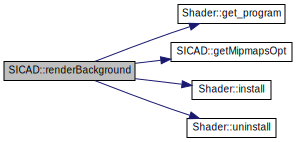
\includegraphics[width=350pt]{classSICAD_a46fcf7ddb480a788463a4d98d26e12e8_cgraph}
\end{center}
\end{figure}
\mbox{\Hypertarget{classSICAD_a07921943ad3d4016dcbe76135e799754}\label{classSICAD_a07921943ad3d4016dcbe76135e799754}} 
\index{S\+I\+C\+AD@{S\+I\+C\+AD}!set\+Background\+Opt@{set\+Background\+Opt}}
\index{set\+Background\+Opt@{set\+Background\+Opt}!S\+I\+C\+AD@{S\+I\+C\+AD}}
\subsubsection{\texorpdfstring{set\+Background\+Opt()}{setBackgroundOpt()}}
{\footnotesize\ttfamily void S\+I\+C\+A\+D\+::set\+Background\+Opt (\begin{DoxyParamCaption}\item[{bool}]{show\+\_\+background }\end{DoxyParamCaption})}



Definition at line 1291 of file S\+I\+C\+A\+D.\+cpp.



References show\+\_\+background\+\_\+.



Referenced by main().

\mbox{\Hypertarget{classSICAD_a1fa052a3609f52156b472e872e34971a}\label{classSICAD_a1fa052a3609f52156b472e872e34971a}} 
\index{S\+I\+C\+AD@{S\+I\+C\+AD}!set\+Mipmaps\+Opt@{set\+Mipmaps\+Opt}}
\index{set\+Mipmaps\+Opt@{set\+Mipmaps\+Opt}!S\+I\+C\+AD@{S\+I\+C\+AD}}
\subsubsection{\texorpdfstring{set\+Mipmaps\+Opt()}{setMipmapsOpt()}}
{\footnotesize\ttfamily void S\+I\+C\+A\+D\+::set\+Mipmaps\+Opt (\begin{DoxyParamCaption}\item[{const \mbox{\hyperlink{classSICAD_a7e092dede6f660355462d6d548214198}{M\+I\+P\+Maps}} \&}]{mipmaps }\end{DoxyParamCaption})}



Definition at line 1310 of file S\+I\+C\+A\+D.\+cpp.



References mesh\+\_\+mmaps\+\_\+.

\mbox{\Hypertarget{classSICAD_a0e42acab32252ddc878794f365ee1037}\label{classSICAD_a0e42acab32252ddc878794f365ee1037}} 
\index{S\+I\+C\+AD@{S\+I\+C\+AD}!set\+Ogl\+Window\+Should\+Close@{set\+Ogl\+Window\+Should\+Close}}
\index{set\+Ogl\+Window\+Should\+Close@{set\+Ogl\+Window\+Should\+Close}!S\+I\+C\+AD@{S\+I\+C\+AD}}
\subsubsection{\texorpdfstring{set\+Ogl\+Window\+Should\+Close()}{setOglWindowShouldClose()}}
{\footnotesize\ttfamily void S\+I\+C\+A\+D\+::set\+Ogl\+Window\+Should\+Close (\begin{DoxyParamCaption}\item[{bool}]{should\+\_\+close }\end{DoxyParamCaption})}



Definition at line 455 of file S\+I\+C\+A\+D.\+cpp.



References poll\+Or\+Post\+Event(), and window\+\_\+.

Here is the call graph for this function\+:\nopagebreak
\begin{figure}[H]
\begin{center}
\leavevmode
\includegraphics[width=350pt]{classSICAD_a0e42acab32252ddc878794f365ee1037_cgraph}
\end{center}
\end{figure}
\mbox{\Hypertarget{classSICAD_a39cdff6871d32429d8ba95b776e0b874}\label{classSICAD_a39cdff6871d32429d8ba95b776e0b874}} 
\index{S\+I\+C\+AD@{S\+I\+C\+AD}!set\+Projection\+Matrix@{set\+Projection\+Matrix}}
\index{set\+Projection\+Matrix@{set\+Projection\+Matrix}!S\+I\+C\+AD@{S\+I\+C\+AD}}
\subsubsection{\texorpdfstring{set\+Projection\+Matrix()}{setProjectionMatrix()}}
{\footnotesize\ttfamily bool S\+I\+C\+A\+D\+::set\+Projection\+Matrix (\begin{DoxyParamCaption}\item[{const G\+Lsizei}]{cam\+\_\+width,  }\item[{const G\+Lsizei}]{cam\+\_\+height,  }\item[{const G\+Lfloat}]{cam\+\_\+fx,  }\item[{const G\+Lfloat}]{cam\+\_\+fy,  }\item[{const G\+Lfloat}]{cam\+\_\+cx,  }\item[{const G\+Lfloat}]{cam\+\_\+cy }\end{DoxyParamCaption})}



Definition at line 1234 of file S\+I\+C\+A\+D.\+cpp.

\mbox{\Hypertarget{classSICAD_ae7af7aba5d81b9f1cc3e273a55811a70}\label{classSICAD_ae7af7aba5d81b9f1cc3e273a55811a70}} 
\index{S\+I\+C\+AD@{S\+I\+C\+AD}!set\+Wireframe@{set\+Wireframe}}
\index{set\+Wireframe@{set\+Wireframe}!S\+I\+C\+AD@{S\+I\+C\+AD}}
\subsubsection{\texorpdfstring{set\+Wireframe()}{setWireframe()}}
{\footnotesize\ttfamily void S\+I\+C\+A\+D\+::set\+Wireframe (\begin{DoxyParamCaption}\item[{G\+Lenum}]{mode }\end{DoxyParamCaption})\hspace{0.3cm}{\ttfamily [private]}}



Definition at line 1405 of file S\+I\+C\+A\+D.\+cpp.

\mbox{\Hypertarget{classSICAD_a4cf80a273b6b0d946cd298472c63ddd4}\label{classSICAD_a4cf80a273b6b0d946cd298472c63ddd4}} 
\index{S\+I\+C\+AD@{S\+I\+C\+AD}!set\+Wireframe\+Opt@{set\+Wireframe\+Opt}}
\index{set\+Wireframe\+Opt@{set\+Wireframe\+Opt}!S\+I\+C\+AD@{S\+I\+C\+AD}}
\subsubsection{\texorpdfstring{set\+Wireframe\+Opt()}{setWireframeOpt()}}
{\footnotesize\ttfamily void S\+I\+C\+A\+D\+::set\+Wireframe\+Opt (\begin{DoxyParamCaption}\item[{bool}]{show\+\_\+mesh\+\_\+wires }\end{DoxyParamCaption})}



Definition at line 1303 of file S\+I\+C\+A\+D.\+cpp.



References show\+\_\+mesh\+\_\+mode\+\_\+.

\mbox{\Hypertarget{classSICAD_a356e0ac8a0f130952a72326bedd4ab60}\label{classSICAD_a356e0ac8a0f130952a72326bedd4ab60}} 
\index{S\+I\+C\+AD@{S\+I\+C\+AD}!superimpose@{superimpose}}
\index{superimpose@{superimpose}!S\+I\+C\+AD@{S\+I\+C\+AD}}
\subsubsection{\texorpdfstring{superimpose()}{superimpose()}\hspace{0.1cm}{\footnotesize\ttfamily [1/8]}}
{\footnotesize\ttfamily bool S\+I\+C\+A\+D\+::superimpose (\begin{DoxyParamCaption}\item[{const \mbox{\hyperlink{classSuperimpose_a178e3d4e2def6635bfcf9454dd4b5d22}{Model\+Pose\+Container}} \&}]{objpos\+\_\+map,  }\item[{const double $\ast$}]{cam\+\_\+x,  }\item[{const double $\ast$}]{cam\+\_\+o,  }\item[{cv\+::\+Mat \&}]{img }\end{DoxyParamCaption})\hspace{0.3cm}{\ttfamily [override]}, {\ttfamily [virtual]}}



Render the mesh models in the pose specified in {\ttfamily objpos\+\_\+map} and move the virtual camera in {\ttfamily cam\+\_\+x} position with orientation {\ttfamily cam\+\_\+o}. 

The method then creates an image of the mesh models as they are seen by the virtual camera.

\begin{DoxyNote}{Note}
If cv\+::\+Mat {\ttfamily img} is a background image it must be of size {\ttfamily cam\+\_\+width $\ast$ cam\+\_\+height}, as specified during object construction, and the {\ttfamily \mbox{\hyperlink{classSICAD_a07921943ad3d4016dcbe76135e799754}{S\+I\+C\+A\+D\+::set\+Background\+Opt(bool show\+\_\+background)}}} must have been invoked with {\ttfamily true}.
\end{DoxyNote}

\begin{DoxyParams}{Parameters}
{\em objpos\+\_\+map} & A (tag, pose) container to associate a 7-\/component {\ttfamily pose}, (x, y, z) position and a (ux, uy, uz, theta) axis-\/angle orientation, to a mesh with tag \textquotesingle{}tag\textquotesingle{}. \\
\hline
{\em cam\+\_\+x} & (x, y, z) position. \\
\hline
{\em cam\+\_\+o} & (ux, uy, uz, theta) axis-\/angle orientation. \\
\hline
{\em img} & An image representing the result of the superimposition. The variable is automatically resized if its size is not correct to store the entire result of the superimposition.\\
\hline
\end{DoxyParams}
\begin{DoxyReturn}{Returns}
true upon success, false otherswise. 
\end{DoxyReturn}


Implements \mbox{\hyperlink{classSuperimpose_a62c4c269b8fc34cc36d3d54fa4acb35c}{Superimpose}}.



Definition at line 464 of file S\+I\+C\+A\+D.\+cpp.



Referenced by main().

\mbox{\Hypertarget{classSICAD_ab15f84cec5a65c8dd6cad85f9b0e1993}\label{classSICAD_ab15f84cec5a65c8dd6cad85f9b0e1993}} 
\index{S\+I\+C\+AD@{S\+I\+C\+AD}!superimpose@{superimpose}}
\index{superimpose@{superimpose}!S\+I\+C\+AD@{S\+I\+C\+AD}}
\subsubsection{\texorpdfstring{superimpose()}{superimpose()}\hspace{0.1cm}{\footnotesize\ttfamily [2/8]}}
{\footnotesize\ttfamily bool S\+I\+C\+A\+D\+::superimpose (\begin{DoxyParamCaption}\item[{const std\+::vector$<$ \mbox{\hyperlink{classSuperimpose_a178e3d4e2def6635bfcf9454dd4b5d22}{Model\+Pose\+Container}} $>$ \&}]{objpos\+\_\+multimap,  }\item[{const double $\ast$}]{cam\+\_\+x,  }\item[{const double $\ast$}]{cam\+\_\+o,  }\item[{cv\+::\+Mat \&}]{img }\end{DoxyParamCaption})\hspace{0.3cm}{\ttfamily [virtual]}}



Render the mesh models in the pose specified in each element of {\ttfamily objpos\+\_\+multimap} and move the virtual camera in {\ttfamily cam\+\_\+x} position with orientation {\ttfamily cam\+\_\+o}. 

Each group of meshes specified by the elements of {\ttfamily objpos\+\_\+multimap} are rendered in a different viewport. Each viewport reports the mesh models as they are seen by the virtual camera. The method then creates a single image tiling the viewports in a regular grid.

\begin{DoxyNote}{Note}
The size of the grid representing the tiled viewports can be accessed through {\ttfamily \mbox{\hyperlink{classSICAD_a9e3dd48dfd83ea0bd00d64dacc4fbd40}{get\+Tiles\+Rows()}}} and {\ttfamily \mbox{\hyperlink{classSICAD_a2ba3a0aeb3dab9996bdeed19a16eae56}{get\+Tiles\+Cols()}}}.

If cv\+::\+Mat {\ttfamily img} is a background image it must be of size {\ttfamily cam\+\_\+width $\ast$ cam\+\_\+height}, as specified during object construction, and the {\ttfamily \mbox{\hyperlink{classSICAD_a07921943ad3d4016dcbe76135e799754}{S\+I\+C\+A\+D\+::set\+Background\+Opt(bool show\+\_\+background)}}} must have been invoked with {\ttfamily true}.
\end{DoxyNote}

\begin{DoxyParams}{Parameters}
{\em objpos\+\_\+map} & A (tag, pose) container to associate a 7-\/component {\ttfamily pose}, (x, y, z) position and a (ux, uy, uz, theta) axis-\/angle orientation, to a mesh with tag \textquotesingle{}tag\textquotesingle{}. \\
\hline
{\em cam\+\_\+x} & (x, y, z) position. \\
\hline
{\em cam\+\_\+o} & (ux, uy, uz, theta) axis-\/angle orientation. \\
\hline
{\em img} & An image representing the result of the superimposition. The variable is automatically resized if its size is not correct to store the entire result of the superimposition.\\
\hline
\end{DoxyParams}
\begin{DoxyReturn}{Returns}
true upon success, false otherswise. 
\end{DoxyReturn}


Definition at line 576 of file S\+I\+C\+A\+D.\+cpp.

\mbox{\Hypertarget{classSICAD_af6c19a679de29992c5f9609f4424add0}\label{classSICAD_af6c19a679de29992c5f9609f4424add0}} 
\index{S\+I\+C\+AD@{S\+I\+C\+AD}!superimpose@{superimpose}}
\index{superimpose@{superimpose}!S\+I\+C\+AD@{S\+I\+C\+AD}}
\subsubsection{\texorpdfstring{superimpose()}{superimpose()}\hspace{0.1cm}{\footnotesize\ttfamily [3/8]}}
{\footnotesize\ttfamily bool S\+I\+C\+A\+D\+::superimpose (\begin{DoxyParamCaption}\item[{const \mbox{\hyperlink{classSuperimpose_a178e3d4e2def6635bfcf9454dd4b5d22}{Model\+Pose\+Container}} \&}]{objpos\+\_\+map,  }\item[{const double $\ast$}]{cam\+\_\+x,  }\item[{const double $\ast$}]{cam\+\_\+o,  }\item[{cv\+::\+Mat \&}]{img,  }\item[{const G\+Lsizei}]{cam\+\_\+width,  }\item[{const G\+Lsizei}]{cam\+\_\+height,  }\item[{const G\+Lfloat}]{cam\+\_\+fx,  }\item[{const G\+Lfloat}]{cam\+\_\+fy,  }\item[{const G\+Lfloat}]{cam\+\_\+cx,  }\item[{const G\+Lfloat}]{cam\+\_\+cy }\end{DoxyParamCaption})\hspace{0.3cm}{\ttfamily [virtual]}}



Definition at line 701 of file S\+I\+C\+A\+D.\+cpp.

\mbox{\Hypertarget{classSICAD_a269e238387393b44177daa4eae88fedd}\label{classSICAD_a269e238387393b44177daa4eae88fedd}} 
\index{S\+I\+C\+AD@{S\+I\+C\+AD}!superimpose@{superimpose}}
\index{superimpose@{superimpose}!S\+I\+C\+AD@{S\+I\+C\+AD}}
\subsubsection{\texorpdfstring{superimpose()}{superimpose()}\hspace{0.1cm}{\footnotesize\ttfamily [4/8]}}
{\footnotesize\ttfamily bool S\+I\+C\+A\+D\+::superimpose (\begin{DoxyParamCaption}\item[{const std\+::vector$<$ \mbox{\hyperlink{classSuperimpose_a178e3d4e2def6635bfcf9454dd4b5d22}{Model\+Pose\+Container}} $>$ \&}]{objpos\+\_\+multimap,  }\item[{const double $\ast$}]{cam\+\_\+x,  }\item[{const double $\ast$}]{cam\+\_\+o,  }\item[{cv\+::\+Mat \&}]{img,  }\item[{const G\+Lsizei}]{cam\+\_\+width,  }\item[{const G\+Lsizei}]{cam\+\_\+height,  }\item[{const G\+Lfloat}]{cam\+\_\+fx,  }\item[{const G\+Lfloat}]{cam\+\_\+fy,  }\item[{const G\+Lfloat}]{cam\+\_\+cx,  }\item[{const G\+Lfloat}]{cam\+\_\+cy }\end{DoxyParamCaption})\hspace{0.3cm}{\ttfamily [virtual]}}



Definition at line 722 of file S\+I\+C\+A\+D.\+cpp.

\mbox{\Hypertarget{classSICAD_a5a76058edfdeed2b37b40bde2eec3db1}\label{classSICAD_a5a76058edfdeed2b37b40bde2eec3db1}} 
\index{S\+I\+C\+AD@{S\+I\+C\+AD}!superimpose@{superimpose}}
\index{superimpose@{superimpose}!S\+I\+C\+AD@{S\+I\+C\+AD}}
\subsubsection{\texorpdfstring{superimpose()}{superimpose()}\hspace{0.1cm}{\footnotesize\ttfamily [5/8]}}
{\footnotesize\ttfamily bool S\+I\+C\+A\+D\+::superimpose (\begin{DoxyParamCaption}\item[{const \mbox{\hyperlink{classSuperimpose_a178e3d4e2def6635bfcf9454dd4b5d22}{Model\+Pose\+Container}} \&}]{objpos\+\_\+map,  }\item[{const double $\ast$}]{cam\+\_\+x,  }\item[{const double $\ast$}]{cam\+\_\+o,  }\item[{const size\+\_\+t}]{pbo\+\_\+index }\end{DoxyParamCaption})\hspace{0.3cm}{\ttfamily [virtual]}}



Render the mesh models in the pose specified in {\ttfamily objpos\+\_\+map} and move the virtual camera in {\ttfamily cam\+\_\+x} position with orientation {\ttfamily cam\+\_\+o}. 

The method then stores the pixels of the mesh models as they are seen by the virtual camera in the {\ttfamily pbo\+\_\+index}-\/th Pixel Buffer Object (P\+BO).

\begin{DoxyNote}{Note}
By invoking this command rendered pixels are stored in the {\ttfamily pbo\+\_\+index}-\/th P\+BO and, in order to use it, the Open\+GL context must remain current. As a consequence, once you are done working with the {\ttfamily pbo\+\_\+index}-\/th P\+BO (can be accessed by means of {\ttfamily S\+I\+C\+A\+D\+::get\+P\+B\+O(pbo\+\_\+index)}) and before invoking again any other {\ttfamily \mbox{\hyperlink{classSICAD_a356e0ac8a0f130952a72326bedd4ab60}{S\+I\+C\+A\+D\+::superimpose()}}} function, you must invoke {\ttfamily \mbox{\hyperlink{classSICAD_ae626fa7f8fd4dc5fc4bdc4f5311beede}{S\+I\+C\+A\+D\+::release\+Context()}}}.
\end{DoxyNote}

\begin{DoxyParams}{Parameters}
{\em objpos\+\_\+map} & A (tag, pose) container to associate a 7-\/component {\ttfamily pose}, (x, y, z) position and a (ux, uy, uz, theta) axis-\/angle orientation, to a mesh with tag \textquotesingle{}tag\textquotesingle{}. \\
\hline
{\em cam\+\_\+x} & (x, y, z) position. \\
\hline
{\em cam\+\_\+o} & (ux, uy, uz, theta) axis-\/angle orientation. \\
\hline
{\em pbo\+\_\+index} & The index of the P\+BO where the pixel are stored.\\
\hline
\end{DoxyParams}
\begin{DoxyReturn}{Returns}
(true, P\+BO) upon success, (false, 0) otherswise. 
\end{DoxyReturn}


Definition at line 743 of file S\+I\+C\+A\+D.\+cpp.

\mbox{\Hypertarget{classSICAD_a0dfbfdd508faf5f07a58ddfb6b9da50b}\label{classSICAD_a0dfbfdd508faf5f07a58ddfb6b9da50b}} 
\index{S\+I\+C\+AD@{S\+I\+C\+AD}!superimpose@{superimpose}}
\index{superimpose@{superimpose}!S\+I\+C\+AD@{S\+I\+C\+AD}}
\subsubsection{\texorpdfstring{superimpose()}{superimpose()}\hspace{0.1cm}{\footnotesize\ttfamily [6/8]}}
{\footnotesize\ttfamily bool S\+I\+C\+A\+D\+::superimpose (\begin{DoxyParamCaption}\item[{const \mbox{\hyperlink{classSuperimpose_a178e3d4e2def6635bfcf9454dd4b5d22}{Model\+Pose\+Container}} \&}]{objpos\+\_\+map,  }\item[{const double $\ast$}]{cam\+\_\+x,  }\item[{const double $\ast$}]{cam\+\_\+o,  }\item[{const size\+\_\+t}]{pbo\+\_\+index,  }\item[{const cv\+::\+Mat \&}]{img }\end{DoxyParamCaption})\hspace{0.3cm}{\ttfamily [virtual]}}



Render the mesh models in the pose specified in {\ttfamily objpos\+\_\+map} and move the virtual camera in {\ttfamily cam\+\_\+x} position with orientation {\ttfamily cam\+\_\+o}. 

The method then stores the pixels of the mesh models as they are seen by the virtual camera in the {\ttfamily pbo\+\_\+index}-\/th Pixel Buffer Object (P\+BO).

\begin{DoxyNote}{Note}
{\ttfamily img} must be of size {\ttfamily cam\+\_\+width $\ast$ cam\+\_\+height}, as specified during object construction, and the {\ttfamily \mbox{\hyperlink{classSICAD_a07921943ad3d4016dcbe76135e799754}{S\+I\+C\+A\+D\+::set\+Background\+Opt(bool show\+\_\+background)}}} must have been invoked with {\ttfamily true}.
\end{DoxyNote}

\begin{DoxyParams}{Parameters}
{\em objpos\+\_\+map} & A (tag, pose) container to associate a 7-\/component {\ttfamily pose}, (x, y, z) position and a (ux, uy, uz, theta) axis-\/angle orientation, to a mesh with tag \textquotesingle{}tag\textquotesingle{}. \\
\hline
{\em cam\+\_\+x} & (x, y, z) position. \\
\hline
{\em cam\+\_\+o} & (ux, uy, uz, theta) axis-\/angle orientation. \\
\hline
{\em pbo\+\_\+index} & The index of the P\+BO where the pixel are stored. \\
\hline
{\em img} & A background image.\\
\hline
\end{DoxyParams}
\begin{DoxyReturn}{Returns}
(true, P\+BO) upon success, (false, 0) otherswise. 
\end{DoxyReturn}


Definition at line 850 of file S\+I\+C\+A\+D.\+cpp.

\mbox{\Hypertarget{classSICAD_acf0ea95ecb121c0b265ca52ac589d80f}\label{classSICAD_acf0ea95ecb121c0b265ca52ac589d80f}} 
\index{S\+I\+C\+AD@{S\+I\+C\+AD}!superimpose@{superimpose}}
\index{superimpose@{superimpose}!S\+I\+C\+AD@{S\+I\+C\+AD}}
\subsubsection{\texorpdfstring{superimpose()}{superimpose()}\hspace{0.1cm}{\footnotesize\ttfamily [7/8]}}
{\footnotesize\ttfamily bool S\+I\+C\+A\+D\+::superimpose (\begin{DoxyParamCaption}\item[{const std\+::vector$<$ \mbox{\hyperlink{classSuperimpose_a178e3d4e2def6635bfcf9454dd4b5d22}{Model\+Pose\+Container}} $>$ \&}]{objpos\+\_\+multimap,  }\item[{const double $\ast$}]{cam\+\_\+x,  }\item[{const double $\ast$}]{cam\+\_\+o,  }\item[{const size\+\_\+t}]{pbo\+\_\+index }\end{DoxyParamCaption})\hspace{0.3cm}{\ttfamily [virtual]}}



Render the mesh models in the pose specified in each element of {\ttfamily objpos\+\_\+multimap} and move the virtual camera in {\ttfamily cam\+\_\+x} position with orientation {\ttfamily cam\+\_\+o}. 

Each group of meshes specified by the elements of {\ttfamily objpos\+\_\+multimap} are rendered in a different viewport. Each viewport reports the mesh models as they are seen by the virtual camera. The method then stores the pixels of the viewports in the {\ttfamily pbo\+\_\+index}-\/th Pixel Buffer Object (P\+BO) by tiling them in a regular grid.

\begin{DoxyNote}{Note}
By invoking this command rendered pixels are stored in the {\ttfamily pbo\+\_\+index}-\/th P\+BO and, in order to use it, the Open\+GL context must remain current. As a consequence, once you are done working with the {\ttfamily pbo\+\_\+index}-\/th P\+BO (can be accessed by means of {\ttfamily S\+I\+C\+A\+D\+::get\+P\+B\+O(pbo\+\_\+index)}) and before invoking again any other {\ttfamily \mbox{\hyperlink{classSICAD_a356e0ac8a0f130952a72326bedd4ab60}{S\+I\+C\+A\+D\+::superimpose()}}} function, you must invoke {\ttfamily \mbox{\hyperlink{classSICAD_ae626fa7f8fd4dc5fc4bdc4f5311beede}{S\+I\+C\+A\+D\+::release\+Context()}}}.

The size of the grid representing the tiled viewports can be accessed through {\ttfamily \mbox{\hyperlink{classSICAD_a9e3dd48dfd83ea0bd00d64dacc4fbd40}{get\+Tiles\+Rows()}}} and {\ttfamily \mbox{\hyperlink{classSICAD_a2ba3a0aeb3dab9996bdeed19a16eae56}{get\+Tiles\+Cols()}}}.
\end{DoxyNote}

\begin{DoxyParams}{Parameters}
{\em objpos\+\_\+map} & A (tag, pose) container to associate a 7-\/component {\ttfamily pose}, (x, y, z) position and a (ux, uy, uz, theta) axis-\/angle orientation, to a mesh with tag \textquotesingle{}tag\textquotesingle{}. \\
\hline
{\em cam\+\_\+x} & (x, y, z) position. \\
\hline
{\em cam\+\_\+o} & (ux, uy, uz, theta) axis-\/angle orientation. \\
\hline
{\em pbo\+\_\+index} & The index of the P\+BO where the pixel are stored.\\
\hline
\end{DoxyParams}
\begin{DoxyReturn}{Returns}
(true, P\+BO) upon success, (false, 0) otherswise. 
\end{DoxyReturn}


Definition at line 962 of file S\+I\+C\+A\+D.\+cpp.

\mbox{\Hypertarget{classSICAD_a264db68e6189b5907d162947267be056}\label{classSICAD_a264db68e6189b5907d162947267be056}} 
\index{S\+I\+C\+AD@{S\+I\+C\+AD}!superimpose@{superimpose}}
\index{superimpose@{superimpose}!S\+I\+C\+AD@{S\+I\+C\+AD}}
\subsubsection{\texorpdfstring{superimpose()}{superimpose()}\hspace{0.1cm}{\footnotesize\ttfamily [8/8]}}
{\footnotesize\ttfamily bool S\+I\+C\+A\+D\+::superimpose (\begin{DoxyParamCaption}\item[{const std\+::vector$<$ \mbox{\hyperlink{classSuperimpose_a178e3d4e2def6635bfcf9454dd4b5d22}{Model\+Pose\+Container}} $>$ \&}]{objpos\+\_\+multimap,  }\item[{const double $\ast$}]{cam\+\_\+x,  }\item[{const double $\ast$}]{cam\+\_\+o,  }\item[{const size\+\_\+t}]{pbo\+\_\+index,  }\item[{const cv\+::\+Mat \&}]{img }\end{DoxyParamCaption})\hspace{0.3cm}{\ttfamily [virtual]}}



Render the mesh models in the pose specified in each element of {\ttfamily objpos\+\_\+multimap} and move the virtual camera in {\ttfamily cam\+\_\+x} position with orientation {\ttfamily cam\+\_\+o}. 

Each group of meshes specified by the elements of {\ttfamily objpos\+\_\+multimap} are rendered in a different viewport. Each viewport reports the mesh models as they are seen by the virtual camera. The method then stores the pixels of the viewports in the {\ttfamily pbo\+\_\+index}-\/th Pixel Buffer Object (P\+BO) by tiling them in a regular grid.

\begin{DoxyNote}{Note}
The size of the grid representing the tiled viewports can be accessed through {\ttfamily \mbox{\hyperlink{classSICAD_a9e3dd48dfd83ea0bd00d64dacc4fbd40}{get\+Tiles\+Rows()}}} and {\ttfamily \mbox{\hyperlink{classSICAD_a2ba3a0aeb3dab9996bdeed19a16eae56}{get\+Tiles\+Cols()}}}.

{\ttfamily img} must be of size {\ttfamily cam\+\_\+width $\ast$ cam\+\_\+height}, as specified during object construction, and the {\ttfamily \mbox{\hyperlink{classSICAD_a07921943ad3d4016dcbe76135e799754}{S\+I\+C\+A\+D\+::set\+Background\+Opt(bool show\+\_\+background)}}} must have been invoked with {\ttfamily true}.
\end{DoxyNote}

\begin{DoxyParams}{Parameters}
{\em objpos\+\_\+map} & A (tag, pose) container to associate a 7-\/component {\ttfamily pose}, (x, y, z) position and a (ux, uy, uz, theta) axis-\/angle orientation, to a mesh with tag \textquotesingle{}tag\textquotesingle{}. \\
\hline
{\em cam\+\_\+x} & (x, y, z) position. \\
\hline
{\em cam\+\_\+o} & (ux, uy, uz, theta) axis-\/angle orientation. \\
\hline
{\em pbo\+\_\+index} & The index of the P\+BO where the pixel are stored. \\
\hline
{\em img} & A background image.\\
\hline
\end{DoxyParams}
\begin{DoxyReturn}{Returns}
(true, P\+BO) upon success, (false, 0) otherswise. 
\end{DoxyReturn}


Definition at line 1082 of file S\+I\+C\+A\+D.\+cpp.



\subsection{Member Data Documentation}
\mbox{\Hypertarget{classSICAD_ad5945f84df0d90113a24b2001ecbc832}\label{classSICAD_ad5945f84df0d90113a24b2001ecbc832}} 
\index{S\+I\+C\+AD@{S\+I\+C\+AD}!back\+\_\+proj\+\_\+@{back\+\_\+proj\+\_\+}}
\index{back\+\_\+proj\+\_\+@{back\+\_\+proj\+\_\+}!S\+I\+C\+AD@{S\+I\+C\+AD}}
\subsubsection{\texorpdfstring{back\+\_\+proj\+\_\+}{back\_proj\_}}
{\footnotesize\ttfamily glm\+::mat4 S\+I\+C\+A\+D\+::back\+\_\+proj\+\_\+\hspace{0.3cm}{\ttfamily [private]}}



Definition at line 404 of file S\+I\+C\+A\+D.\+h.



Referenced by render\+Background().

\mbox{\Hypertarget{classSICAD_a16f7c3c77ddea5ba57bbcbcdd7a8d125}\label{classSICAD_a16f7c3c77ddea5ba57bbcbcdd7a8d125}} 
\index{S\+I\+C\+AD@{S\+I\+C\+AD}!class\+\_\+counter\+\_\+@{class\+\_\+counter\+\_\+}}
\index{class\+\_\+counter\+\_\+@{class\+\_\+counter\+\_\+}!S\+I\+C\+AD@{S\+I\+C\+AD}}
\subsubsection{\texorpdfstring{class\+\_\+counter\+\_\+}{class\_counter\_}}
{\footnotesize\ttfamily int S\+I\+C\+A\+D\+::class\+\_\+counter\+\_\+ = 0\hspace{0.3cm}{\ttfamily [static]}, {\ttfamily [private]}}



Definition at line 332 of file S\+I\+C\+A\+D.\+h.



Referenced by $\sim$\+S\+I\+C\+A\+D().

\mbox{\Hypertarget{classSICAD_a2cdcd11dd55a4b02b85d7c32435cc719}\label{classSICAD_a2cdcd11dd55a4b02b85d7c32435cc719}} 
\index{S\+I\+C\+AD@{S\+I\+C\+AD}!ebo\+\_\+background\+\_\+@{ebo\+\_\+background\+\_\+}}
\index{ebo\+\_\+background\+\_\+@{ebo\+\_\+background\+\_\+}!S\+I\+C\+AD@{S\+I\+C\+AD}}
\subsubsection{\texorpdfstring{ebo\+\_\+background\+\_\+}{ebo\_background\_}}
{\footnotesize\ttfamily G\+Luint S\+I\+C\+A\+D\+::ebo\+\_\+background\+\_\+\hspace{0.3cm}{\ttfamily [private]}}



Definition at line 392 of file S\+I\+C\+A\+D.\+h.



Referenced by $\sim$\+S\+I\+C\+A\+D().

\mbox{\Hypertarget{classSICAD_a4c4d2e249ac824528e1fe9f97fa207d9}\label{classSICAD_a4c4d2e249ac824528e1fe9f97fa207d9}} 
\index{S\+I\+C\+AD@{S\+I\+C\+AD}!far\+\_\+@{far\+\_\+}}
\index{far\+\_\+@{far\+\_\+}!S\+I\+C\+AD@{S\+I\+C\+AD}}
\subsubsection{\texorpdfstring{far\+\_\+}{far\_}}
{\footnotesize\ttfamily const G\+Lfloat S\+I\+C\+A\+D\+::far\+\_\+ = 1000.\+0f\hspace{0.3cm}{\ttfamily [private]}}



Definition at line 362 of file S\+I\+C\+A\+D.\+h.

\mbox{\Hypertarget{classSICAD_a2c173ad18d42e090b46a539f92f3fe9d}\label{classSICAD_a2c173ad18d42e090b46a539f92f3fe9d}} 
\index{S\+I\+C\+AD@{S\+I\+C\+AD}!fbo\+\_\+@{fbo\+\_\+}}
\index{fbo\+\_\+@{fbo\+\_\+}!S\+I\+C\+AD@{S\+I\+C\+AD}}
\subsubsection{\texorpdfstring{fbo\+\_\+}{fbo\_}}
{\footnotesize\ttfamily G\+Luint S\+I\+C\+A\+D\+::fbo\+\_\+\hspace{0.3cm}{\ttfamily [private]}}



Definition at line 382 of file S\+I\+C\+A\+D.\+h.



Referenced by $\sim$\+S\+I\+C\+A\+D().

\mbox{\Hypertarget{classSICAD_a3361bb03e52bc0554bb1e3670ef3a0f9}\label{classSICAD_a3361bb03e52bc0554bb1e3670ef3a0f9}} 
\index{S\+I\+C\+AD@{S\+I\+C\+AD}!framebuffer\+\_\+height\+\_\+@{framebuffer\+\_\+height\+\_\+}}
\index{framebuffer\+\_\+height\+\_\+@{framebuffer\+\_\+height\+\_\+}!S\+I\+C\+AD@{S\+I\+C\+AD}}
\subsubsection{\texorpdfstring{framebuffer\+\_\+height\+\_\+}{framebuffer\_height\_}}
{\footnotesize\ttfamily G\+Lsizei S\+I\+C\+A\+D\+::framebuffer\+\_\+height\+\_\+ = 0\hspace{0.3cm}{\ttfamily [private]}}



Definition at line 354 of file S\+I\+C\+A\+D.\+h.

\mbox{\Hypertarget{classSICAD_a08c86b826a1784b132bac3f0792fc604}\label{classSICAD_a08c86b826a1784b132bac3f0792fc604}} 
\index{S\+I\+C\+AD@{S\+I\+C\+AD}!framebuffer\+\_\+width\+\_\+@{framebuffer\+\_\+width\+\_\+}}
\index{framebuffer\+\_\+width\+\_\+@{framebuffer\+\_\+width\+\_\+}!S\+I\+C\+AD@{S\+I\+C\+AD}}
\subsubsection{\texorpdfstring{framebuffer\+\_\+width\+\_\+}{framebuffer\_width\_}}
{\footnotesize\ttfamily G\+Lsizei S\+I\+C\+A\+D\+::framebuffer\+\_\+width\+\_\+ = 0\hspace{0.3cm}{\ttfamily [private]}}



Definition at line 352 of file S\+I\+C\+A\+D.\+h.

\mbox{\Hypertarget{classSICAD_a093da94bc84a46d08f71051c4d88c176}\label{classSICAD_a093da94bc84a46d08f71051c4d88c176}} 
\index{S\+I\+C\+AD@{S\+I\+C\+AD}!image\+\_\+height\+\_\+@{image\+\_\+height\+\_\+}}
\index{image\+\_\+height\+\_\+@{image\+\_\+height\+\_\+}!S\+I\+C\+AD@{S\+I\+C\+AD}}
\subsubsection{\texorpdfstring{image\+\_\+height\+\_\+}{image\_height\_}}
{\footnotesize\ttfamily G\+Lsizei S\+I\+C\+A\+D\+::image\+\_\+height\+\_\+ = 0\hspace{0.3cm}{\ttfamily [private]}}



Definition at line 348 of file S\+I\+C\+A\+D.\+h.

\mbox{\Hypertarget{classSICAD_ade37d5c3960d164acaa749745f55070f}\label{classSICAD_ade37d5c3960d164acaa749745f55070f}} 
\index{S\+I\+C\+AD@{S\+I\+C\+AD}!image\+\_\+width\+\_\+@{image\+\_\+width\+\_\+}}
\index{image\+\_\+width\+\_\+@{image\+\_\+width\+\_\+}!S\+I\+C\+AD@{S\+I\+C\+AD}}
\subsubsection{\texorpdfstring{image\+\_\+width\+\_\+}{image\_width\_}}
{\footnotesize\ttfamily G\+Lsizei S\+I\+C\+A\+D\+::image\+\_\+width\+\_\+ = 0\hspace{0.3cm}{\ttfamily [private]}}



Definition at line 346 of file S\+I\+C\+A\+D.\+h.

\mbox{\Hypertarget{classSICAD_a9eb34b659cac13b8442ca821455cc1f1}\label{classSICAD_a9eb34b659cac13b8442ca821455cc1f1}} 
\index{S\+I\+C\+AD@{S\+I\+C\+AD}!log\+\_\+\+I\+D\+\_\+@{log\+\_\+\+I\+D\+\_\+}}
\index{log\+\_\+\+I\+D\+\_\+@{log\+\_\+\+I\+D\+\_\+}!S\+I\+C\+AD@{S\+I\+C\+AD}}
\subsubsection{\texorpdfstring{log\+\_\+\+I\+D\+\_\+}{log\_ID\_}}
{\footnotesize\ttfamily const std\+::string S\+I\+C\+A\+D\+::log\+\_\+\+I\+D\+\_\+ = \char`\"{}\mbox{[}S\+I\+::\+S\+I\+C\+AD\mbox{]}\char`\"{}\hspace{0.3cm}{\ttfamily [private]}}



Definition at line 336 of file S\+I\+C\+A\+D.\+h.



Referenced by $\sim$\+S\+I\+C\+A\+D().

\mbox{\Hypertarget{classSICAD_a6a4623d27b2ee48ad0db90bd075c708c}\label{classSICAD_a6a4623d27b2ee48ad0db90bd075c708c}} 
\index{S\+I\+C\+AD@{S\+I\+C\+AD}!main\+\_\+thread\+\_\+id\+\_\+@{main\+\_\+thread\+\_\+id\+\_\+}}
\index{main\+\_\+thread\+\_\+id\+\_\+@{main\+\_\+thread\+\_\+id\+\_\+}!S\+I\+C\+AD@{S\+I\+C\+AD}}
\subsubsection{\texorpdfstring{main\+\_\+thread\+\_\+id\+\_\+}{main\_thread\_id\_}}
{\footnotesize\ttfamily std\+::thread\+::id S\+I\+C\+A\+D\+::main\+\_\+thread\+\_\+id\+\_\+\hspace{0.3cm}{\ttfamily [private]}}



Definition at line 364 of file S\+I\+C\+A\+D.\+h.



Referenced by poll\+Or\+Post\+Event().

\mbox{\Hypertarget{classSICAD_a34b0de96321855145937cc5858c019b0}\label{classSICAD_a34b0de96321855145937cc5858c019b0}} 
\index{S\+I\+C\+AD@{S\+I\+C\+AD}!mesh\+\_\+mmaps\+\_\+@{mesh\+\_\+mmaps\+\_\+}}
\index{mesh\+\_\+mmaps\+\_\+@{mesh\+\_\+mmaps\+\_\+}!S\+I\+C\+AD@{S\+I\+C\+AD}}
\subsubsection{\texorpdfstring{mesh\+\_\+mmaps\+\_\+}{mesh\_mmaps\_}}
{\footnotesize\ttfamily \mbox{\hyperlink{classSICAD_a7e092dede6f660355462d6d548214198}{M\+I\+P\+Maps}} S\+I\+C\+A\+D\+::mesh\+\_\+mmaps\+\_\+ = \mbox{\hyperlink{classSICAD_a7e092dede6f660355462d6d548214198ad879c351426770bc0b13c3628db1e636}{M\+I\+P\+Maps\+::nearest}}\hspace{0.3cm}{\ttfamily [private]}}



Definition at line 370 of file S\+I\+C\+A\+D.\+h.



Referenced by get\+Mipmaps\+Opt(), and set\+Mipmaps\+Opt().

\mbox{\Hypertarget{classSICAD_a05fea2b5b027a3b7f37ef9ea4ecd64f0}\label{classSICAD_a05fea2b5b027a3b7f37ef9ea4ecd64f0}} 
\index{S\+I\+C\+AD@{S\+I\+C\+AD}!model\+\_\+obj\+\_\+@{model\+\_\+obj\+\_\+}}
\index{model\+\_\+obj\+\_\+@{model\+\_\+obj\+\_\+}!S\+I\+C\+AD@{S\+I\+C\+AD}}
\subsubsection{\texorpdfstring{model\+\_\+obj\+\_\+}{model\_obj\_}}
{\footnotesize\ttfamily \mbox{\hyperlink{classSICAD_aca3c9693d298f2e8dc171194c6a7507c}{Model\+Container}} S\+I\+C\+A\+D\+::model\+\_\+obj\+\_\+\hspace{0.3cm}{\ttfamily [private]}}



Definition at line 380 of file S\+I\+C\+A\+D.\+h.



Referenced by $\sim$\+S\+I\+C\+A\+D().

\mbox{\Hypertarget{classSICAD_a690437655965101bad97d32e98015dd5}\label{classSICAD_a690437655965101bad97d32e98015dd5}} 
\index{S\+I\+C\+AD@{S\+I\+C\+AD}!near\+\_\+@{near\+\_\+}}
\index{near\+\_\+@{near\+\_\+}!S\+I\+C\+AD@{S\+I\+C\+AD}}
\subsubsection{\texorpdfstring{near\+\_\+}{near\_}}
{\footnotesize\ttfamily const G\+Lfloat S\+I\+C\+A\+D\+::near\+\_\+ = 0.\+001f\hspace{0.3cm}{\ttfamily [private]}}



Definition at line 360 of file S\+I\+C\+A\+D.\+h.

\mbox{\Hypertarget{classSICAD_a95af2758122e6420369516fd13fd03cc}\label{classSICAD_a95af2758122e6420369516fd13fd03cc}} 
\index{S\+I\+C\+AD@{S\+I\+C\+AD}!ogl\+\_\+to\+\_\+cam\+\_\+@{ogl\+\_\+to\+\_\+cam\+\_\+}}
\index{ogl\+\_\+to\+\_\+cam\+\_\+@{ogl\+\_\+to\+\_\+cam\+\_\+}!S\+I\+C\+AD@{S\+I\+C\+AD}}
\subsubsection{\texorpdfstring{ogl\+\_\+to\+\_\+cam\+\_\+}{ogl\_to\_cam\_}}
{\footnotesize\ttfamily glm\+::mat3 S\+I\+C\+A\+D\+::ogl\+\_\+to\+\_\+cam\+\_\+ = glm\+::mat3(1.\+0f)\hspace{0.3cm}{\ttfamily [private]}}



Definition at line 350 of file S\+I\+C\+A\+D.\+h.



Referenced by get\+View\+Transformation\+Matrix().

\mbox{\Hypertarget{classSICAD_a56b765675245d3b4501cfda799d4630a}\label{classSICAD_a56b765675245d3b4501cfda799d4630a}} 
\index{S\+I\+C\+AD@{S\+I\+C\+AD}!pbo\+\_\+@{pbo\+\_\+}}
\index{pbo\+\_\+@{pbo\+\_\+}!S\+I\+C\+AD@{S\+I\+C\+AD}}
\subsubsection{\texorpdfstring{pbo\+\_\+}{pbo\_}}
{\footnotesize\ttfamily G\+Luint S\+I\+C\+A\+D\+::pbo\+\_\+\mbox{[}2\mbox{]}\hspace{0.3cm}{\ttfamily [private]}}



Definition at line 402 of file S\+I\+C\+A\+D.\+h.



Referenced by get\+P\+B\+O(), get\+P\+B\+Os(), and $\sim$\+S\+I\+C\+A\+D().

\mbox{\Hypertarget{classSICAD_a3d7e1e1b3049508ea3c40b85541ea818}\label{classSICAD_a3d7e1e1b3049508ea3c40b85541ea818}} 
\index{S\+I\+C\+AD@{S\+I\+C\+AD}!pbo\+\_\+number\+\_\+@{pbo\+\_\+number\+\_\+}}
\index{pbo\+\_\+number\+\_\+@{pbo\+\_\+number\+\_\+}!S\+I\+C\+AD@{S\+I\+C\+AD}}
\subsubsection{\texorpdfstring{pbo\+\_\+number\+\_\+}{pbo\_number\_}}
{\footnotesize\ttfamily size\+\_\+t S\+I\+C\+A\+D\+::pbo\+\_\+number\+\_\+ = 2\hspace{0.3cm}{\ttfamily [private]}}



Definition at line 400 of file S\+I\+C\+A\+D.\+h.



Referenced by get\+P\+B\+O(), and get\+P\+B\+Os().

\mbox{\Hypertarget{classSICAD_afb91b682fd1f6629f163ab321869e7e0}\label{classSICAD_afb91b682fd1f6629f163ab321869e7e0}} 
\index{S\+I\+C\+AD@{S\+I\+C\+AD}!projection\+\_\+@{projection\+\_\+}}
\index{projection\+\_\+@{projection\+\_\+}!S\+I\+C\+AD@{S\+I\+C\+AD}}
\subsubsection{\texorpdfstring{projection\+\_\+}{projection\_}}
{\footnotesize\ttfamily glm\+::mat4 S\+I\+C\+A\+D\+::projection\+\_\+\hspace{0.3cm}{\ttfamily [private]}}



Definition at line 406 of file S\+I\+C\+A\+D.\+h.

\mbox{\Hypertarget{classSICAD_aca24504d58ce97106dbc95925f36fca0}\label{classSICAD_aca24504d58ce97106dbc95925f36fca0}} 
\index{S\+I\+C\+AD@{S\+I\+C\+AD}!renderbuffer\+\_\+size\+\_\+@{renderbuffer\+\_\+size\+\_\+}}
\index{renderbuffer\+\_\+size\+\_\+@{renderbuffer\+\_\+size\+\_\+}!S\+I\+C\+AD@{S\+I\+C\+AD}}
\subsubsection{\texorpdfstring{renderbuffer\+\_\+size\+\_\+}{renderbuffer\_size\_}}
{\footnotesize\ttfamily G\+Lsizei S\+I\+C\+A\+D\+::renderbuffer\+\_\+size\+\_\+ = 0\hspace{0.3cm}{\ttfamily [static]}, {\ttfamily [private]}}



Definition at line 334 of file S\+I\+C\+A\+D.\+h.

\mbox{\Hypertarget{classSICAD_a46edf33acc9f7ea3bd98c7ee6388ce9c}\label{classSICAD_a46edf33acc9f7ea3bd98c7ee6388ce9c}} 
\index{S\+I\+C\+AD@{S\+I\+C\+AD}!shader\+\_\+background\+\_\+@{shader\+\_\+background\+\_\+}}
\index{shader\+\_\+background\+\_\+@{shader\+\_\+background\+\_\+}!S\+I\+C\+AD@{S\+I\+C\+AD}}
\subsubsection{\texorpdfstring{shader\+\_\+background\+\_\+}{shader\_background\_}}
{\footnotesize\ttfamily \mbox{\hyperlink{classShader}{Shader}}$\ast$ S\+I\+C\+A\+D\+::shader\+\_\+background\+\_\+ = nullptr\hspace{0.3cm}{\ttfamily [private]}}



Definition at line 372 of file S\+I\+C\+A\+D.\+h.



Referenced by render\+Background(), and $\sim$\+S\+I\+C\+A\+D().

\mbox{\Hypertarget{classSICAD_a6c11f0e8dc8cbdd91748c230fc680833}\label{classSICAD_a6c11f0e8dc8cbdd91748c230fc680833}} 
\index{S\+I\+C\+AD@{S\+I\+C\+AD}!shader\+\_\+cad\+\_\+@{shader\+\_\+cad\+\_\+}}
\index{shader\+\_\+cad\+\_\+@{shader\+\_\+cad\+\_\+}!S\+I\+C\+AD@{S\+I\+C\+AD}}
\subsubsection{\texorpdfstring{shader\+\_\+cad\+\_\+}{shader\_cad\_}}
{\footnotesize\ttfamily \mbox{\hyperlink{classShader}{Shader}}$\ast$ S\+I\+C\+A\+D\+::shader\+\_\+cad\+\_\+ = nullptr\hspace{0.3cm}{\ttfamily [private]}}



Definition at line 374 of file S\+I\+C\+A\+D.\+h.



Referenced by $\sim$\+S\+I\+C\+A\+D().

\mbox{\Hypertarget{classSICAD_ac921e60623f3797253bcbcdd445b903b}\label{classSICAD_ac921e60623f3797253bcbcdd445b903b}} 
\index{S\+I\+C\+AD@{S\+I\+C\+AD}!shader\+\_\+frame\+\_\+@{shader\+\_\+frame\+\_\+}}
\index{shader\+\_\+frame\+\_\+@{shader\+\_\+frame\+\_\+}!S\+I\+C\+AD@{S\+I\+C\+AD}}
\subsubsection{\texorpdfstring{shader\+\_\+frame\+\_\+}{shader\_frame\_}}
{\footnotesize\ttfamily \mbox{\hyperlink{classShader}{Shader}}$\ast$ S\+I\+C\+A\+D\+::shader\+\_\+frame\+\_\+ = nullptr\hspace{0.3cm}{\ttfamily [private]}}



Definition at line 378 of file S\+I\+C\+A\+D.\+h.



Referenced by $\sim$\+S\+I\+C\+A\+D().

\mbox{\Hypertarget{classSICAD_aa9c575d7847080ed891015f457a8fd59}\label{classSICAD_aa9c575d7847080ed891015f457a8fd59}} 
\index{S\+I\+C\+AD@{S\+I\+C\+AD}!shader\+\_\+mesh\+\_\+texture\+\_\+@{shader\+\_\+mesh\+\_\+texture\+\_\+}}
\index{shader\+\_\+mesh\+\_\+texture\+\_\+@{shader\+\_\+mesh\+\_\+texture\+\_\+}!S\+I\+C\+AD@{S\+I\+C\+AD}}
\subsubsection{\texorpdfstring{shader\+\_\+mesh\+\_\+texture\+\_\+}{shader\_mesh\_texture\_}}
{\footnotesize\ttfamily std\+::unique\+\_\+ptr$<$\mbox{\hyperlink{classShader}{Shader}}$>$ S\+I\+C\+A\+D\+::shader\+\_\+mesh\+\_\+texture\+\_\+\hspace{0.3cm}{\ttfamily [private]}}



Definition at line 376 of file S\+I\+C\+A\+D.\+h.

\mbox{\Hypertarget{classSICAD_a8db9e37d71a14883be4879e9ea4b6a02}\label{classSICAD_a8db9e37d71a14883be4879e9ea4b6a02}} 
\index{S\+I\+C\+AD@{S\+I\+C\+AD}!show\+\_\+background\+\_\+@{show\+\_\+background\+\_\+}}
\index{show\+\_\+background\+\_\+@{show\+\_\+background\+\_\+}!S\+I\+C\+AD@{S\+I\+C\+AD}}
\subsubsection{\texorpdfstring{show\+\_\+background\+\_\+}{show\_background\_}}
{\footnotesize\ttfamily bool S\+I\+C\+A\+D\+::show\+\_\+background\+\_\+ = false\hspace{0.3cm}{\ttfamily [private]}}



Definition at line 366 of file S\+I\+C\+A\+D.\+h.



Referenced by get\+Background\+Opt(), and set\+Background\+Opt().

\mbox{\Hypertarget{classSICAD_a9c4c3ba5d071f763ee1956fa31faa3f8}\label{classSICAD_a9c4c3ba5d071f763ee1956fa31faa3f8}} 
\index{S\+I\+C\+AD@{S\+I\+C\+AD}!show\+\_\+mesh\+\_\+mode\+\_\+@{show\+\_\+mesh\+\_\+mode\+\_\+}}
\index{show\+\_\+mesh\+\_\+mode\+\_\+@{show\+\_\+mesh\+\_\+mode\+\_\+}!S\+I\+C\+AD@{S\+I\+C\+AD}}
\subsubsection{\texorpdfstring{show\+\_\+mesh\+\_\+mode\+\_\+}{show\_mesh\_mode\_}}
{\footnotesize\ttfamily G\+Lenum S\+I\+C\+A\+D\+::show\+\_\+mesh\+\_\+mode\+\_\+ = G\+L\+\_\+\+F\+I\+LL\hspace{0.3cm}{\ttfamily [private]}}



Definition at line 368 of file S\+I\+C\+A\+D.\+h.



Referenced by get\+Wireframe\+Opt(), and set\+Wireframe\+Opt().

\mbox{\Hypertarget{classSICAD_a2728fb0fa0be11f0992bc81b4873da4f}\label{classSICAD_a2728fb0fa0be11f0992bc81b4873da4f}} 
\index{S\+I\+C\+AD@{S\+I\+C\+AD}!texture\+\_\+background\+\_\+@{texture\+\_\+background\+\_\+}}
\index{texture\+\_\+background\+\_\+@{texture\+\_\+background\+\_\+}!S\+I\+C\+AD@{S\+I\+C\+AD}}
\subsubsection{\texorpdfstring{texture\+\_\+background\+\_\+}{texture\_background\_}}
{\footnotesize\ttfamily G\+Luint S\+I\+C\+A\+D\+::texture\+\_\+background\+\_\+\hspace{0.3cm}{\ttfamily [private]}}



Definition at line 388 of file S\+I\+C\+A\+D.\+h.



Referenced by render\+Background(), and $\sim$\+S\+I\+C\+A\+D().

\mbox{\Hypertarget{classSICAD_a50f1ec3b2545ca40d58466735da80fc6}\label{classSICAD_a50f1ec3b2545ca40d58466735da80fc6}} 
\index{S\+I\+C\+AD@{S\+I\+C\+AD}!texture\+\_\+color\+\_\+buffer\+\_\+@{texture\+\_\+color\+\_\+buffer\+\_\+}}
\index{texture\+\_\+color\+\_\+buffer\+\_\+@{texture\+\_\+color\+\_\+buffer\+\_\+}!S\+I\+C\+AD@{S\+I\+C\+AD}}
\subsubsection{\texorpdfstring{texture\+\_\+color\+\_\+buffer\+\_\+}{texture\_color\_buffer\_}}
{\footnotesize\ttfamily G\+Luint S\+I\+C\+A\+D\+::texture\+\_\+color\+\_\+buffer\+\_\+\hspace{0.3cm}{\ttfamily [private]}}



Definition at line 384 of file S\+I\+C\+A\+D.\+h.



Referenced by $\sim$\+S\+I\+C\+A\+D().

\mbox{\Hypertarget{classSICAD_a2fed5ac56bb2206fe8f6eccc9d784015}\label{classSICAD_a2fed5ac56bb2206fe8f6eccc9d784015}} 
\index{S\+I\+C\+AD@{S\+I\+C\+AD}!texture\+\_\+depth\+\_\+buffer\+\_\+@{texture\+\_\+depth\+\_\+buffer\+\_\+}}
\index{texture\+\_\+depth\+\_\+buffer\+\_\+@{texture\+\_\+depth\+\_\+buffer\+\_\+}!S\+I\+C\+AD@{S\+I\+C\+AD}}
\subsubsection{\texorpdfstring{texture\+\_\+depth\+\_\+buffer\+\_\+}{texture\_depth\_buffer\_}}
{\footnotesize\ttfamily G\+Luint S\+I\+C\+A\+D\+::texture\+\_\+depth\+\_\+buffer\+\_\+\hspace{0.3cm}{\ttfamily [private]}}



Definition at line 386 of file S\+I\+C\+A\+D.\+h.



Referenced by $\sim$\+S\+I\+C\+A\+D().

\mbox{\Hypertarget{classSICAD_a2e6b01258527769e4066262ed002fc69}\label{classSICAD_a2e6b01258527769e4066262ed002fc69}} 
\index{S\+I\+C\+AD@{S\+I\+C\+AD}!tile\+\_\+img\+\_\+height\+\_\+@{tile\+\_\+img\+\_\+height\+\_\+}}
\index{tile\+\_\+img\+\_\+height\+\_\+@{tile\+\_\+img\+\_\+height\+\_\+}!S\+I\+C\+AD@{S\+I\+C\+AD}}
\subsubsection{\texorpdfstring{tile\+\_\+img\+\_\+height\+\_\+}{tile\_img\_height\_}}
{\footnotesize\ttfamily G\+Lsizei S\+I\+C\+A\+D\+::tile\+\_\+img\+\_\+height\+\_\+ = 0\hspace{0.3cm}{\ttfamily [private]}}



Definition at line 358 of file S\+I\+C\+A\+D.\+h.

\mbox{\Hypertarget{classSICAD_a1dda156a616e004de5364914d8d6c4b9}\label{classSICAD_a1dda156a616e004de5364914d8d6c4b9}} 
\index{S\+I\+C\+AD@{S\+I\+C\+AD}!tile\+\_\+img\+\_\+width\+\_\+@{tile\+\_\+img\+\_\+width\+\_\+}}
\index{tile\+\_\+img\+\_\+width\+\_\+@{tile\+\_\+img\+\_\+width\+\_\+}!S\+I\+C\+AD@{S\+I\+C\+AD}}
\subsubsection{\texorpdfstring{tile\+\_\+img\+\_\+width\+\_\+}{tile\_img\_width\_}}
{\footnotesize\ttfamily G\+Lsizei S\+I\+C\+A\+D\+::tile\+\_\+img\+\_\+width\+\_\+ = 0\hspace{0.3cm}{\ttfamily [private]}}



Definition at line 356 of file S\+I\+C\+A\+D.\+h.

\mbox{\Hypertarget{classSICAD_ac2678cc1ad1b008912fec7e6892b23e1}\label{classSICAD_ac2678cc1ad1b008912fec7e6892b23e1}} 
\index{S\+I\+C\+AD@{S\+I\+C\+AD}!tiles\+\_\+cols\+\_\+@{tiles\+\_\+cols\+\_\+}}
\index{tiles\+\_\+cols\+\_\+@{tiles\+\_\+cols\+\_\+}!S\+I\+C\+AD@{S\+I\+C\+AD}}
\subsubsection{\texorpdfstring{tiles\+\_\+cols\+\_\+}{tiles\_cols\_}}
{\footnotesize\ttfamily G\+Lsizei S\+I\+C\+A\+D\+::tiles\+\_\+cols\+\_\+ = 0\hspace{0.3cm}{\ttfamily [private]}}



Definition at line 342 of file S\+I\+C\+A\+D.\+h.



Referenced by get\+Tiles\+Cols(), and get\+Tiles\+Number().

\mbox{\Hypertarget{classSICAD_a68723ee57cc9a1e02bc0dbda54a584ff}\label{classSICAD_a68723ee57cc9a1e02bc0dbda54a584ff}} 
\index{S\+I\+C\+AD@{S\+I\+C\+AD}!tiles\+\_\+num\+\_\+@{tiles\+\_\+num\+\_\+}}
\index{tiles\+\_\+num\+\_\+@{tiles\+\_\+num\+\_\+}!S\+I\+C\+AD@{S\+I\+C\+AD}}
\subsubsection{\texorpdfstring{tiles\+\_\+num\+\_\+}{tiles\_num\_}}
{\footnotesize\ttfamily G\+Lint S\+I\+C\+A\+D\+::tiles\+\_\+num\+\_\+ = 0\hspace{0.3cm}{\ttfamily [private]}}



Definition at line 340 of file S\+I\+C\+A\+D.\+h.

\mbox{\Hypertarget{classSICAD_aca3efa8f3fb75b3ee02474d4ec00e49e}\label{classSICAD_aca3efa8f3fb75b3ee02474d4ec00e49e}} 
\index{S\+I\+C\+AD@{S\+I\+C\+AD}!tiles\+\_\+rows\+\_\+@{tiles\+\_\+rows\+\_\+}}
\index{tiles\+\_\+rows\+\_\+@{tiles\+\_\+rows\+\_\+}!S\+I\+C\+AD@{S\+I\+C\+AD}}
\subsubsection{\texorpdfstring{tiles\+\_\+rows\+\_\+}{tiles\_rows\_}}
{\footnotesize\ttfamily G\+Lsizei S\+I\+C\+A\+D\+::tiles\+\_\+rows\+\_\+ = 0\hspace{0.3cm}{\ttfamily [private]}}



Definition at line 344 of file S\+I\+C\+A\+D.\+h.



Referenced by get\+Tiles\+Number(), and get\+Tiles\+Rows().

\mbox{\Hypertarget{classSICAD_a19306fe768bae547e18a3b9366e37389}\label{classSICAD_a19306fe768bae547e18a3b9366e37389}} 
\index{S\+I\+C\+AD@{S\+I\+C\+AD}!vao\+\_\+background\+\_\+@{vao\+\_\+background\+\_\+}}
\index{vao\+\_\+background\+\_\+@{vao\+\_\+background\+\_\+}!S\+I\+C\+AD@{S\+I\+C\+AD}}
\subsubsection{\texorpdfstring{vao\+\_\+background\+\_\+}{vao\_background\_}}
{\footnotesize\ttfamily G\+Luint S\+I\+C\+A\+D\+::vao\+\_\+background\+\_\+\hspace{0.3cm}{\ttfamily [private]}}



Definition at line 390 of file S\+I\+C\+A\+D.\+h.



Referenced by render\+Background(), and $\sim$\+S\+I\+C\+A\+D().

\mbox{\Hypertarget{classSICAD_ae91abeb0fe30f27e0fc40649235f3437}\label{classSICAD_ae91abeb0fe30f27e0fc40649235f3437}} 
\index{S\+I\+C\+AD@{S\+I\+C\+AD}!vao\+\_\+frame\+\_\+@{vao\+\_\+frame\+\_\+}}
\index{vao\+\_\+frame\+\_\+@{vao\+\_\+frame\+\_\+}!S\+I\+C\+AD@{S\+I\+C\+AD}}
\subsubsection{\texorpdfstring{vao\+\_\+frame\+\_\+}{vao\_frame\_}}
{\footnotesize\ttfamily G\+Luint S\+I\+C\+A\+D\+::vao\+\_\+frame\+\_\+\hspace{0.3cm}{\ttfamily [private]}}



Definition at line 396 of file S\+I\+C\+A\+D.\+h.



Referenced by $\sim$\+S\+I\+C\+A\+D().

\mbox{\Hypertarget{classSICAD_a86d6184b8c557460317a158e8d9508d1}\label{classSICAD_a86d6184b8c557460317a158e8d9508d1}} 
\index{S\+I\+C\+AD@{S\+I\+C\+AD}!vbo\+\_\+background\+\_\+@{vbo\+\_\+background\+\_\+}}
\index{vbo\+\_\+background\+\_\+@{vbo\+\_\+background\+\_\+}!S\+I\+C\+AD@{S\+I\+C\+AD}}
\subsubsection{\texorpdfstring{vbo\+\_\+background\+\_\+}{vbo\_background\_}}
{\footnotesize\ttfamily G\+Luint S\+I\+C\+A\+D\+::vbo\+\_\+background\+\_\+\hspace{0.3cm}{\ttfamily [private]}}



Definition at line 394 of file S\+I\+C\+A\+D.\+h.



Referenced by $\sim$\+S\+I\+C\+A\+D().

\mbox{\Hypertarget{classSICAD_af58ffe3edf622ab96f669fcd6e210be9}\label{classSICAD_af58ffe3edf622ab96f669fcd6e210be9}} 
\index{S\+I\+C\+AD@{S\+I\+C\+AD}!vbo\+\_\+frame\+\_\+@{vbo\+\_\+frame\+\_\+}}
\index{vbo\+\_\+frame\+\_\+@{vbo\+\_\+frame\+\_\+}!S\+I\+C\+AD@{S\+I\+C\+AD}}
\subsubsection{\texorpdfstring{vbo\+\_\+frame\+\_\+}{vbo\_frame\_}}
{\footnotesize\ttfamily G\+Luint S\+I\+C\+A\+D\+::vbo\+\_\+frame\+\_\+\hspace{0.3cm}{\ttfamily [private]}}



Definition at line 398 of file S\+I\+C\+A\+D.\+h.



Referenced by $\sim$\+S\+I\+C\+A\+D().

\mbox{\Hypertarget{classSICAD_a3e55fa9ffa99ef200bfc15d6a105698a}\label{classSICAD_a3e55fa9ffa99ef200bfc15d6a105698a}} 
\index{S\+I\+C\+AD@{S\+I\+C\+AD}!window\+\_\+@{window\+\_\+}}
\index{window\+\_\+@{window\+\_\+}!S\+I\+C\+AD@{S\+I\+C\+AD}}
\subsubsection{\texorpdfstring{window\+\_\+}{window\_}}
{\footnotesize\ttfamily G\+L\+F\+Wwindow$\ast$ S\+I\+C\+A\+D\+::window\+\_\+ = nullptr\hspace{0.3cm}{\ttfamily [private]}}



Definition at line 338 of file S\+I\+C\+A\+D.\+h.



Referenced by get\+Ogl\+Window\+Should\+Close(), get\+P\+B\+O(), get\+P\+B\+Os(), set\+Ogl\+Window\+Should\+Close(), and $\sim$\+S\+I\+C\+A\+D().



The documentation for this class was generated from the following files\+:\begin{DoxyCompactItemize}
\item 
\mbox{\hyperlink{SICAD_8h}{S\+I\+C\+A\+D.\+h}}\item 
\mbox{\hyperlink{SICAD_8cpp}{S\+I\+C\+A\+D.\+cpp}}\end{DoxyCompactItemize}

\hypertarget{classSISkeleton}{}\section{S\+I\+Skeleton Class Reference}
\label{classSISkeleton}\index{S\+I\+Skeleton@{S\+I\+Skeleton}}


{\ttfamily \#include $<$S\+I\+Skeleton.\+h$>$}



Inheritance diagram for S\+I\+Skeleton\+:\nopagebreak
\begin{figure}[H]
\begin{center}
\leavevmode
\includegraphics[width=154pt]{classSISkeleton__inherit__graph}
\end{center}
\end{figure}
\subsection*{Public Types}
\begin{DoxyCompactItemize}
\item 
typedef std\+::vector$<$ double $>$ \mbox{\hyperlink{classSuperimpose_a85d40a5caf19f486d1e0c15c0a025378}{Model\+Pose}}
\item 
typedef std\+::multimap$<$ std\+::string, \mbox{\hyperlink{classSuperimpose_a85d40a5caf19f486d1e0c15c0a025378}{Model\+Pose}} $>$ \mbox{\hyperlink{classSuperimpose_a178e3d4e2def6635bfcf9454dd4b5d22}{Model\+Pose\+Container}}
\item 
typedef std\+::pair$<$ std\+::string, \mbox{\hyperlink{classSuperimpose_a85d40a5caf19f486d1e0c15c0a025378}{Model\+Pose}} $>$ \mbox{\hyperlink{classSuperimpose_a1e02e0225687b42296dcfee4eadf8a55}{Model\+Pose\+Container\+Element}}
\end{DoxyCompactItemize}
\subsection*{Public Member Functions}
\begin{DoxyCompactItemize}
\item 
\mbox{\hyperlink{classSISkeleton_a9d7925269e60716f5eba550ee6d5a148}{S\+I\+Skeleton}} (const std\+::list$<$ std\+::string $>$ \&skeleton\+\_\+part, const float cam\+\_\+fx, const float cam\+\_\+fy, const float cam\+\_\+cx, const float cam\+\_\+cy)
\item 
\mbox{\hyperlink{classSISkeleton_a6e9f780999700a4695d4ed487f2499b9}{$\sim$\+S\+I\+Skeleton}} ()
\item 
bool \mbox{\hyperlink{classSISkeleton_a3f49fa3419370c2597435768f280c747}{superimpose}} (const \mbox{\hyperlink{classSuperimpose_a178e3d4e2def6635bfcf9454dd4b5d22}{Model\+Pose\+Container}} \&objpos\+\_\+map, const double $\ast$cam\+\_\+x, const double $\ast$cam\+\_\+o, cv\+::\+Mat \&img) override
\item 
bool \mbox{\hyperlink{classSISkeleton_aa1f5e1a67363038821a5d514fb361a38}{set\+Projection\+Matrix}} (const float cam\+\_\+fx, const float cam\+\_\+fy, const float cam\+\_\+cx, const float cam\+\_\+cy)
\end{DoxyCompactItemize}
\subsection*{Protected Member Functions}
\begin{DoxyCompactItemize}
\item 
glm\+::vec2 \mbox{\hyperlink{classSISkeleton_adbd224633ac2e4c0285cf2cf760cc42a}{get\+World\+To\+Pixel}} (const double $\ast$world\+\_\+point)
\end{DoxyCompactItemize}
\subsection*{Private Attributes}
\begin{DoxyCompactItemize}
\item 
const std\+::string \mbox{\hyperlink{classSISkeleton_a6d4a9061880520792f467eb8e7faa66b}{log\+\_\+\+I\+D\+\_\+}} = \char`\"{}\mbox{[}S\+I\+::\+S\+I\+Skeleton\mbox{]}\char`\"{}
\item 
std\+::list$<$ std\+::string $>$ \mbox{\hyperlink{classSISkeleton_a9407c2f3b0889c2eda6f24120ea47559}{skeleton\+\_\+part\+\_\+}}
\item 
glm\+::mat3 \mbox{\hyperlink{classSISkeleton_a1ac569493d56bf099bdc364318ad5622}{projection\+\_\+}}
\item 
glm\+::mat3 \mbox{\hyperlink{classSISkeleton_a476442a8c9e9a1f4a703c3a84f0b83f1}{root\+\_\+to\+\_\+eye\+\_\+}}
\item 
glm\+::vec3 \mbox{\hyperlink{classSISkeleton_a63f1395d3e57e2d6a6d7de50928221a2}{cam\+\_\+pos\+\_\+}}
\end{DoxyCompactItemize}


\subsection{Detailed Description}


Definition at line 19 of file S\+I\+Skeleton.\+h.



\subsection{Member Typedef Documentation}
\mbox{\Hypertarget{classSuperimpose_a85d40a5caf19f486d1e0c15c0a025378}\label{classSuperimpose_a85d40a5caf19f486d1e0c15c0a025378}} 
\index{S\+I\+Skeleton@{S\+I\+Skeleton}!Model\+Pose@{Model\+Pose}}
\index{Model\+Pose@{Model\+Pose}!S\+I\+Skeleton@{S\+I\+Skeleton}}
\subsubsection{\texorpdfstring{Model\+Pose}{ModelPose}}
{\footnotesize\ttfamily typedef std\+::vector$<$double$>$ \mbox{\hyperlink{classSuperimpose_a85d40a5caf19f486d1e0c15c0a025378}{Superimpose\+::\+Model\+Pose}}\hspace{0.3cm}{\ttfamily [inherited]}}



Definition at line 23 of file Superimpose.\+h.

\mbox{\Hypertarget{classSuperimpose_a178e3d4e2def6635bfcf9454dd4b5d22}\label{classSuperimpose_a178e3d4e2def6635bfcf9454dd4b5d22}} 
\index{S\+I\+Skeleton@{S\+I\+Skeleton}!Model\+Pose\+Container@{Model\+Pose\+Container}}
\index{Model\+Pose\+Container@{Model\+Pose\+Container}!S\+I\+Skeleton@{S\+I\+Skeleton}}
\subsubsection{\texorpdfstring{Model\+Pose\+Container}{ModelPoseContainer}}
{\footnotesize\ttfamily typedef std\+::multimap$<$std\+::string, \mbox{\hyperlink{classSuperimpose_a85d40a5caf19f486d1e0c15c0a025378}{Model\+Pose}}$>$ \mbox{\hyperlink{classSuperimpose_a178e3d4e2def6635bfcf9454dd4b5d22}{Superimpose\+::\+Model\+Pose\+Container}}\hspace{0.3cm}{\ttfamily [inherited]}}



Definition at line 25 of file Superimpose.\+h.

\mbox{\Hypertarget{classSuperimpose_a1e02e0225687b42296dcfee4eadf8a55}\label{classSuperimpose_a1e02e0225687b42296dcfee4eadf8a55}} 
\index{S\+I\+Skeleton@{S\+I\+Skeleton}!Model\+Pose\+Container\+Element@{Model\+Pose\+Container\+Element}}
\index{Model\+Pose\+Container\+Element@{Model\+Pose\+Container\+Element}!S\+I\+Skeleton@{S\+I\+Skeleton}}
\subsubsection{\texorpdfstring{Model\+Pose\+Container\+Element}{ModelPoseContainerElement}}
{\footnotesize\ttfamily typedef std\+::pair$<$std\+::string, \mbox{\hyperlink{classSuperimpose_a85d40a5caf19f486d1e0c15c0a025378}{Model\+Pose}}$>$ \mbox{\hyperlink{classSuperimpose_a1e02e0225687b42296dcfee4eadf8a55}{Superimpose\+::\+Model\+Pose\+Container\+Element}}\hspace{0.3cm}{\ttfamily [inherited]}}



Definition at line 27 of file Superimpose.\+h.



\subsection{Constructor \& Destructor Documentation}
\mbox{\Hypertarget{classSISkeleton_a9d7925269e60716f5eba550ee6d5a148}\label{classSISkeleton_a9d7925269e60716f5eba550ee6d5a148}} 
\index{S\+I\+Skeleton@{S\+I\+Skeleton}!S\+I\+Skeleton@{S\+I\+Skeleton}}
\index{S\+I\+Skeleton@{S\+I\+Skeleton}!S\+I\+Skeleton@{S\+I\+Skeleton}}
\subsubsection{\texorpdfstring{S\+I\+Skeleton()}{SISkeleton()}}
{\footnotesize\ttfamily S\+I\+Skeleton\+::\+S\+I\+Skeleton (\begin{DoxyParamCaption}\item[{const std\+::list$<$ std\+::string $>$ \&}]{skeleton\+\_\+part,  }\item[{const float}]{cam\+\_\+fx,  }\item[{const float}]{cam\+\_\+fy,  }\item[{const float}]{cam\+\_\+cx,  }\item[{const float}]{cam\+\_\+cy }\end{DoxyParamCaption})}



Definition at line 21 of file S\+I\+Skeleton.\+cpp.

\mbox{\Hypertarget{classSISkeleton_a6e9f780999700a4695d4ed487f2499b9}\label{classSISkeleton_a6e9f780999700a4695d4ed487f2499b9}} 
\index{S\+I\+Skeleton@{S\+I\+Skeleton}!````~S\+I\+Skeleton@{$\sim$\+S\+I\+Skeleton}}
\index{````~S\+I\+Skeleton@{$\sim$\+S\+I\+Skeleton}!S\+I\+Skeleton@{S\+I\+Skeleton}}
\subsubsection{\texorpdfstring{$\sim$\+S\+I\+Skeleton()}{~SISkeleton()}}
{\footnotesize\ttfamily S\+I\+Skeleton\+::$\sim$\+S\+I\+Skeleton (\begin{DoxyParamCaption}{ }\end{DoxyParamCaption})}



Definition at line 36 of file S\+I\+Skeleton.\+cpp.



\subsection{Member Function Documentation}
\mbox{\Hypertarget{classSISkeleton_adbd224633ac2e4c0285cf2cf760cc42a}\label{classSISkeleton_adbd224633ac2e4c0285cf2cf760cc42a}} 
\index{S\+I\+Skeleton@{S\+I\+Skeleton}!get\+World\+To\+Pixel@{get\+World\+To\+Pixel}}
\index{get\+World\+To\+Pixel@{get\+World\+To\+Pixel}!S\+I\+Skeleton@{S\+I\+Skeleton}}
\subsubsection{\texorpdfstring{get\+World\+To\+Pixel()}{getWorldToPixel()}}
{\footnotesize\ttfamily glm\+::vec2 S\+I\+Skeleton\+::get\+World\+To\+Pixel (\begin{DoxyParamCaption}\item[{const double $\ast$}]{world\+\_\+point }\end{DoxyParamCaption})\hspace{0.3cm}{\ttfamily [protected]}}



Definition at line 98 of file S\+I\+Skeleton.\+cpp.



References cam\+\_\+pos\+\_\+, projection\+\_\+, and root\+\_\+to\+\_\+eye\+\_\+.

\mbox{\Hypertarget{classSISkeleton_aa1f5e1a67363038821a5d514fb361a38}\label{classSISkeleton_aa1f5e1a67363038821a5d514fb361a38}} 
\index{S\+I\+Skeleton@{S\+I\+Skeleton}!set\+Projection\+Matrix@{set\+Projection\+Matrix}}
\index{set\+Projection\+Matrix@{set\+Projection\+Matrix}!S\+I\+Skeleton@{S\+I\+Skeleton}}
\subsubsection{\texorpdfstring{set\+Projection\+Matrix()}{setProjectionMatrix()}}
{\footnotesize\ttfamily bool S\+I\+Skeleton\+::set\+Projection\+Matrix (\begin{DoxyParamCaption}\item[{const float}]{cam\+\_\+fx,  }\item[{const float}]{cam\+\_\+fy,  }\item[{const float}]{cam\+\_\+cx,  }\item[{const float}]{cam\+\_\+cy }\end{DoxyParamCaption})}



Definition at line 77 of file S\+I\+Skeleton.\+cpp.

\mbox{\Hypertarget{classSISkeleton_a3f49fa3419370c2597435768f280c747}\label{classSISkeleton_a3f49fa3419370c2597435768f280c747}} 
\index{S\+I\+Skeleton@{S\+I\+Skeleton}!superimpose@{superimpose}}
\index{superimpose@{superimpose}!S\+I\+Skeleton@{S\+I\+Skeleton}}
\subsubsection{\texorpdfstring{superimpose()}{superimpose()}}
{\footnotesize\ttfamily bool S\+I\+Skeleton\+::superimpose (\begin{DoxyParamCaption}\item[{const \mbox{\hyperlink{classSuperimpose_a178e3d4e2def6635bfcf9454dd4b5d22}{Model\+Pose\+Container}} \&}]{objpos\+\_\+map,  }\item[{const double $\ast$}]{cam\+\_\+x,  }\item[{const double $\ast$}]{cam\+\_\+o,  }\item[{cv\+::\+Mat \&}]{img }\end{DoxyParamCaption})\hspace{0.3cm}{\ttfamily [override]}, {\ttfamily [virtual]}}



Implements \mbox{\hyperlink{classSuperimpose_a62c4c269b8fc34cc36d3d54fa4acb35c}{Superimpose}}.



Definition at line 41 of file S\+I\+Skeleton.\+cpp.



\subsection{Member Data Documentation}
\mbox{\Hypertarget{classSISkeleton_a63f1395d3e57e2d6a6d7de50928221a2}\label{classSISkeleton_a63f1395d3e57e2d6a6d7de50928221a2}} 
\index{S\+I\+Skeleton@{S\+I\+Skeleton}!cam\+\_\+pos\+\_\+@{cam\+\_\+pos\+\_\+}}
\index{cam\+\_\+pos\+\_\+@{cam\+\_\+pos\+\_\+}!S\+I\+Skeleton@{S\+I\+Skeleton}}
\subsubsection{\texorpdfstring{cam\+\_\+pos\+\_\+}{cam\_pos\_}}
{\footnotesize\ttfamily glm\+::vec3 S\+I\+Skeleton\+::cam\+\_\+pos\+\_\+\hspace{0.3cm}{\ttfamily [private]}}



Definition at line 42 of file S\+I\+Skeleton.\+h.



Referenced by get\+World\+To\+Pixel().

\mbox{\Hypertarget{classSISkeleton_a6d4a9061880520792f467eb8e7faa66b}\label{classSISkeleton_a6d4a9061880520792f467eb8e7faa66b}} 
\index{S\+I\+Skeleton@{S\+I\+Skeleton}!log\+\_\+\+I\+D\+\_\+@{log\+\_\+\+I\+D\+\_\+}}
\index{log\+\_\+\+I\+D\+\_\+@{log\+\_\+\+I\+D\+\_\+}!S\+I\+Skeleton@{S\+I\+Skeleton}}
\subsubsection{\texorpdfstring{log\+\_\+\+I\+D\+\_\+}{log\_ID\_}}
{\footnotesize\ttfamily const std\+::string S\+I\+Skeleton\+::log\+\_\+\+I\+D\+\_\+ = \char`\"{}\mbox{[}S\+I\+::\+S\+I\+Skeleton\mbox{]}\char`\"{}\hspace{0.3cm}{\ttfamily [private]}}



Definition at line 34 of file S\+I\+Skeleton.\+h.

\mbox{\Hypertarget{classSISkeleton_a1ac569493d56bf099bdc364318ad5622}\label{classSISkeleton_a1ac569493d56bf099bdc364318ad5622}} 
\index{S\+I\+Skeleton@{S\+I\+Skeleton}!projection\+\_\+@{projection\+\_\+}}
\index{projection\+\_\+@{projection\+\_\+}!S\+I\+Skeleton@{S\+I\+Skeleton}}
\subsubsection{\texorpdfstring{projection\+\_\+}{projection\_}}
{\footnotesize\ttfamily glm\+::mat3 S\+I\+Skeleton\+::projection\+\_\+\hspace{0.3cm}{\ttfamily [private]}}



Definition at line 38 of file S\+I\+Skeleton.\+h.



Referenced by get\+World\+To\+Pixel().

\mbox{\Hypertarget{classSISkeleton_a476442a8c9e9a1f4a703c3a84f0b83f1}\label{classSISkeleton_a476442a8c9e9a1f4a703c3a84f0b83f1}} 
\index{S\+I\+Skeleton@{S\+I\+Skeleton}!root\+\_\+to\+\_\+eye\+\_\+@{root\+\_\+to\+\_\+eye\+\_\+}}
\index{root\+\_\+to\+\_\+eye\+\_\+@{root\+\_\+to\+\_\+eye\+\_\+}!S\+I\+Skeleton@{S\+I\+Skeleton}}
\subsubsection{\texorpdfstring{root\+\_\+to\+\_\+eye\+\_\+}{root\_to\_eye\_}}
{\footnotesize\ttfamily glm\+::mat3 S\+I\+Skeleton\+::root\+\_\+to\+\_\+eye\+\_\+\hspace{0.3cm}{\ttfamily [private]}}



Definition at line 40 of file S\+I\+Skeleton.\+h.



Referenced by get\+World\+To\+Pixel().

\mbox{\Hypertarget{classSISkeleton_a9407c2f3b0889c2eda6f24120ea47559}\label{classSISkeleton_a9407c2f3b0889c2eda6f24120ea47559}} 
\index{S\+I\+Skeleton@{S\+I\+Skeleton}!skeleton\+\_\+part\+\_\+@{skeleton\+\_\+part\+\_\+}}
\index{skeleton\+\_\+part\+\_\+@{skeleton\+\_\+part\+\_\+}!S\+I\+Skeleton@{S\+I\+Skeleton}}
\subsubsection{\texorpdfstring{skeleton\+\_\+part\+\_\+}{skeleton\_part\_}}
{\footnotesize\ttfamily std\+::list$<$std\+::string$>$ S\+I\+Skeleton\+::skeleton\+\_\+part\+\_\+\hspace{0.3cm}{\ttfamily [private]}}



Definition at line 36 of file S\+I\+Skeleton.\+h.



The documentation for this class was generated from the following files\+:\begin{DoxyCompactItemize}
\item 
\mbox{\hyperlink{SISkeleton_8h}{S\+I\+Skeleton.\+h}}\item 
\mbox{\hyperlink{SISkeleton_8cpp}{S\+I\+Skeleton.\+cpp}}\end{DoxyCompactItemize}

\hypertarget{classSuperimpose}{}\section{Superimpose Class Reference}
\label{classSuperimpose}\index{Superimpose@{Superimpose}}


{\ttfamily \#include $<$Superimpose.\+h$>$}



Inheritance diagram for Superimpose\+:\nopagebreak
\begin{figure}[H]
\begin{center}
\leavevmode
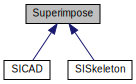
\includegraphics[width=208pt]{classSuperimpose__inherit__graph}
\end{center}
\end{figure}
\subsection*{Public Types}
\begin{DoxyCompactItemize}
\item 
typedef std\+::vector$<$ double $>$ \mbox{\hyperlink{classSuperimpose_a85d40a5caf19f486d1e0c15c0a025378}{Model\+Pose}}
\item 
typedef std\+::multimap$<$ std\+::string, \mbox{\hyperlink{classSuperimpose_a85d40a5caf19f486d1e0c15c0a025378}{Model\+Pose}} $>$ \mbox{\hyperlink{classSuperimpose_a178e3d4e2def6635bfcf9454dd4b5d22}{Model\+Pose\+Container}}
\item 
typedef std\+::pair$<$ std\+::string, \mbox{\hyperlink{classSuperimpose_a85d40a5caf19f486d1e0c15c0a025378}{Model\+Pose}} $>$ \mbox{\hyperlink{classSuperimpose_a1e02e0225687b42296dcfee4eadf8a55}{Model\+Pose\+Container\+Element}}
\end{DoxyCompactItemize}
\subsection*{Public Member Functions}
\begin{DoxyCompactItemize}
\item 
virtual \mbox{\hyperlink{classSuperimpose_a9e32031994dc105b1572e7a6db26b41b}{$\sim$\+Superimpose}} ()
\item 
virtual bool \mbox{\hyperlink{classSuperimpose_a62c4c269b8fc34cc36d3d54fa4acb35c}{superimpose}} (const \mbox{\hyperlink{classSuperimpose_a178e3d4e2def6635bfcf9454dd4b5d22}{Model\+Pose\+Container}} \&objpos\+\_\+map, const double $\ast$cam\+\_\+x, const double $\ast$cam\+\_\+o, cv\+::\+Mat \&img)=0
\end{DoxyCompactItemize}


\subsection{Detailed Description}


Definition at line 20 of file Superimpose.\+h.



\subsection{Member Typedef Documentation}
\mbox{\Hypertarget{classSuperimpose_a85d40a5caf19f486d1e0c15c0a025378}\label{classSuperimpose_a85d40a5caf19f486d1e0c15c0a025378}} 
\index{Superimpose@{Superimpose}!Model\+Pose@{Model\+Pose}}
\index{Model\+Pose@{Model\+Pose}!Superimpose@{Superimpose}}
\subsubsection{\texorpdfstring{Model\+Pose}{ModelPose}}
{\footnotesize\ttfamily typedef std\+::vector$<$double$>$ \mbox{\hyperlink{classSuperimpose_a85d40a5caf19f486d1e0c15c0a025378}{Superimpose\+::\+Model\+Pose}}}



Definition at line 23 of file Superimpose.\+h.

\mbox{\Hypertarget{classSuperimpose_a178e3d4e2def6635bfcf9454dd4b5d22}\label{classSuperimpose_a178e3d4e2def6635bfcf9454dd4b5d22}} 
\index{Superimpose@{Superimpose}!Model\+Pose\+Container@{Model\+Pose\+Container}}
\index{Model\+Pose\+Container@{Model\+Pose\+Container}!Superimpose@{Superimpose}}
\subsubsection{\texorpdfstring{Model\+Pose\+Container}{ModelPoseContainer}}
{\footnotesize\ttfamily typedef std\+::multimap$<$std\+::string, \mbox{\hyperlink{classSuperimpose_a85d40a5caf19f486d1e0c15c0a025378}{Model\+Pose}}$>$ \mbox{\hyperlink{classSuperimpose_a178e3d4e2def6635bfcf9454dd4b5d22}{Superimpose\+::\+Model\+Pose\+Container}}}



Definition at line 25 of file Superimpose.\+h.

\mbox{\Hypertarget{classSuperimpose_a1e02e0225687b42296dcfee4eadf8a55}\label{classSuperimpose_a1e02e0225687b42296dcfee4eadf8a55}} 
\index{Superimpose@{Superimpose}!Model\+Pose\+Container\+Element@{Model\+Pose\+Container\+Element}}
\index{Model\+Pose\+Container\+Element@{Model\+Pose\+Container\+Element}!Superimpose@{Superimpose}}
\subsubsection{\texorpdfstring{Model\+Pose\+Container\+Element}{ModelPoseContainerElement}}
{\footnotesize\ttfamily typedef std\+::pair$<$std\+::string, \mbox{\hyperlink{classSuperimpose_a85d40a5caf19f486d1e0c15c0a025378}{Model\+Pose}}$>$ \mbox{\hyperlink{classSuperimpose_a1e02e0225687b42296dcfee4eadf8a55}{Superimpose\+::\+Model\+Pose\+Container\+Element}}}



Definition at line 27 of file Superimpose.\+h.



\subsection{Constructor \& Destructor Documentation}
\mbox{\Hypertarget{classSuperimpose_a9e32031994dc105b1572e7a6db26b41b}\label{classSuperimpose_a9e32031994dc105b1572e7a6db26b41b}} 
\index{Superimpose@{Superimpose}!````~Superimpose@{$\sim$\+Superimpose}}
\index{````~Superimpose@{$\sim$\+Superimpose}!Superimpose@{Superimpose}}
\subsubsection{\texorpdfstring{$\sim$\+Superimpose()}{~Superimpose()}}
{\footnotesize\ttfamily virtual Superimpose\+::$\sim$\+Superimpose (\begin{DoxyParamCaption}{ }\end{DoxyParamCaption})\hspace{0.3cm}{\ttfamily [inline]}, {\ttfamily [virtual]}}



Definition at line 29 of file Superimpose.\+h.



\subsection{Member Function Documentation}
\mbox{\Hypertarget{classSuperimpose_a62c4c269b8fc34cc36d3d54fa4acb35c}\label{classSuperimpose_a62c4c269b8fc34cc36d3d54fa4acb35c}} 
\index{Superimpose@{Superimpose}!superimpose@{superimpose}}
\index{superimpose@{superimpose}!Superimpose@{Superimpose}}
\subsubsection{\texorpdfstring{superimpose()}{superimpose()}}
{\footnotesize\ttfamily virtual bool Superimpose\+::superimpose (\begin{DoxyParamCaption}\item[{const \mbox{\hyperlink{classSuperimpose_a178e3d4e2def6635bfcf9454dd4b5d22}{Model\+Pose\+Container}} \&}]{objpos\+\_\+map,  }\item[{const double $\ast$}]{cam\+\_\+x,  }\item[{const double $\ast$}]{cam\+\_\+o,  }\item[{cv\+::\+Mat \&}]{img }\end{DoxyParamCaption})\hspace{0.3cm}{\ttfamily [pure virtual]}}



Implemented in \mbox{\hyperlink{classSICAD_a356e0ac8a0f130952a72326bedd4ab60}{S\+I\+C\+AD}}, and \mbox{\hyperlink{classSISkeleton_a3f49fa3419370c2597435768f280c747}{S\+I\+Skeleton}}.



The documentation for this class was generated from the following file\+:\begin{DoxyCompactItemize}
\item 
\mbox{\hyperlink{Superimpose_8h}{Superimpose.\+h}}\end{DoxyCompactItemize}

\hypertarget{structMesh_1_1Texture}{}\section{Mesh\+:\+:Texture Struct Reference}
\label{structMesh_1_1Texture}\index{Mesh\+::\+Texture@{Mesh\+::\+Texture}}


{\ttfamily \#include $<$Mesh.\+h$>$}

\subsection*{Public Attributes}
\begin{DoxyCompactItemize}
\item 
G\+Luint \mbox{\hyperlink{structMesh_1_1Texture_a74c3bcb5a2e98377f722d26a7901e7a5}{id}}
\item 
std\+::string \mbox{\hyperlink{structMesh_1_1Texture_afd1b4cc8fd445ce46e2d5fe5f4238d84}{type}}
\item 
ai\+String \mbox{\hyperlink{structMesh_1_1Texture_aa35695c6acc49df270b0c9d0926654d6}{path}}
\end{DoxyCompactItemize}


\subsection{Detailed Description}


Definition at line 32 of file Mesh.\+h.



\subsection{Member Data Documentation}
\mbox{\Hypertarget{structMesh_1_1Texture_a74c3bcb5a2e98377f722d26a7901e7a5}\label{structMesh_1_1Texture_a74c3bcb5a2e98377f722d26a7901e7a5}} 
\index{Mesh\+::\+Texture@{Mesh\+::\+Texture}!id@{id}}
\index{id@{id}!Mesh\+::\+Texture@{Mesh\+::\+Texture}}
\subsubsection{\texorpdfstring{id}{id}}
{\footnotesize\ttfamily G\+Luint Mesh\+::\+Texture\+::id}



Definition at line 34 of file Mesh.\+h.



Referenced by Model\+::load\+Material\+Textures().

\mbox{\Hypertarget{structMesh_1_1Texture_aa35695c6acc49df270b0c9d0926654d6}\label{structMesh_1_1Texture_aa35695c6acc49df270b0c9d0926654d6}} 
\index{Mesh\+::\+Texture@{Mesh\+::\+Texture}!path@{path}}
\index{path@{path}!Mesh\+::\+Texture@{Mesh\+::\+Texture}}
\subsubsection{\texorpdfstring{path}{path}}
{\footnotesize\ttfamily ai\+String Mesh\+::\+Texture\+::path}



Definition at line 36 of file Mesh.\+h.



Referenced by Model\+::load\+Material\+Textures().

\mbox{\Hypertarget{structMesh_1_1Texture_afd1b4cc8fd445ce46e2d5fe5f4238d84}\label{structMesh_1_1Texture_afd1b4cc8fd445ce46e2d5fe5f4238d84}} 
\index{Mesh\+::\+Texture@{Mesh\+::\+Texture}!type@{type}}
\index{type@{type}!Mesh\+::\+Texture@{Mesh\+::\+Texture}}
\subsubsection{\texorpdfstring{type}{type}}
{\footnotesize\ttfamily std\+::string Mesh\+::\+Texture\+::type}



Definition at line 35 of file Mesh.\+h.



Referenced by Model\+::load\+Material\+Textures().



The documentation for this struct was generated from the following file\+:\begin{DoxyCompactItemize}
\item 
\mbox{\hyperlink{Mesh_8h}{Mesh.\+h}}\end{DoxyCompactItemize}

\hypertarget{structMesh_1_1Vertex}{}\section{Mesh\+:\+:Vertex Struct Reference}
\label{structMesh_1_1Vertex}\index{Mesh\+::\+Vertex@{Mesh\+::\+Vertex}}


{\ttfamily \#include $<$Mesh.\+h$>$}

\subsection*{Public Attributes}
\begin{DoxyCompactItemize}
\item 
glm\+::vec3 \mbox{\hyperlink{structMesh_1_1Vertex_a6c5e0102d84ee335346ef8fadf43ecd0}{Position}}
\item 
glm\+::vec3 \mbox{\hyperlink{structMesh_1_1Vertex_a9e1d54510bff2f84467dfb7b556708a5}{Normal}}
\item 
glm\+::vec2 \mbox{\hyperlink{structMesh_1_1Vertex_a7f4c7ecd20476006a2869452cb2e022b}{Tex\+Coords}}
\end{DoxyCompactItemize}


\subsection{Detailed Description}


Definition at line 25 of file Mesh.\+h.



\subsection{Member Data Documentation}
\mbox{\Hypertarget{structMesh_1_1Vertex_a9e1d54510bff2f84467dfb7b556708a5}\label{structMesh_1_1Vertex_a9e1d54510bff2f84467dfb7b556708a5}} 
\index{Mesh\+::\+Vertex@{Mesh\+::\+Vertex}!Normal@{Normal}}
\index{Normal@{Normal}!Mesh\+::\+Vertex@{Mesh\+::\+Vertex}}
\subsubsection{\texorpdfstring{Normal}{Normal}}
{\footnotesize\ttfamily glm\+::vec3 Mesh\+::\+Vertex\+::\+Normal}



Definition at line 28 of file Mesh.\+h.



Referenced by Model\+::process\+Mesh().

\mbox{\Hypertarget{structMesh_1_1Vertex_a6c5e0102d84ee335346ef8fadf43ecd0}\label{structMesh_1_1Vertex_a6c5e0102d84ee335346ef8fadf43ecd0}} 
\index{Mesh\+::\+Vertex@{Mesh\+::\+Vertex}!Position@{Position}}
\index{Position@{Position}!Mesh\+::\+Vertex@{Mesh\+::\+Vertex}}
\subsubsection{\texorpdfstring{Position}{Position}}
{\footnotesize\ttfamily glm\+::vec3 Mesh\+::\+Vertex\+::\+Position}



Definition at line 27 of file Mesh.\+h.



Referenced by Model\+::process\+Mesh().

\mbox{\Hypertarget{structMesh_1_1Vertex_a7f4c7ecd20476006a2869452cb2e022b}\label{structMesh_1_1Vertex_a7f4c7ecd20476006a2869452cb2e022b}} 
\index{Mesh\+::\+Vertex@{Mesh\+::\+Vertex}!Tex\+Coords@{Tex\+Coords}}
\index{Tex\+Coords@{Tex\+Coords}!Mesh\+::\+Vertex@{Mesh\+::\+Vertex}}
\subsubsection{\texorpdfstring{Tex\+Coords}{TexCoords}}
{\footnotesize\ttfamily glm\+::vec2 Mesh\+::\+Vertex\+::\+Tex\+Coords}



Definition at line 29 of file Mesh.\+h.



Referenced by Model\+::process\+Mesh().



The documentation for this struct was generated from the following file\+:\begin{DoxyCompactItemize}
\item 
\mbox{\hyperlink{Mesh_8h}{Mesh.\+h}}\end{DoxyCompactItemize}

\chapter{File Documentation}
\input{mainpage_8md}
\hypertarget{Mesh_8cpp}{}\section{Mesh.\+cpp File Reference}
\label{Mesh_8cpp}\index{Mesh.\+cpp@{Mesh.\+cpp}}
{\ttfamily \#include \char`\"{}Superimpose\+Mesh/\+Mesh.\+h\char`\"{}}\newline
{\ttfamily \#include $<$string$>$}\newline
{\ttfamily \#include $<$glm/glm.\+hpp$>$}\newline
{\ttfamily \#include $<$glm/gtc/matrix\+\_\+transform.\+hpp$>$}\newline
{\ttfamily \#include $<$glm/gtc/type\+\_\+ptr.\+hpp$>$}\newline
Include dependency graph for Mesh.\+cpp\+:\nopagebreak
\begin{figure}[H]
\begin{center}
\leavevmode
\includegraphics[width=350pt]{Mesh_8cpp__incl}
\end{center}
\end{figure}

\hypertarget{Mesh_8h}{}\section{Mesh.\+h File Reference}
\label{Mesh_8h}\index{Mesh.\+h@{Mesh.\+h}}
{\ttfamily \#include $<$Superimpose\+Mesh/\+Shader.\+h$>$}\newline
{\ttfamily \#include $<$vector$>$}\newline
{\ttfamily \#include $<$assimp/scene.\+h$>$}\newline
{\ttfamily \#include $<$G\+L/glew.\+h$>$}\newline
{\ttfamily \#include $<$glm/vec2.\+hpp$>$}\newline
{\ttfamily \#include $<$glm/vec3.\+hpp$>$}\newline
Include dependency graph for Mesh.\+h\+:\nopagebreak
\begin{figure}[H]
\begin{center}
\leavevmode
\includegraphics[width=350pt]{Mesh_8h__incl}
\end{center}
\end{figure}
This graph shows which files directly or indirectly include this file\+:\nopagebreak
\begin{figure}[H]
\begin{center}
\leavevmode
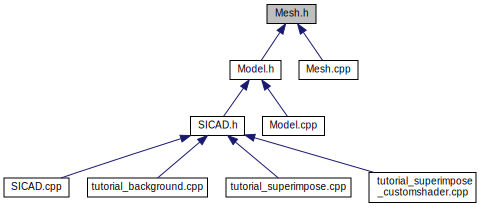
\includegraphics[width=350pt]{Mesh_8h__dep__incl}
\end{center}
\end{figure}
\subsection*{Classes}
\begin{DoxyCompactItemize}
\item 
class \mbox{\hyperlink{classMesh}{Mesh}}
\item 
struct \mbox{\hyperlink{structMesh_1_1Vertex}{Mesh\+::\+Vertex}}
\item 
struct \mbox{\hyperlink{structMesh_1_1Texture}{Mesh\+::\+Texture}}
\end{DoxyCompactItemize}

\hypertarget{Model_8cpp}{}\section{Model.\+cpp File Reference}
\label{Model_8cpp}\index{Model.\+cpp@{Model.\+cpp}}
{\ttfamily \#include \char`\"{}Superimpose\+Mesh/\+Model.\+h\char`\"{}}\newline
{\ttfamily \#include $<$iostream$>$}\newline
{\ttfamily \#include $<$assimp/\+Importer.\+hpp$>$}\newline
{\ttfamily \#include $<$assimp/postprocess.\+h$>$}\newline
{\ttfamily \#include $<$glm/glm.\+hpp$>$}\newline
{\ttfamily \#include $<$opencv2/core/core.\+hpp$>$}\newline
{\ttfamily \#include $<$opencv2/highgui/highgui.\+hpp$>$}\newline
Include dependency graph for Model.\+cpp\+:\nopagebreak
\begin{figure}[H]
\begin{center}
\leavevmode
\includegraphics[width=350pt]{Model_8cpp__incl}
\end{center}
\end{figure}

\hypertarget{Model_8h}{}\section{Model.\+h File Reference}
\label{Model_8h}\index{Model.\+h@{Model.\+h}}
{\ttfamily \#include $<$Superimpose\+Mesh/\+Shader.\+h$>$}\newline
{\ttfamily \#include $<$Superimpose\+Mesh/\+Mesh.\+h$>$}\newline
{\ttfamily \#include $<$vector$>$}\newline
{\ttfamily \#include $<$string$>$}\newline
{\ttfamily \#include $<$assimp/scene.\+h$>$}\newline
{\ttfamily \#include $<$G\+L/glew.\+h$>$}\newline
Include dependency graph for Model.\+h\+:\nopagebreak
\begin{figure}[H]
\begin{center}
\leavevmode
\includegraphics[width=350pt]{Model_8h__incl}
\end{center}
\end{figure}
This graph shows which files directly or indirectly include this file\+:\nopagebreak
\begin{figure}[H]
\begin{center}
\leavevmode
\includegraphics[width=350pt]{Model_8h__dep__incl}
\end{center}
\end{figure}
\subsection*{Classes}
\begin{DoxyCompactItemize}
\item 
class \mbox{\hyperlink{classModel}{Model}}
\end{DoxyCompactItemize}

\hypertarget{Shader_8cpp}{}\section{Shader.\+cpp File Reference}
\label{Shader_8cpp}\index{Shader.\+cpp@{Shader.\+cpp}}
{\ttfamily \#include \char`\"{}Superimpose\+Mesh/\+Shader.\+h\char`\"{}}\newline
{\ttfamily \#include $<$cmrc/cmrc.\+hpp$>$}\newline
{\ttfamily \#include $<$fstream$>$}\newline
{\ttfamily \#include $<$sstream$>$}\newline
{\ttfamily \#include $<$iostream$>$}\newline
Include dependency graph for Shader.\+cpp\+:\nopagebreak
\begin{figure}[H]
\begin{center}
\leavevmode
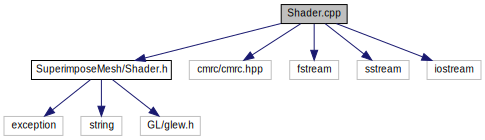
\includegraphics[width=350pt]{Shader_8cpp__incl}
\end{center}
\end{figure}
\subsection*{Functions}
\begin{DoxyCompactItemize}
\item 
\mbox{\hyperlink{Shader_8cpp_a586d93fe18cd555c18d97454a7c95e78}{C\+M\+R\+C\+\_\+\+D\+E\+C\+L\+A\+RE}} (shader)
\end{DoxyCompactItemize}


\subsection{Function Documentation}
\mbox{\Hypertarget{Shader_8cpp_a586d93fe18cd555c18d97454a7c95e78}\label{Shader_8cpp_a586d93fe18cd555c18d97454a7c95e78}} 
\index{Shader.\+cpp@{Shader.\+cpp}!C\+M\+R\+C\+\_\+\+D\+E\+C\+L\+A\+RE@{C\+M\+R\+C\+\_\+\+D\+E\+C\+L\+A\+RE}}
\index{C\+M\+R\+C\+\_\+\+D\+E\+C\+L\+A\+RE@{C\+M\+R\+C\+\_\+\+D\+E\+C\+L\+A\+RE}!Shader.\+cpp@{Shader.\+cpp}}
\subsubsection{\texorpdfstring{C\+M\+R\+C\+\_\+\+D\+E\+C\+L\+A\+R\+E()}{CMRC\_DECLARE()}}
{\footnotesize\ttfamily C\+M\+R\+C\+\_\+\+D\+E\+C\+L\+A\+RE (\begin{DoxyParamCaption}\item[{shader}]{ }\end{DoxyParamCaption})}


\hypertarget{Shader_8h}{}\section{Shader.\+h File Reference}
\label{Shader_8h}\index{Shader.\+h@{Shader.\+h}}
{\ttfamily \#include $<$exception$>$}\newline
{\ttfamily \#include $<$string$>$}\newline
{\ttfamily \#include $<$G\+L/glew.\+h$>$}\newline
Include dependency graph for Shader.\+h\+:\nopagebreak
\begin{figure}[H]
\begin{center}
\leavevmode
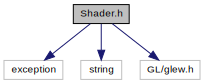
\includegraphics[width=277pt]{Shader_8h__incl}
\end{center}
\end{figure}
This graph shows which files directly or indirectly include this file\+:\nopagebreak
\begin{figure}[H]
\begin{center}
\leavevmode
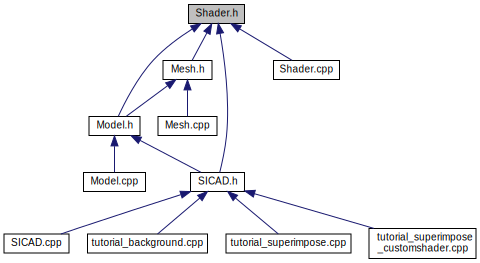
\includegraphics[width=350pt]{Shader_8h__dep__incl}
\end{center}
\end{figure}
\subsection*{Classes}
\begin{DoxyCompactItemize}
\item 
class \mbox{\hyperlink{classShader}{Shader}}
\end{DoxyCompactItemize}

\hypertarget{SICAD_8cpp}{}\section{S\+I\+C\+A\+D.\+cpp File Reference}
\label{SICAD_8cpp}\index{S\+I\+C\+A\+D.\+cpp@{S\+I\+C\+A\+D.\+cpp}}
{\ttfamily \#include \char`\"{}Superimpose\+Mesh/\+S\+I\+C\+A\+D.\+h\char`\"{}}\newline
{\ttfamily \#include $<$iostream$>$}\newline
{\ttfamily \#include $<$exception$>$}\newline
{\ttfamily \#include $<$string$>$}\newline
{\ttfamily \#include $<$assimp/\+Importer.\+hpp$>$}\newline
{\ttfamily \#include $<$assimp/scene.\+h$>$}\newline
{\ttfamily \#include $<$assimp/postprocess.\+h$>$}\newline
{\ttfamily \#include $<$glm/gtc/matrix\+\_\+transform.\+hpp$>$}\newline
{\ttfamily \#include $<$glm/gtc/type\+\_\+ptr.\+hpp$>$}\newline
{\ttfamily \#include $<$opencv2/imgproc/imgproc.\+hpp$>$}\newline
Include dependency graph for S\+I\+C\+A\+D.\+cpp\+:\nopagebreak
\begin{figure}[H]
\begin{center}
\leavevmode
\includegraphics[width=350pt]{SICAD_8cpp__incl}
\end{center}
\end{figure}

\hypertarget{SICAD_8h}{}\section{S\+I\+C\+A\+D.\+h File Reference}
\label{SICAD_8h}\index{S\+I\+C\+A\+D.\+h@{S\+I\+C\+A\+D.\+h}}
{\ttfamily \#include $<$Superimpose\+Mesh/\+Superimpose.\+h$>$}\newline
{\ttfamily \#include \char`\"{}Model.\+h\char`\"{}}\newline
{\ttfamily \#include \char`\"{}Shader.\+h\char`\"{}}\newline
{\ttfamily \#include $<$memory$>$}\newline
{\ttfamily \#include $<$string$>$}\newline
{\ttfamily \#include $<$thread$>$}\newline
{\ttfamily \#include $<$utility$>$}\newline
{\ttfamily \#include $<$vector$>$}\newline
{\ttfamily \#include $<$G\+L/glew.\+h$>$}\newline
{\ttfamily \#include $<$G\+L\+F\+W/glfw3.\+h$>$}\newline
{\ttfamily \#include $<$glm/glm.\+hpp$>$}\newline
Include dependency graph for S\+I\+C\+A\+D.\+h\+:\nopagebreak
\begin{figure}[H]
\begin{center}
\leavevmode
\includegraphics[width=350pt]{SICAD_8h__incl}
\end{center}
\end{figure}
This graph shows which files directly or indirectly include this file\+:\nopagebreak
\begin{figure}[H]
\begin{center}
\leavevmode
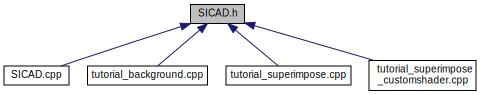
\includegraphics[width=350pt]{SICAD_8h__dep__incl}
\end{center}
\end{figure}
\subsection*{Classes}
\begin{DoxyCompactItemize}
\item 
class \mbox{\hyperlink{classSICAD}{S\+I\+C\+AD}}
\begin{DoxyCompactList}\small\item\em A \mbox{\hyperlink{classSuperimpose}{Superimpose}} derived class to superimpose mesh models on images. \end{DoxyCompactList}\end{DoxyCompactItemize}

\hypertarget{SISkeleton_8cpp}{}\section{S\+I\+Skeleton.\+cpp File Reference}
\label{SISkeleton_8cpp}\index{S\+I\+Skeleton.\+cpp@{S\+I\+Skeleton.\+cpp}}
{\ttfamily \#include \char`\"{}Superimpose\+Mesh/\+S\+I\+Skeleton.\+h\char`\"{}}\newline
{\ttfamily \#include $<$iostream$>$}\newline
{\ttfamily \#include $<$glm/gtc/matrix\+\_\+transform.\+hpp$>$}\newline
{\ttfamily \#include $<$glm/gtc/type\+\_\+ptr.\+hpp$>$}\newline
{\ttfamily \#include $<$opencv2/core/core.\+hpp$>$}\newline
{\ttfamily \#include $<$opencv2/calib3d/calib3d.\+hpp$>$}\newline
{\ttfamily \#include $<$opencv2/imgproc/imgproc.\+hpp$>$}\newline
Include dependency graph for S\+I\+Skeleton.\+cpp\+:\nopagebreak
\begin{figure}[H]
\begin{center}
\leavevmode
\includegraphics[width=350pt]{SISkeleton_8cpp__incl}
\end{center}
\end{figure}

\hypertarget{SISkeleton_8h}{}\section{S\+I\+Skeleton.\+h File Reference}
\label{SISkeleton_8h}\index{S\+I\+Skeleton.\+h@{S\+I\+Skeleton.\+h}}
{\ttfamily \#include \char`\"{}Superimpose.\+h\char`\"{}}\newline
{\ttfamily \#include $<$list$>$}\newline
{\ttfamily \#include $<$string$>$}\newline
{\ttfamily \#include $<$glm/glm.\+hpp$>$}\newline
Include dependency graph for S\+I\+Skeleton.\+h\+:\nopagebreak
\begin{figure}[H]
\begin{center}
\leavevmode
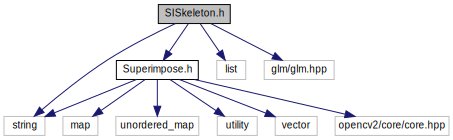
\includegraphics[width=350pt]{SISkeleton_8h__incl}
\end{center}
\end{figure}
This graph shows which files directly or indirectly include this file\+:\nopagebreak
\begin{figure}[H]
\begin{center}
\leavevmode
\includegraphics[width=163pt]{SISkeleton_8h__dep__incl}
\end{center}
\end{figure}
\subsection*{Classes}
\begin{DoxyCompactItemize}
\item 
class \mbox{\hyperlink{classSISkeleton}{S\+I\+Skeleton}}
\end{DoxyCompactItemize}

\hypertarget{Superimpose_8h}{}\section{Superimpose.\+h File Reference}
\label{Superimpose_8h}\index{Superimpose.\+h@{Superimpose.\+h}}
{\ttfamily \#include $<$string$>$}\newline
{\ttfamily \#include $<$map$>$}\newline
{\ttfamily \#include $<$unordered\+\_\+map$>$}\newline
{\ttfamily \#include $<$utility$>$}\newline
{\ttfamily \#include $<$vector$>$}\newline
{\ttfamily \#include $<$opencv2/core/core.\+hpp$>$}\newline
Include dependency graph for Superimpose.\+h\+:\nopagebreak
\begin{figure}[H]
\begin{center}
\leavevmode
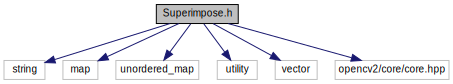
\includegraphics[width=350pt]{Superimpose_8h__incl}
\end{center}
\end{figure}
This graph shows which files directly or indirectly include this file\+:\nopagebreak
\begin{figure}[H]
\begin{center}
\leavevmode
\includegraphics[width=350pt]{Superimpose_8h__dep__incl}
\end{center}
\end{figure}
\subsection*{Classes}
\begin{DoxyCompactItemize}
\item 
class \mbox{\hyperlink{classSuperimpose}{Superimpose}}
\end{DoxyCompactItemize}

\hypertarget{tutorial__background_8cpp}{}\section{tutorial\+\_\+background.\+cpp File Reference}
\label{tutorial__background_8cpp}\index{tutorial\+\_\+background.\+cpp@{tutorial\+\_\+background.\+cpp}}
{\ttfamily \#include $<$cmath$>$}\newline
{\ttfamily \#include $<$exception$>$}\newline
{\ttfamily \#include $<$iostream$>$}\newline
{\ttfamily \#include $<$string$>$}\newline
{\ttfamily \#include $<$glm/glm.\+hpp$>$}\newline
{\ttfamily \#include $<$glm/gtc/matrix\+\_\+transform.\+hpp$>$}\newline
{\ttfamily \#include $<$opencv2/core/core.\+hpp$>$}\newline
{\ttfamily \#include $<$opencv2/imgcodecs/imgcodecs.\+hpp$>$}\newline
{\ttfamily \#include $<$opencv2/imgproc/imgproc.\+hpp$>$}\newline
{\ttfamily \#include $<$Superimpose\+Mesh/\+S\+I\+C\+A\+D.\+h$>$}\newline
Include dependency graph for tutorial\+\_\+background.\+cpp\+:\nopagebreak
\begin{figure}[H]
\begin{center}
\leavevmode
\includegraphics[width=350pt]{tutorial__background_8cpp__incl}
\end{center}
\end{figure}
\subsection*{Functions}
\begin{DoxyCompactItemize}
\item 
int \mbox{\hyperlink{tutorial__background_8cpp_ae66f6b31b5ad750f1fe042a706a4e3d4}{main}} ()
\end{DoxyCompactItemize}


\subsection{Function Documentation}
\mbox{\Hypertarget{tutorial__background_8cpp_ae66f6b31b5ad750f1fe042a706a4e3d4}\label{tutorial__background_8cpp_ae66f6b31b5ad750f1fe042a706a4e3d4}} 
\index{tutorial\+\_\+background.\+cpp@{tutorial\+\_\+background.\+cpp}!main@{main}}
\index{main@{main}!tutorial\+\_\+background.\+cpp@{tutorial\+\_\+background.\+cpp}}
\subsubsection{\texorpdfstring{main()}{main()}}
{\footnotesize\ttfamily int main (\begin{DoxyParamCaption}{ }\end{DoxyParamCaption})}



Definition at line 14 of file tutorial\+\_\+background.\+cpp.



References S\+I\+C\+A\+D\+::set\+Background\+Opt(), and S\+I\+C\+A\+D\+::superimpose().

Here is the call graph for this function\+:\nopagebreak
\begin{figure}[H]
\begin{center}
\leavevmode
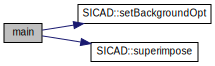
\includegraphics[width=287pt]{tutorial__background_8cpp_ae66f6b31b5ad750f1fe042a706a4e3d4_cgraph}
\end{center}
\end{figure}

\input{tutorial__superimpose_8cpp}
\hypertarget{tutorial__superimpose_8md}{}\section{tutorial\+\_\+superimpose.\+md File Reference}
\label{tutorial__superimpose_8md}\index{tutorial\+\_\+superimpose.\+md@{tutorial\+\_\+superimpose.\+md}}

\hypertarget{tutorial__superimpose__background_8md}{}\section{tutorial\+\_\+superimpose\+\_\+background.\+md File Reference}
\label{tutorial__superimpose__background_8md}\index{tutorial\+\_\+superimpose\+\_\+background.\+md@{tutorial\+\_\+superimpose\+\_\+background.\+md}}

\hypertarget{tutorial__superimpose__customshader_8cpp}{}\section{tutorial\+\_\+superimpose\+\_\+customshader.\+cpp File Reference}
\label{tutorial__superimpose__customshader_8cpp}\index{tutorial\+\_\+superimpose\+\_\+customshader.\+cpp@{tutorial\+\_\+superimpose\+\_\+customshader.\+cpp}}
{\ttfamily \#include $<$Superimpose\+Mesh/\+S\+I\+C\+A\+D.\+h$>$}\newline
{\ttfamily \#include $<$cmath$>$}\newline
{\ttfamily \#include $<$exception$>$}\newline
{\ttfamily \#include $<$iostream$>$}\newline
{\ttfamily \#include $<$glm/gtc/matrix\+\_\+transform.\+hpp$>$}\newline
{\ttfamily \#include $<$opencv2/core/core.\+hpp$>$}\newline
{\ttfamily \#include $<$opencv2/imgcodecs/imgcodecs.\+hpp$>$}\newline
{\ttfamily \#include $<$opencv2/imgproc/imgproc.\+hpp$>$}\newline
Include dependency graph for tutorial\+\_\+superimpose\+\_\+customshader.\+cpp\+:\nopagebreak
\begin{figure}[H]
\begin{center}
\leavevmode
\includegraphics[width=350pt]{tutorial__superimpose__customshader_8cpp__incl}
\end{center}
\end{figure}
\subsection*{Functions}
\begin{DoxyCompactItemize}
\item 
int \mbox{\hyperlink{tutorial__superimpose__customshader_8cpp_ae66f6b31b5ad750f1fe042a706a4e3d4}{main}} ()
\end{DoxyCompactItemize}


\subsection{Function Documentation}
\mbox{\Hypertarget{tutorial__superimpose__customshader_8cpp_ae66f6b31b5ad750f1fe042a706a4e3d4}\label{tutorial__superimpose__customshader_8cpp_ae66f6b31b5ad750f1fe042a706a4e3d4}} 
\index{tutorial\+\_\+superimpose\+\_\+customshader.\+cpp@{tutorial\+\_\+superimpose\+\_\+customshader.\+cpp}!main@{main}}
\index{main@{main}!tutorial\+\_\+superimpose\+\_\+customshader.\+cpp@{tutorial\+\_\+superimpose\+\_\+customshader.\+cpp}}
\subsubsection{\texorpdfstring{main()}{main()}}
{\footnotesize\ttfamily int main (\begin{DoxyParamCaption}{ }\end{DoxyParamCaption})}



Definition at line 14 of file tutorial\+\_\+superimpose\+\_\+customshader.\+cpp.



References S\+I\+C\+A\+D\+::superimpose().

Here is the call graph for this function\+:\nopagebreak
\begin{figure}[H]
\begin{center}
\leavevmode
\includegraphics[width=261pt]{tutorial__superimpose__customshader_8cpp_ae66f6b31b5ad750f1fe042a706a4e3d4_cgraph}
\end{center}
\end{figure}

%--- End generated contents ---

% Index
\backmatter
\newpage
\phantomsection
\clearemptydoublepage
\addcontentsline{toc}{chapter}{Index}
\printindex

\end{document}
